% IFO configs (jupyter notebooks)

% Paraxial equation

% Cavity Stability criteria

% The Equipartition theorem and the Fluctuation Dissapation theorem

% Monochromatic plane wave propogation

% The Dielectric Tensor

% Thermo-optic Path Distortion (analytical)
% Transient thermo-optic responses
    %% Thermal Lens Optical Path Distortion (Hello-Vinet)
    %% COMSOL self heating filter
    %% RH actuation
	%%% Analytical solution
	%%% Conditioned RH input filter
    %% CO2 filters

% CO2 mask

% Miller indices for highly reflective \texorpdfstring{$\gaas$ / $\algaas$} coatings

% Mode matching data for Electro-optic sample cavity
    %% Pre MMT beam scan
    %% ``Just another mode matching tool" (JAMMT) solution
    %% Post MMT beam scan

% Laser PZT sweep

% Assembly blueprints and alternative views
    %% Assembly 1
	%%% Cross section
    	%%% Electrodes
    	%%% Iteration 1.1
    	%%% Iteration 1.2
    	%%% Iteration 1.3
    %% Assembly 2
	%%% Cross section
    	%%% Electrodes
    	%%% Iteration 2.1
    	%%% Iteration 2.2
    	%%% 3D printed with MACOR spacers
    %% Assembly 3
	%%% Cross section
    	%%% Electrodes
    	%%% Iteration 3.0

% LaplacE code
    %% laplacedotpy
    %% set\_paramsdotpy
    %% rundotipynb
% Calibration code

% HVA

% FSS

% Measuring OLG

\section{Interferometer Configurations (code)}\label{appendix:ifo_configs_code}
\subsection{ifo\_configs.py}
\begin{spacing}{1}
\begin{lstlisting}[frame=single, language=Python]
import numpy as np

# Bode tools 
def bode_amp(H):
    """
    Returns amplitude information on transfer function (H)
    """
    return np.sqrt(np.real(H)**2 + np.imag(H)**2)

def bode_ph(H):
    """
    Returns phase information on transfer function (H)
    """
    return (180/np.pi)*np.arctan(np.imag(H)/np.real(H))

# some constants:
cee = np.float64(299792458) ## speed of light [m/s]
h_bar = (6.626e-34)/(2*np.pi) ## planck's constant


# IFO params
def finesse(r_i, r_e):
    """
    r_i : ITM reflectivity coefficient
    r_e : ETM reflectivity coefficient
    """
    return np.pi*np.sqrt(r_i*r_e)/(1-(r_i*r_e))


# Michelson frequency response
def mich_freq_resp(freq, Length, phi_0, P_in, OMEGA):
    """ 
    MICHELSON FREQEUNCY RESPONSE CALCULATOR
    freq : standard (gravitational wave) frequency [Hz]
    Length : Michelson ifo arm length [m]
    phi_0 : static differential arm length tuning phase [rad]
    P_in : input power [W] 
    """
    return (P_in*OMEGA*np.sin(phi_0))*Length*
	    np.exp((-1j*Length*2.0*np.pi*freq)/cee)*
	    np.sin((Length*2.0*np.pi*freq)/cee)/(Length*2.0*np.pi*freq)

def fpmi_freq_resp(freq, r_1, t_1, r_2, L, phi_0, P_in, OMEGA, low_pass=False):
    """
    FABRY PEROT MICHELSON FREQUENCY RESPONSE CALCULATOR
    freq : standard (gravitational wave) frequency [Hz]
    r_1, t_1, r_2: Assuming arm symmetry where the ITM has r_1, t_1 coefficients 
		   and the ETM has a r_2 reflectivity coefficient. 
		   Also assumes no loss. [arb]
    OMEGA: OPTICAL angular frequency [rad Hz]
    Length: Michelson ifo arm length [m]
    phi_0 : static differential arm length tuning phase [rad]
    """
    if low_pass:
        f_pole = 1/(((4*np.pi*L)*np.sqrt(r_1*r_2))/(cee*(1-r_1*r_2)))
        fpmi_resp = 1/(1 + 1j*(freq/f_pole))
    else:
        fpmi_resp = ((t_1**2 * r_2)/((t_1**2 + r_1**2)*r_2 - r_1))*
		    (mich_freq_resp(freq, L, phi_0, P_in, OMEGA)/
		    (1-r_1*r_2*np.exp(-1j*L*4.0*np.pi*freq/cee)))
    return fpmi_resp

def PRG(L_rt, Finn, r_PRM, max=0):
    """
    POWER RECYCLING GAIN (@ optimal reflectivity)
    * Assuming a FPMI with symmetric arms *
    L_rt : Round trip loss
    Finn : Cavity finesse
    """
    if max == 1:
        G_PR = np.pi/(2*Finn*L_rt*(1-((Finn*L_rt)/(2*np.pi))))
    else:
        G_PR = (1-r_PRM**2)/(1-r_PRM*(1-(Finn/np.pi)*L_rt))**2


    return G_PR

def drfpmi_freq_resp(freq, G_PRC_opt, r_1, t_1, r_2, r_SRM, t_SRM, phi_SRC, L, 
		     phi_0, P_in, OMEGA):
    """
    DUAL RECYCLED FABRY PEROT MICHELSON FREQUENCY RESPONSE 
    CALCULATOR

    freq: standard (gravitational wave) frequency [Hz]
    G_PRC_opt: maximum power recycling gain (optimal) [arb]
    r_1: ITM reflection coefficient [arb]
    t_1: ITM transmission coefficient [arb]
    r_2: ETM reflection coefficient [arb]
    r_SRM: Signal recycling mirror reflection coefficient [arb]
    t_SRM: Signal recycling mirror transmission coefficient [arb]
    L: Length of the Fabry-Perot arms [m]
    OMEGA: OPTICAL angular frequency [rad Hz]
    """
    r_SRC = (r_1 - r_SRM*np.exp(1j*2*phi_SRC))/
	    (1 - r_1*r_SRM*np.exp(1j*2*phi_SRC))
    t_SRC = t_1*t_SRM*np.exp(1j*phi_SRC)/(1 - r_1*r_SRM*np.exp(1j*2*phi_SRC))

    return ((t_1**2 * r_2)/((t_1**2 + r_1**2)*r_2 - r_1))*
	    G_PRC_opt*t_SRC*(P_in*L*OMEGA*np.exp((-1j*L*2.0*np.pi*freq)/cee)*
	    np.sin((L*2.0*np.pi*freq)/cee)/(L*2.0*np.pi*freq))/
	    (1-r_SRC*r_2*np.exp(-1j*L*4.0*np.pi*freq/cee))


# Shot noise
def N_shot(OMEGA, P_in):
    """
    Interferometer shot noise calculator
    OMEG: OPTICAL angular frequency [rad Hz]
    Length : ifo arm length [m]
    phi_0 : static differential arm length tuning phase [rad]
    P_in : Input power [W]
    """
    return np.sqrt(2*h_bar*OMEGA*P_in)
\end{lstlisting}
\end{spacing}


\subsection{MICH}\label{appendix:MICH}
\begin{spacing}{1.2} \begin{lstlisting}[frame=single, language=Python]
import numpy as np
import matplotlib.pyplot as plt
import os
import sys
sys.path.insert(0,'../')
plt_style_dir = '../../stash/'
fig_exp_dir = '../../../figs/'
from ifo_configs import N_shot
from ifo_configs import mich_freq_resp as MICH
from ifo_configs import bode_amp, bode_ph
%matplotlib inline
if os.path.isdir(plt_style_dir) == True:
    plt.style.use(plt_style_dir + 'ppt2latexsubfig.mplstyle')
plt.rcParams["font.family"] = "Times New Roman"
\end{lstlisting} \end{spacing}

\begin{spacing}{1.2} \begin{lstlisting}[frame=single, language=Python]
# Some parameters
cee = np.float64(299792458)
h_bar = (6.626e-34)/(2*np.pi)
OMEG = np.float64(2*np.pi*cee/(1064.0*1e-9))
L = np.float64(4000.0)
nu = np.arange(1, 1000000, 1)
PHI_0 = np.pi/2 #[rad]
P_IN = 125 #[W]
\end{lstlisting} \end{spacing}

\hypertarget{derivation}{%
\subsubsection{Derivation}\label{derivation}}

For the simple Michelson we know that a change in arm length correlates
to light at the AS port We also know that a differential arm length
corresponds to a difference in phase of the light that impinges upon the
BS For a gravitational wave we can quantify the phase difference in this
following way:

\begin{equation}
\phi_A - \phi_B = \int_{t-2L/c}^{t} \Omega \bigg[1 + \frac{1}{2}h(t)\bigg]dt - \int_{t-2L/c}^{t} \Omega \bigg[1 - \frac{1}{2}h(t)\bigg]dt 
\end{equation} The phase difference can then be quantified by: \begin{equation}
\phi_A - \phi_B = \int_{t-2L/c}^{t} \Omega h(t)dt 
\end{equation} where \begin{equation} 
h(t) = h_0 e^{i \omega t} 
\end{equation}

\noindent \emph{\(\Omega\)} is the \textbf{optical angular frequency}

\noindent After evaluating this integral we get: 
\begin{equation}
\Delta \phi=\phi_A - \phi_B = \frac{2 L \Omega}{c}e^{-i L \omega / c} \frac{\mathrm{sin}(L \omega /c)}{L \omega /c} \cdot h_0 e^{i \omega t}
\end{equation}

\noindent Where the first term in the phase difference carries all the time
independent frequency information. This is what we are calculating
below.

\noindent For the sake of being explicit, we are going to plot: 
\begin{equation}
\Delta \phi (\omega) = h_0\frac{2 L \Omega}{c}e^{-i L \omega / c} \frac{\mathrm{sin}(L \omega /c)}{L \omega /c}
\end{equation}This accounts for the differential phase as a function of
gravitational wave frequency, though we have not established the amount
of optical gain the Michelson offers. This can be understood through a
first order taylor approximation about a selected Michelson offset angle
\(\phi_0\):

\begin{equation}P(\omega, \phi_0) =  \frac{P_\mathrm{in}}{4} [r_x^2 + r_y^2 -  2r_x r_y\mathrm{cos}(\phi_0 + \Delta \phi (\omega)] \end{equation}

\begin{equation}P(\omega, \phi_0) \approx  \frac{P_\mathrm{in}}{4} \Big[ r_x^2 + r_y^2 -  2r_x r_y \big(\mathrm{cos}(\phi_0) - \Delta \phi(\omega) \cdot \mathrm{sin}(\phi_0) \big) \Big] =  \frac{P_\mathrm{in}}{2} \Big[1 - \big(\mathrm{cos}(\phi_0) - \Delta \phi(\omega) \cdot \mathrm{sin}(\phi_0) \big) \Big]\end{equation}

\noindent Where we define a response gain function \(H_\mathrm{MICH}\):

\begin{equation}\mathrm{H}_\mathrm{MICH}(\omega, \phi_0) =   \frac{P_\mathrm{in}}{2} \cdot \Delta \phi(\omega) \cdot \mathrm{sin}(\phi_0)\end{equation}

\begin{spacing}{1.2} \begin{lstlisting}[frame=single, language=Python]
H = MICH(nu, L, PHI_0, P_IN, OMEG)
\end{lstlisting} \end{spacing}

\begin{spacing}{1.2} \begin{lstlisting}[frame=single, language=Python]
fig, ax1 = plt.subplots()
ax1.set_xlabel('frequency [Hz]')
ax1.set_ylabel('H$_{\mathdefault{MICH}}$ [$\mathdefault{W/m}$]',color='C0')
#ax1.plot(w/(FSR), F_w_cc_modsq*100)
ax1.loglog(bode_amp(H),linewidth=7.5, color='C0')
#plt.ylim([10e-6, 10e0])
ax2 = ax1.twinx()
#ax2.plot(w/(FSR), (180/np.pi)*np.arctan(F_w_cc.imag/F_w_cc.real), '--')
ax2.semilogx(nu,(180/np.pi)*np.arctan(np.imag(H)/np.real(H)), '--', linewidth=7.5,
	     color='C1')
#plt.xlabel('frequency [FSR]')
plt.xlim([1,1e5])
plt.ylabel('phase [deg]',color='C1')
fig.savefig(fig_exp_dir + 'INTRO/mich_fr.pdf', dpi=300, bbox_inches='tight')
\end{lstlisting} \end{spacing}

Though with the provided frequency depdenence and optical gain, we still
need to understand a starting noise floor spectra and compare to our
anticipated limiting noise 

\noindent\textbf{Shot noise} 
\\
* A fundamental limit imposed by the statistical nature of photon counting 
\\
* The photon counting follows Poisson statistics 
\\
\indent    * Photon counting variance (variance is equal to the
mean) 
\begin{equation} < (n-\bar{n})^2 >  = \frac{P \Delta t}{ \hbar \Omega} \end{equation} 
\indent * Power variance:
\begin{equation} < (P - \bar{P})^2 >  = \hbar \Omega  \bar{P} \Delta t \end{equation} 
\indent * PSD of the measured power between two uncoorelated moments in time:
\begin{equation} S_\mathrm{P} (\omega) = \lim_{T \to \infty} \frac{2}{T} \Big< \big| \int_{-T}^{T} (P(t) - \bar{P}) e^{-i\omega t} dt \big|^2 \Big> \end{equation}
\begin{equation} =  \lim_{T \to \infty} \frac{2}{T} \int_{-T}^{T} \hbar \Omega \bar{P} dt  \end{equation}
\begin{equation} = 2 \hbar \Omega \bar{P} \end{equation} 
\indent * Where the ASD is:
\begin{equation} [S_P (\omega)]^{1/2} = [2 \hbar \Omega \bar{P}]^{1/2}\end{equation}The signal to
noise is established by dividing the frequency dependent optical gain
times the gravitational wave ASD
\(\big( [\mathrm{S}_{\mathrm{h}}(\Omega)]^{1/2} \big)\) by the noise
ASD:

\begin{equation}\mathrm{SNR} = \mathrm{G_{opt}(\omega)} [\mathrm{S}_{\mathrm{h}}(\omega)]^{1/2} / S_\mathrm{N}(\omega) = \mathrm{H}_\mathrm{MICH} / [S_P]^{1/2} = \bigg( \frac{\Delta \phi(\omega)}{h_0} \frac{P_\mathrm{in}}{2}\mathrm{sin}(\phi_0) \bigg) \bigg/ [2 \hbar \Omega \bar{P}]^{1/2}\end{equation}

\noindent This is to say that for the stated gravitational wave ASD, and for an
SNR of 1, we establish the following threshold for detector:

\begin{equation}\big[ \mathrm{S}_{\mathrm{h}}(\omega) \big]^{1/2} \; \{\mathrm{SNR}\geq1\} \geq \frac{ [S_\mathrm{N}(\omega)]^{1/2}}{\mathrm{H}_\mathrm{MICH}(\omega)}\end{equation}

\noindent Where

\begin{equation}\frac{ [S_\mathrm{N}(\omega)]^{1/2}}{\mathrm{H}_\mathrm{MICH}(\omega)} = \frac{[2 \hbar \omega \bar{P}]^{1/2}}{ \Delta \phi(\omega) [P_\mathrm{in} / 2]  \mathrm{sin}(\phi_0)} = \bigg( \frac{\hbar \Omega }{\omega P_\mathrm{in}} \bigg)^{1/2} \frac{[r_x^2 + r_y^2 -  2r_x r_y\mathrm{cos}(\phi_0)]^{1/2}}{\mathrm{sin}(L \omega / c)} e^{iL \omega / c}\end{equation}

\begin{spacing}{1.2} \begin{lstlisting}[frame=single, language=Python]
S_h = N_shot(OMEG, P_IN) 
print(S_h)
\end{lstlisting} \end{spacing}

\begin{spacing}{1.2} \begin{lstlisting}[frame=single, language=Python]
#ax1.plot(w/(FSR), F_w_cc_modsq*100)
plt.loglog(nu, S_h/bode_amp(H), linewidth=7.5, color='C0')
plt.ylim([1e-21, .5e-14])
plt.xlabel('frequency [Hz]')
plt.ylabel('$\mathdefault{S}_\mathdefault{h} \;  
	    \mathdefault{[ 1 / \sqrt{\mathdefault{Hz}}]} $')
#ax2_ = ax1_.twinx()
#ax2.plot(w/(FSR), (180/np.pi)*np.arctan(F_w_cc.imag/F_w_cc.real), '--')
#ax2_.semilogx(nu,(180/np.pi)*np.arctan(np.imag(S_h)/np.real(S_h)), '--', 
	       linewidth=7.5,color='C1')
#plt.xlabel('frequency [FSR]')
plt.xlim([1,1e5])
plt.grid(visible=True)
#plt.subplots_adjust(hspace = 1)
#plt.ylabel('phase [deg]',color='C1')
#plt.tight_layout(rect=[0,0,1,1])
#plt.title('')
#plt.subplots_adjust(bottom=.1, top=.85) #, right=.8, left=.1)
plt.savefig(fig_exp_dir + 'INTRO/mich_sensi.pdf', dpi=300, bbox_inches='tight')
\end{lstlisting} \end{spacing}



\subsection{FPMI}\label{appendix:FPMI}
\begin{lstlisting}[frame=single, language=Python]
import numpy as np 
import matplotlib.pyplot as plt
import scipy.signal as sig
import os
import sys
sys.path.insert(0,'../')
plt_style_dir = '../../stash/'
fig_exp_dir = '../../../figs/'
from ifo_configs import mich_freq_resp as MICH
from ifo_configs import fpmi_freq_resp as FPMI
from ifo_configs import N_shot, bode_amp, bode_ph
if os.path.isdir(plt_style_dir) == True:
    plt.style.use(plt_style_dir + 'ppt2latexsubfig.mplstyle')
plt.rcParams["font.family"] = "Times New Roman"
line_width=7.5
\end{lstlisting}

Let's start with the simple Fabry Perót cavity. The following are
equations that characterize the circulating and reflected fields (both
critical to measuring the phase response of the FP cavity to GWs):

\[
E(t) = t_1 E_{in} + r_1 r_2 E(t - 2T) e^{-i \Delta \phi(t)} 
\]

\[
E_r(t) = -r_1 E_{in} + t_1 r_2 E(t - 2T) e^{-i \Delta \phi(t)}
\]

\(T = L/c\) is the time it takes light to reach the end of the cavity
and \(\Delta \phi(t)\) is the phase rotation.

We can define the static phase rotation (no GW passing through) as :
\[\Delta \phi = 2kL = 4 \pi L /\lambda_{opt}  \]

And if L is tuned just right \(2kL = 2 \pi n\) so the cavity is just
tuned for resonance

If we put a gravitational wave in the mix we redefine this phase
rotation as such that:
\[\Delta \phi =  \frac{\omega_0}{2} \int_{t-\frac{2L}{c}}^{t} h(t')dt' \]

This assumes that the static phase rotation satisfies
\(2\omega_0L/c = 2 \pi n\). Which is the same thing that we said above
but with different symbols (because we're fancy ;D )

Say that we have something that does throw the cavity slightly off
resonance.. doesn't have to be a gravitational wave\ldots{} but that's
what we hope for. ANYWAY\ldots{}

If the \(\Delta \phi\) becomes such that the cavity is thrown off
resonance we get a time dependent intra-cavity field:

\[ E(t) = \bar{E} + \delta E(t) \]

and if the phase rotation (\(\Delta \phi\)) is super small\ldots{} which
is pretty much guaranteed with gravy waves, we can say:

\[ e^{i\Delta \phi} = 1- i \Delta \phi \]

Using equations \ref{eq7} and \ref{eq8} in \ref{eq3} we get:

\[ \bar{E} + \delta E(t) = t_1 E_{in} -r_1r_2\bar{E} + r_1r_2 \delta E(t-2T) - ir_1r_2\bar{E}\Delta \phi(t)) \]

We can parse this into time dependent and time independent terms:

\[ \bar{E} = t_1 E_{in} -r_1r_2\bar{E} \]

\[ \delta E(t) = r_1r_2 \delta E(t-2T) - ir_1r_2\bar{E}\Delta \phi(t) \]

Since the time dependent phase information is encoded in \ref{eq11} we
will take the laplace transform of this equation to yield:

\[\delta E(s) = -i \frac{r_1r_2 \bar{E}}{1-r_1r_2e^{-2sT}} \Delta \phi(s)\]

\textbf{YAS!} we are now one step closer to getting a useful expression
for the phase response. But again.. what does this last equation mean?
That last equation is how the change in the electric field directly
relates to a small perturbation in phase (which could be either a small
change in laser frequency or length modulation)

Now.. we're not done yet because that last expression does not tell us
the entire story yet.. we want to see how this effects the phase
differential with the \textbf{reflected} electric field.

To do this.. we have to combine equations \ref{eq3} and \ref{eq4}. (an
easy way to do this is to get rid of the $ r_2 E(t - 2T) e^{-i \Delta \phi(t)} $ ) :

\[ E_r(t) = \frac{t_1}{r_1}E(t) - \frac{t_1^2 + r_2^2}{r_1} E_{in}\]

if the cavity is unperturbed:

\[ \bar{E}_r = \bigg(\frac{r_2(r_1^2 + t_1^2) - r_1}{t_1} \bigg) \bar{E} \]

and if we perturb the cavity we see that the change in the intra-cavity
field is directly related to the change in the reflected field:

\[ \Delta \phi_r(s) \equiv \frac{\delta E(s)}{\bar{E}} = \frac{t_1^2r_2}{(t_1^2 + r_1^2)r_2 -r_1} \frac{\Delta \phi(s)}{1-r_1r_2e^{-2sT}}\]

This implies that there is an additional frequency dependent factor in
your phase shift and this translates into your FPMI transfer function
as:

\[ H_{FPMI}(\omega_g) = \frac{2 \Delta \phi_r(\omega_g)}{h(\omega_g)} =  \frac{t_1^2r_2}{(t_1^2 + r_1^2)r_2 -r_1} \frac{H_{\mathrm{MI}}(\omega_g, L)}{1-r_1r_2e^{-2i \omega_g L /c }}  \]

Whew\ldots. that was a lot\ldots. now let's code it up Since we can
seperate the calculation into two.. I'm going to parse out the
calculation between the constant Fabry Perót term and the term with the
frequency dependence. But first, lets set up our parameters for our
FPMI:

\begin{lstlisting}[frame=single, language=Python]
# Some parameters
cee = np.float64(299792458)
OMEG = np.float64(2*np.pi*cee/(1064.0*1e-9))
L = np.float64(4000.0)
nu = np.arange(1, 1000000, 1)
nat_nu = [np.float64(i*2*np.pi) for i in nu]
h_0 = np.float64(1)

PHI_0 = np.pi/2 #[rad]
P_IN = 25

T_1 = .014
#T_1 = 25e-6 
T_2 = 50e-6
R_1 = 1-T_1
R_2 = 1-T_2

t_1 = T_1**.5
r_1 = R_1**.5
r_2 = R_2**.5
\end{lstlisting}

Now we can compute:
\[ H_{FPMI}(\omega_g) =  \frac{t_1^2r_2}{(t_1^2 + r_1^2)r_2 -r_1}\cdot \frac{H_{\mathrm{MI}}(\omega_g, L)}{1-r_1r_2e^{-2i \omega_g L /c }}  \]

\begin{lstlisting}[frame=single, language=Python]
H_FPMI = FPMI(nu, r_1, t_1, r_2, L, PHI_0, P_IN, OMEG)
\end{lstlisting}

We estimate the FP's pole frequency
\[  1 - r_1 r_2 e^{-2i \omega_g L / c} = 0 \] therefore when:
\[ e^{-i \omega_g L / c} = \frac{1}{\sqrt{r_1 r_2}} \] we acquire the
pole frequency \(\omega_\mathrm{pole}\) as indicated in the low pass
\[ f_\mathrm{pole} = \frac{1}{4\pi \tau_{s}} =  \frac{c}{4 \pi L} \frac{1- r_1 r_2}{\sqrt{r_1 r_2}} = \frac{\nu_\mathrm{FSR}}{2 \pi} \frac{1- r_1 r_2}{\sqrt{r_1 r_2}} = \frac{\nu_\mathrm{FSR}}{\mathcal{F}} \]

ALso, understanding that the cavity Finesse can be defined as

\[ \mathcal{F} = \frac{\pi \sqrt{r_i r_e}}{1- r_i r_e} \]

we also can invert for a high value of finesse $ \mathcal{F} \textgreater\textgreater{} \pi $:

\[ r_i r_e \approx 1 - \frac{\pi}{\mathcal{F}} \]

\begin{lstlisting}[frame=single, language=Python]
f_pole = 1/(((4*np.pi*L)*np.sqrt(r_1*r_2))/(cee*(1-r_1*r_2)))
def fpmi_lp(freq, cav_pole):
    return 1/(1 + 1j*(freq/cav_pole))#*np.exp(1j*freq/cav_pole))
H_FPMI_LP = fpmi_lp(nu, f_pole)
\end{lstlisting}

Might as well compare it to our Michelson response:
\[ H_{\mathrm{MI}}(\omega_g) = \frac{2 L \Omega}{c}e^{-i L \omega / c} \frac{\mathrm{sin}(L \omega /c)}{L \omega /c} \]

\begin{lstlisting}[frame=single, language=Python]
H_MICH = MICH(nu, L, PHI_0, P_IN, OMEG)
\end{lstlisting}

\begin{lstlisting}[frame=single, language=Python]
fig, ax1 = plt.subplots()
ax1.set_xlabel('frequency [Hz]')
ax1.set_ylabel('H$_\mathdefault{FPMI} \; \mathdefault{ [W / m] } $ ', color='C0')
#ax1.plot(w/(FSR), F_w_cc_modsq*100)
ax1.loglog(bode_amp(H_FPMI), label='FPMI', linewidth=line_width,color='C0')
#ax1.loglog(w,H_MI_modsq, label= 'MICH', linewidth= 5)
#ax1.loglog(w,H_FPMI_LP_modsq*H_FPMI_modsq[0], label='FPMI LP', 
	    linewidth = 20.0, alpha=0.25,color='C2')
#ax1.axvline (x=f_pole,ymin=1e-13, color='red', linestyle='dotted', linewidth=3)
ax2 = ax1.twinx()
ax2.semilogx(nu,bode_ph(H_FPMI),'--', linewidth=line_width, color='C1')
#ax2.semilogx(w,(180/np.pi)*np.arctan(np.imag(H_MI)/np.real(H_MI)), '--')
#ax2.semilogx(w,(180/np.pi)*np.arctan(np.imag(H_FPMI_LP)/np.real(H_FPMI_LP)),
	      linestyle='--', linewidth=20.0,dashes=(4,10),alpha=.25, color='C2')
plt.xlim([1,1e5])
plt.ylabel('phase [deg]', color='C1')
#fig.savefig('../figs/INTRO/fpmi_fr.pdf', dpi=300, bbox_inches='tight')
\end{lstlisting}

\begin{lstlisting}
Text(0, 0.5, 'phase [deg]')
\end{lstlisting}

\begin{lstlisting}[frame=single, language=Python]
plt.loglog(nu,bode_amp(H_MICH), label= 'MICH', linewidth= line_width, alpha=.5)
plt.loglog(nu,bode_amp(H_FPMI), label='FPMI', linewidth=line_width)
#plt.loglog(nu,bode_amp(H_FPMI_LP)*bode_amp(H_FPMI)[0], label='FPMI LP', 
	    linewidth = 20.0, alpha=0.25)
plt.axvline (x=f_pole,ymin=1e-11, color='red', linestyle='dotted', linewidth=3.0)
plt.ylim([5e7, 5e14])
plt.xlim([1e0, 1e5])
#plt.grid(visible=True, which='minor', axis='y')
plt.xlabel('frequency [Hz]')
plt.ylabel('H(f) $\mathdefault{[W/m]}$')
lgd=plt.legend()
plt.savefig('../figs/INTRO/fpmi_fr.pdf', dpi=300, bbox_inches='tight')
\end{lstlisting}

You can clearly see that there is a clear increase in gain at lower
frequencies (below 5000 kHz) Doesn't exactly look like Kiwamu's but
close enough?

\begin{lstlisting}[frame=single, language=Python]
plt.semilogx(nu,bode_ph(H_MICH), '--', label='MICH', linewidth= line_width, alpha=.5)
plt.semilogx(nu,bode_ph(H_FPMI),'--', label='FPMI', linewidth= line_width)
#plt.semilogx(nu,bode_ph(H_FPMI_LP),linestyle='--', linewidth=3.0,dashes=(3,10))
plt.xlim([1,100000])
plt.ylabel('phase [deg]')
plt.xlabel('Frequency [Hz]' )
lgd=plt.legend()
\end{lstlisting}

\begin{lstlisting}[frame=single, language=Python]
Sh_noise = N_shot(OMEG, P_IN)
\end{lstlisting}

\begin{lstlisting}[frame=single, language=Python]
plt.loglog(nu,Sh_noise/bode_amp(H_MICH), label= 'MICH', 
	   linewidth= line_width, alpha=.5)
plt.loglog(nu,Sh_noise/bode_amp(H_FPMI), label='FPMI', linewidth=line_width)
#plt.loglog(nu,Sh_noise/(bode_amp(H_FPMI_LP)*bode_amp(H_FPMI)[0]), 
	    label='FPMI LP', linewidth = 20.0, alpha=0.25)
#plt.axvline (x=f_pole,ymin=1e-11, color='red', linestyle='dotted', linewidth=3)
plt.ylim([1e-23, 1e-16])
plt.xlim([1e0, 1e5])
plt.xlabel('frequency [Hz]')
plt.ylabel('H(f) $\mathdefault{[1/\sqrt{\mathdefault{Hz}}]}$')
lgd=plt.legend()
fig.savefig('../figs/INTRO/fpmi_sensi.pdf', dpi=300, bbox_inches='tight')
\end{lstlisting}

\hypertarget{heavily-heavily-inspired-by-kiwamus-thesis-chapter-on-this-subject-httpsgwic.ligo.orgthesisprize2012izumi-thesis.pdf}{%
\subsubsection{*Heavily HEAVILY inspired by Kiwamu's thesis chapter on
this subject
(https://gwic.ligo.org/thesisprize/2012/izumi-thesis.pdf)}\label{heavily-heavily-inspired-by-kiwamus-thesis-chapter-on-this-subject-httpsgwic.ligo.orgthesisprize2012izumi-thesis.pdf}}


\subsection{DRFPMI}\label{appendix:DRFPMI}
\begin{lstlisting}[frame=single, language=Python]
import numpy as np 
import matplotlib.pyplot as plt
import scipy.signal as sig
import os 
import sys
sys.path.insert(0,'../')
plt_style_dir = '../../stash/'
fig_exp_dir = '../../../figs/'
import ifo_configs as ifco
if os.path.isdir(plt_style_dir) == True:
    plt.style.use(plt_style_dir + 'ppt2latexsubfig.mplstyle')
plt.rcParams["font.family"] = "serif"
plt.rcParams["font.serif"] = ["Times New Roman"] + plt.rcParams["font.serif"]
line_width=7.5
\end{lstlisting}

Up to this point we can understand how the FPMI repsonse function works:
\[ H_{FPMI}(\omega_g) = \frac{2 \Delta \phi_r(\omega_g)}{h(\omega_g)} =  \frac{t_1^2r_2}{(t_1^2 + r_1^2)r_2 -r_1} \frac{H_{\mathrm{MI}}(\omega_g, L)}{1-r_1r_2e^{-2i \omega_g L /c }}  \]

\begin{lstlisting}[frame=single, language=Python]
# Some parameters
cee = np.float64(299792458)
OMEG = np.float64(2*np.pi*cee/(1064.0*1e-9))
L = np.float64(4000.0)
nu = np.arange(1, 1000000, 1)
nat_nu = [np.float64(i*2*np.pi) for i in nu]
h_0 = np.float64(1)

T_1 = .014
#T_1 = 25e-6 
T_2 = 50e-6
R_1 = 1-T_1
R_2 = 1-T_2

t_1 = T_1**.5
r_1 = R_1**.5
r_2 = R_2**.5 

PHI_0 = np.pi/2 
P_IN = 25
\end{lstlisting}

\subsection{POWER RECYCLING}

With all the power going to the symmetric port, the nominal operating
state of the FPMI involves a significant amount of dumped / wasted
power. Placing a mirror at the symmetric port can allow that power to be
recycled. Though considerations must be made to maximize the amount of
recycling gain you can acquire with your GW detector. This is dependent
on the placement of the power recycling mirror (PRM) and its
reflectivity, transmission, and loss coefficients.

But first, the field at the symmetric port:

\[E_\mathrm{SYM} = \frac{E_i}{2}e^{2ikl}(r_\mathrm{FP,X} + r_\mathrm{FP,Y}) \]

This is realized through observing the circulating power between the PRM
and the short Michelson:

\[ E_\mathrm{PRC} = \frac{t_\mathrm{PRM}}{1- r_\mathrm{PRM} r_\mathrm{FPMI} e^{2ik (L_\mathrm{PRC2BS} + L_\mathrm{SMICH})}}E_\mathrm{in} \]

Where:

\[ L_\mathrm{SMICH} = l_x + l_y \]

Now let's observe the cavity reflection parameter:

\[ r_\mathrm{FP} = -r_1 + \frac{t_1^2 r_2 e^{i2kL}}{1-r_1 r_2 e^{i2kL}} = -\frac{\mathcal{F}}{\pi} \Big[-\Big(\frac{r_1}{r_2} \Big)^{1/2} + \Big(\frac{r_2}{r_1}\Big)^{1/2} (r_1^2 + t_1^2) \Big]\]
But with loss considerations:

\[ r_\mathrm{FP} = -r_1 + \frac{t_1^2 r_2 e^{- t_\mathrm{RT}/\tau_\mathrm{loss}}  e^{i2kL}}{1-r_1 r_2 e^{- t_\mathrm{RT}/\tau_\mathrm{loss}} e^{i2kL}} \approx -\frac{\mathcal{F}}{\pi} \Big[\frac{-r_1 +  r_2(r_1^2 + t_1^2)(1-\mathscr{L}_\mathrm{RT})}{\sqrt{r_1 r_2}} \Big]\]
we know that \(t_1^2 << r_1^2\):

\[r_\mathrm{FP} \approx -\frac{\mathcal{F}}{\pi} \Big[ \frac{r_1(-1 + (1 - \pi/\mathcal{F}) (1- \mathscr{L}_\mathrm{RT}))}{\sqrt{r_1 r_2}} \Big] \approx  -\Big(\frac{r_1}{r_2}\Big)^{1/2} \frac{\mathcal{F}}{\pi} \Big[- \pi/\mathcal{F} - \mathscr{L}_\mathrm{RT} + (\mathscr{L}_\mathrm{RT}\pi)/\mathcal{F}) \Big] \]And
\(\mathscr{L}_\mathrm{RT} <<1\) with \(r_1 /r_2 \approx 1\) we get:

\[r_\mathrm{FP} \approx -1 + \frac{\mathcal{F}}{\pi} \mathscr{L}_\mathrm{RT}\]If
we're operating at a dark fringe, at the symmetric port we see
superimposed fields:

\[ E_\mathrm{SYM}  = \frac{E_i}{2} \Big[ r_\mathrm{FPX}e^{2ik\mathscr{l}_x} + r_\mathrm{FPY}e^{2ik\mathscr{l}_y} \Big] \]

Where we assume that the short Michelson arms and reflection
coefficients are roughly equal (\(\mathscr{l}_x = \mathscr{l}_y\),
\(r_\mathrm{FPX} = r_\mathrm{FPY}\))

We also can average the short Michelson arm lengths
\((\mathscr{l}_x + \mathscr{l}_y)/2\) such that the effective reflection
coefficient is:
\(r_\mathrm{FPMI} = e^{2ik\mathscr{l}}(- 1 + \frac{\mathcal{F}}{\pi} \mathscr{L}_\mathrm{RT})\)Knowing
this we create the following expression for the circulating power within
the cavity:

\[ P_\mathrm{PRC} = \frac{|t_\mathrm{PRM}| ^2}{|1-r_\mathrm{PRM} r_\mathrm{FPMI} e^{2ik(L_\mathrm{PRC2BS} + L_\mathrm{SMICH})}| ^2} P_\mathrm{in}\] where
$ | t\_\mathrm{PRM} | ^2 = 1 - | r\_\mathrm{PRM} | ^ 2 $ and given a carrier resonance
condition we want to maximize the power with a variable PRM
reflectivity:

\[\frac{\partial P_\mathrm{PRC}}{\partial r_\mathrm{PRM}} = \frac{2r_\mathrm{PRM}^2(r_\mathrm{FPMI} - r_\mathrm{PRM})}{(1 - r_\mathrm{PRM} r_\mathrm{FPMI})^3} = 0\]

which sets $ r\_\mathrm{PRM} = r\_\mathrm{FPMI} $ On resonance, the
power recyling gain
(\(G_\mathrm{PR} = \frac{P_\mathrm{PRC}}{P_\mathrm{in}}\)):

\[ G_\mathrm{PR} = \frac{\pi}{2 \mathcal{F} \mathscr{L}_\mathrm{RT}} \Bigg[ \frac{1}{1- \frac{\mathcal{F}\mathscr{L}_\mathrm{RT}}{2 \pi}} \Bigg] \]

\begin{lstlisting}[frame=single, language=Python]
r_FPMI = -r_1 + (T_1*r_2)/(1-r_1*r_2)
T_PRM = .03
R_PRM = 1-T_PRM
t_PRM = (T_PRM)**.5
r_PRM = (R_PRM)**.5
G_PRC = 1/(1-r_PRM*(r_FPMI))
\end{lstlisting}

\begin{lstlisting}[frame=single, language=Python]
L_rt = 75e-6
Finn = (np.pi*np.sqrt(r_1*r_2))/(1-r_1*r_2)
print(Finn)
\end{lstlisting}

\begin{lstlisting}
444.0741558169753
\end{lstlisting}

\begin{lstlisting}[frame=single, language=Python]
r_FPMI_approx = (1 - Finn*L_rt/np.pi)
\end{lstlisting}

\begin{lstlisting}[frame=single, language=Python]
r_range = np.arange(.9,1,1/(2**16))
\end{lstlisting}

\begin{lstlisting}[frame=single, language=Python]
G_PRC_ = ifco.PRG(L_rt, Finn, r_range, max=0) 
\end{lstlisting}

\begin{lstlisting}[frame=single, language=Python]
G_PRC_opt =  ifco.PRG(L_rt, Finn, r_FPMI, max=1)
\end{lstlisting}

\begin{lstlisting}[frame=single, language=Python]
plt.plot(r_range, G_PRC_, linewidth=line_width)
plt.axhline(G_PRC_opt, linestyle='--',linewidth=line_width, color='r')
plt.xlim(r_range[0], r_range[-1])
plt.xlabel('$\mathdefault{r_{PRM}}$ [arb]')
plt.ylabel('$\mathdefault{G_{PRC}}$ [arb]')
\end{lstlisting}

\begin{lstlisting}
Text(0, 0.5, '$\\mathdefault{G_{PRC}}$ [arb]')
\end{lstlisting}

\begin{lstlisting}[frame=single, language=Python]
G_PRC_actual = ifco.PRG(L_rt, Finn, r_PRM, max=1)
\end{lstlisting}

\begin{lstlisting}[frame=single, language=Python]
H_FPMI = ifco.fpmi_freq_resp(nu, r_1, t_1, r_2, L, PHI_0, P_IN, OMEG)
H_FPMI_LP = ifco.fpmi_freq_resp(nu, r_1, t_1, r_2, L, PHI_0, P_IN, OMEG, low_pass='True')
\end{lstlisting}

\begin{lstlisting}[frame=single, language=Python]
H_PRFPMI = ((G_PRC_actual)**.5)*H_FPMI
\end{lstlisting}

We estimate the FP's pole frequency
\[  1 - r_1 r_2 e^{-2i \omega_g L / c} = 0 \] therefore when:
\[ e^{-i \omega_g L / c} = \frac{1}{\sqrt{r_1 r_2}} \] we acquire the
pole frequency \(\omega_\mathrm{pole}\) as indicated in the low pass
\[ f_\mathrm{pole} = \frac{1}{4\pi \tau_{s}} =  \frac{c}{4 \pi L} \frac{1- r_1 r_2}{\sqrt{r_1 r_2}} = \frac{\nu_\mathrm{FSR}}{2 \pi} \frac{1- r_1 r_2}{\sqrt{r_1 r_2}} = \frac{\nu_\mathrm{FSR}}{\mathcal{F}} \]Might
as well compare it to our Michelson response:
\[ H_{\mathrm{MI}}(\omega_g) = \frac{2 L \Omega}{c}e^{-i L \omega / c} \frac{\mathrm{sin}(L \omega /c)}{L \omega /c} \]

\begin{lstlisting}[frame=single, language=Python]
H_MI = ifco.mich_freq_resp(nu, L, PHI_0, P_IN, OMEG)
\end{lstlisting}

\begin{lstlisting}[frame=single, language=Python]
plt.loglog(nu, ifco.bode_amp(H_MI), label= 'MICH', linewidth= line_width, alpha=.3)
plt.loglog(nu, ifco.bode_amp(H_FPMI), label='FPMI', linewidth=line_width, alpha=.3)
plt.loglog(nu, ifco.bode_amp(H_PRFPMI), label='PRFPMI', linewidth = line_width)
#plt.axvline (x=f_pole,ymin=1e-11, color='red', linestyle='dotted', linewidth=3)
plt.xlim([1e0, 1e5])
plt.ylim([1e9,2e15])
plt.xlabel('frequency [Hz]')
plt.ylabel('H(f) [$\mathdefault{W/m}$]')
lgd=plt.legend()
plt.savefig('../figs/INTRO/prfpmi_fr.pdf', dpi=300, bbox_inches='tight')
\end{lstlisting}

\begin{lstlisting}[frame=single, language=Python]
plt.semilogx(nu,(180/np.pi)*np.arctan(np.imag(H_FPMI)/np.real(H_FPMI)),'--', linewidth=line_width)
plt.semilogx(nu,(180/np.pi)*np.arctan(np.imag(H_MI)/np.real(H_MI)), '--', linewidth=line_width)
plt.semilogx(nu,(180/np.pi)*np.arctan(np.imag(H_PRFPMI)/np.real(H_PRFPMI)),linestyle='--', linewidth=line_width,dashes=(3,10))
plt.xlim([1,100000])
plt.ylabel('phase [deg]')
plt.xlabel('Frequency [Hz]')
\end{lstlisting}

\begin{lstlisting}
Text(0.5, 0, 'Frequency [Hz]')
\end{lstlisting}

\hypertarget{signal-recyclinginitially-not-used-in-early-iterations-of-ligo-intial-ligo-and-enhanced-ligo-signal-recycling-imagines-using-a-partially-reflective-mirror-at-the-anti-symmetric-port.-and-at-first-glance-it-seems-to-not-very-much-make-sense-to-have-a-mirror-at-detector-output-as-you-would-potentially-attenuate-gravitational-wave-signals-by-said-mirror-reflection-coefficient.}{%
\section{SIGNAL RECYCLING}
Initially not used in early iterations of LIGO
(intial LIGO and enhanced LIGO) signal recycling imagines using a
partially reflective mirror at the anti-symmetric port. And at first
glance it seems to not very much make sense to have a mirror at detector
output as you would potentially attenuate gravitational wave signals by
said mirror reflection
coefficient.}\label{signal-recyclinginitially-not-used-in-early-iterations-of-ligo-intial-ligo-and-enhanced-ligo-signal-recycling-imagines-using-a-partially-reflective-mirror-at-the-anti-symmetric-port.-and-at-first-glance-it-seems-to-not-very-much-make-sense-to-have-a-mirror-at-detector-output-as-you-would-potentially-attenuate-gravitational-wave-signals-by-said-mirror-reflection-coefficient.}

While true, it is important to analyze the multi-state configurations
offered by such a mirror with various microscopic length tuning
configurations. What do I mean by this? Well, it helps to start
imagining by analogy of couple cavity relationship as established in the
power recycling discussion. The relationship of the differential signal
output of the PRFPMI with respect to the newly placed mirror at the
anti-symmetric port is represented by the following:

\[ t_\mathrm{SRC} = \frac{t_\mathrm{ITM}t_\mathrm{SRM} e^{i  (k + \Omega/c) \mathscr{l}_\mathrm{SRC}}}{1- r_\mathrm{ITM}r_\mathrm{SRM} e^{2i  (k + \Omega/c) \mathscr{l}_\mathrm{SRC}}}\]

\[ r_\mathrm{SRC} = \frac{r_\mathrm{ITM} - r_\mathrm{SRM} e^{2i  (k + \Omega/c) l_\mathrm{SRC}}}{1- r_\mathrm{ITM}r_\mathrm{SRM} e^{2i  (k + \Omega/c) \mathscr{l}_\mathrm{SRC}}}\]

as \(k \textgreater \textgreater \Omega_\mathrm{gw}/c\) for $ 1 \textless \Omega_\mathrm{gw} \textless 5 \cdot 10^3 $

Therefore with a pre-defined
\(T_\mathrm{ITM} + R_\mathrm{ITM} + L_\mathrm{ITM} = 1\) the coupled
cavity pole AND gain is a function of the SRM reflectivity and
microscopic length tuning:

\[ t_\mathrm{SRC} = \frac{t_\mathrm{ITM}t_\mathrm{SRM} e^{i k \mathscr{l}_\mathrm{SRC}}}{1- r_\mathrm{ITM}r_\mathrm{SRM} e^{2i k \mathscr{l}_\mathrm{SRC}}}\]

\[ r_\mathrm{SRC} = \frac{r_\mathrm{ITM} - r_\mathrm{SRM} e^{2i k l_\mathrm{SRC}}}{1- r_\mathrm{ITM}r_\mathrm{SRM} e^{2i k \mathscr{l}_\mathrm{SRC}}}\]We
now observe the tuning extrema: - On resonance
\(2ik \mathscr{l}_\mathrm{SRC} = 2i\phi_\mathrm{SRC} = 0\):
\[ r_\mathrm{SRC \; , \; \phi_{SRC} = 0} = \frac{r_\mathrm{ITM} - r_\mathrm{SRM}}{1- r_\mathrm{ITM}r_\mathrm{SRM}}\]
- On resonance $2ik \mathscr{l}_\mathrm{SRC} = 2i\phi_\mathrm{SRC}= \frac{\pi}{2} $:
\[ r_\mathrm{SRC \; , \; \phi_{SRC} = \pi} = \frac{r_\mathrm{ITM} + r_\mathrm{SRM}}{1+ r_\mathrm{ITM}r_\mathrm{SRM}}\]\[\mathrm{H}_\mathrm{DRFPMI} = \mathrm{G}_\mathrm{PR} \mathrm{P}_\mathrm{in} L \Omega \bigg[ \frac{ t_\mathrm{ITM}^2 r_\mathrm{ETM}}{(t_\mathrm{ITM}^2 + r_\mathrm{ITM}^2)r_\mathrm{ETM} - r_\mathrm{ITM}} \frac{t_\mathrm{SRM} t_\mathrm{ITM} e^{i\phi_\mathrm{SRC}}}{1-r_\mathrm{ITM} r_\mathrm{SRM} e^{i2\phi_\mathrm{SRC}}} \frac{e^{-i 2 \pi L f / c} \mathrm{sin}( 2 \pi f / c)}{ 2 \pi L f } \frac{\mathrm{sin}(\phi_0)}{1- [(r_\mathrm{ITM} - r_\mathrm{SRM} e^{i2\phi_\mathrm{SRC}})/(1-r_\mathrm{ITM} r_\mathrm{SRM} e^{i2\phi_\mathrm{SRC}})] r_\mathrm{ETM} e^{-i 4 \pi L f / c}} \bigg]\]

\begin{lstlisting}[frame=single, language=Python]
l_SRC = 56  #[m]
T_SRM = .30
R_SRM = 1-T_SRM
t_SRM = T_SRM**.5
r_SRM = R_SRM**.5
phi_SRC = np.pi
\end{lstlisting}

\begin{lstlisting}[frame=single, language=Python]
H_DRFPMI = ifco.drfpmi_freq_resp(nu, G_PRC_opt, r_1, t_1, r_2, r_SRM, t_SRM, phi_SRC, L, PHI_0, P_IN, OMEG)
\end{lstlisting}

\begin{lstlisting}[frame=single, language=Python]
bode_test=False
if bode_test:
    fig, ax1 = plt.subplots()
    ax1.set_xlabel('frequency [Hz]')
    ax1.set_ylabel('H$_\mathdefault{FPMI}$  [$\mathdefault{W/m}$]  ', color='C0')
    #ax1.plot(w/(FSR), F_w_cc_modsq*100)
    ax1.loglog(nu, ifco.bode_amp(H_FPMI), label='FPMI', linewidth=line_width, linestyle=':',color='C0')
    ax1.loglog(nu, ifco.bode_amp(H_PRFPMI), label='PRFPMI',  linewidth=line_width, color='C0')
    ax1.loglog(nu, ifco.bode_amp(H_DRFPMI), label='DRFPMI',  linewidth=line_width, color='C1')
    ax1.legend()
    #ax1.loglog(w,H_MI_modsq, label= 'MICH', linewidth= 5)
    #ax1.loglog(w,H_FPMI_LP_modsq*H_FPMI_modsq[0], label='FPMI LP', linewidth = 20.0, alpha=0.25,color='C2')
    #ax1.axvline (x=f_pole,ymin=1e-13, color='red', linestyle='dotted', linewidth=3)
    ax2 = ax1.twinx()
    ax2.semilogx(nu, ifco.bode_ph(H_FPMI),'--', linewidth=7.5, color='C0', alpha=.3)
    ax2.semilogx(nu, ifco.bode_ph(H_DRFPMI),'--', linewidth=7.5, color='C1', alpha=.3)
    ax2.grid(b=False, which='both', axis='y')
    #ax2.semilogx(w,(180/np.pi)*np.arctan(np.imag(H_MI)/np.real(H_MI)), '--')
    #ax2.semilogx(w,(180/np.pi)*np.arctan(np.imag(H_FPMI_LP)/np.real(H_FPMI_LP)),linestyle='--', linewidth=20.0,dashes=(4,10),alpha=.25, color='C2')
    plt.xlim([1,1e5])
    plt.ylabel('phase [deg]', color='C1', alpha=.5)
\end{lstlisting}

\begin{lstlisting}[frame=single, language=Python]
plt.loglog(nu, ifco.bode_amp(H_MI), label= 'MICH', linewidth= line_width, alpha=.4)
plt.loglog(nu, ifco.bode_amp(H_FPMI), label='FPMI', linewidth=line_width, alpha=.4)
plt.loglog(nu, ifco.bode_amp(H_PRFPMI), label='PRFPMI', linewidth = line_width, alpha=.4)
plt.loglog(nu, ifco.bode_amp(H_DRFPMI), label='DRFPMI', linewidth = line_width)
#plt.axvline (x=f_pole,ymin=1e-11, color='red', linestyle='dotted', linewidth=3)
plt.xlim([1e0, 1e5])
plt.ylim([1e9, 2e15])
plt.xlabel('frequency [Hz]')
plt.ylabel('H(f) [$\mathdefault{W/m}$]')
lgd=plt.legend()
plt.savefig('../figs/INTRO/drfpmi_fr.pdf', dpi=300, bbox_inches='tight')
\end{lstlisting}

\begin{lstlisting}[frame=single, language=Python]
plt.semilogx(nu,ifco.bode_ph(H_MI), '--', linewidth=line_width, alpha=.4, label='MICH')
plt.semilogx(nu,ifco.bode_ph(H_FPMI),'--', linewidth=line_width, alpha=.4, label='FPMI')
plt.semilogx(nu,ifco.bode_ph(H_PRFPMI),linestyle='--', linewidth=line_width,dashes=(3,10), alpha=.4, label='PRFPMI')
plt.semilogx(nu,ifco.bode_ph(H_DRFPMI),'--', linewidth=line_width, label='DRFPMI')
plt.xlim([1,100000])
plt.ylim([-91,91])
plt.ylabel('phase [deg]')
plt.xlabel('Frequency [Hz]')
plt.legend()
\end{lstlisting}

\begin{lstlisting}[frame=single, language=Python]
Sn = ifco.N_shot(OMEG, P_IN)
\end{lstlisting}

\begin{lstlisting}[frame=single, language=Python]
plt.loglog(nu, Sn/ifco.bode_amp(H_MI), label= 'MICH', linewidth=line_width)
plt.loglog(nu, Sn/ifco.bode_amp(H_FPMI), label='FPMI', linewidth=line_width)
plt.loglog(nu, Sn/ifco.bode_amp(H_PRFPMI), label='PRFPMI', linewidth=line_width)
plt.loglog(nu, Sn/ifco.bode_amp(H_DRFPMI), label='DRFPMI', linewidth=line_width)
#plt.axvline (x=f_pole,ymin=1e-11, color='red', linestyle='dotted', linewidth=3)
plt.ylim([1e-24,2e-19])
plt.xlim([1e0, 1e5])
plt.xlabel('frequency [Hz]')
plt.ylabel('$\mathdefault{[ 1 / \sqrt{\mathdefault{Hz}}]}$')
lgd=plt.legend()
plt.savefig('../figs/INTRO/strain_compare.pdf', dpi=300, bbox_inches='tight')
\end{lstlisting}



\section{Paraxial equation} \label{sec:paraxial}

The general three dimensional wave equation for an E-field $E(x,y,z,t)$ is provided by Maxwell:

$$ \label{eq:waveq}
	\bigg( \nabla ^2 + \frac{1}{c^2} \frac{\partial^2}{\partial t^2} \bigg) E(x,y,z,t) = 0
$$

For a coherent beam ($k = \frac{2 \pi}{\lambda}$), we analyze the purely spatial component of the solution and select a longitudinal propogation ($\vec{z}$) direction such that our solution will look like the following (utilizing Helmholtz's equation):

$$
	E(x,y,z) = E_0(x,y,z) e^{-ikz}
$$

The above wavefunction combined with the Helmoltz equation requires the complex form of $E_0$ and obeys the paraxial equation ~\cite{kogelnik:1966}:

\begin{equation}\label{eq:paraxial}
	\bigg( \frac{\partial^2}{\partial x ^2} + \frac{\partial^2}{\partial y^2} - 2ik \frac{\partial}{\partial z} \bigg) E_0(x,y,z) = 0
\end{equation}

\section{Cavity stability criteria ($G(g_1,g_2)$)} \label{sec:cavstab}
Using spherical mirror resonators to match the phasefront of the beam mode is standard practice that has some additional geometric considerations to maximize reonance for a given beam. Choosing two mirrors with ROCs ($R_1$, $R_2$) and a set distance between them $d$, a implicit containment condition is set on the resonator \cite{salehteich:2007}:

$$
	0 \leq \bigg(1 + \frac{d}{R_1} \bigg) \bigg(1 + \frac{d}{R_2} \bigg) \leq 1
$$

Where we define $g_i = 1 + \frac{d}{R_i}$ so that we define a single parameter for the two mirror resonator $G$:

\begin{equation}\label{eq:cavstab}
	0 \leq G(g_1,g_2) \leq 1
\end{equation}


\section{The Equipartition theorem and the Fluctuation dissipation theorem}
The Fluctuation Dissipation Theorem connects fluctuations on a microscopic level to fluctuations of macroscopic observables, and allows one to bypass having to venture into overly involved microscopic processes; a profound finding for experiments that are or will become thermal noise limited. Though after revisiting the equipartition theorem, there might still be some confusion how the two statements might contradict each other. We quickly revisit the 1D harmonic oscillator to provide some clarity:

\begin{equation}
    1/2 (k\bar{x^2}) = 1/2 (k_{B} T)
\end{equation}

$\bar{x^2}$ indicates an average position which the theorem indicates when root square mean motion is assumed. This is to say that FDT by no means is a modification of our understanding of the equipartition theorem but rather enriches providing insight on the the microscopic fluctuating phenomenon when measuring the power spectral density of the fluctuations ~\cite{saulson:2017}:

\begin{equation}
    x^{2} = \frac{k_{B} T}{\pi^2 f^2} \Re(Y)
\end{equation}

\section{RH control pre-filter}
\subsection{recipe}\label{appendix:rhcontrolpf}
The following is a brief recipe to build a filter that can better optimize the RH thermo-optic response:
\begin{enumerate}	
	\item Fit step response to a zpk filter $H(s)$ (see ~\autoref{fig:plant_v_fit})
	\item Invert fitted filter ($H(s) \rightarrow H^{-1}(s)$)
            \begin{figure}[H]
		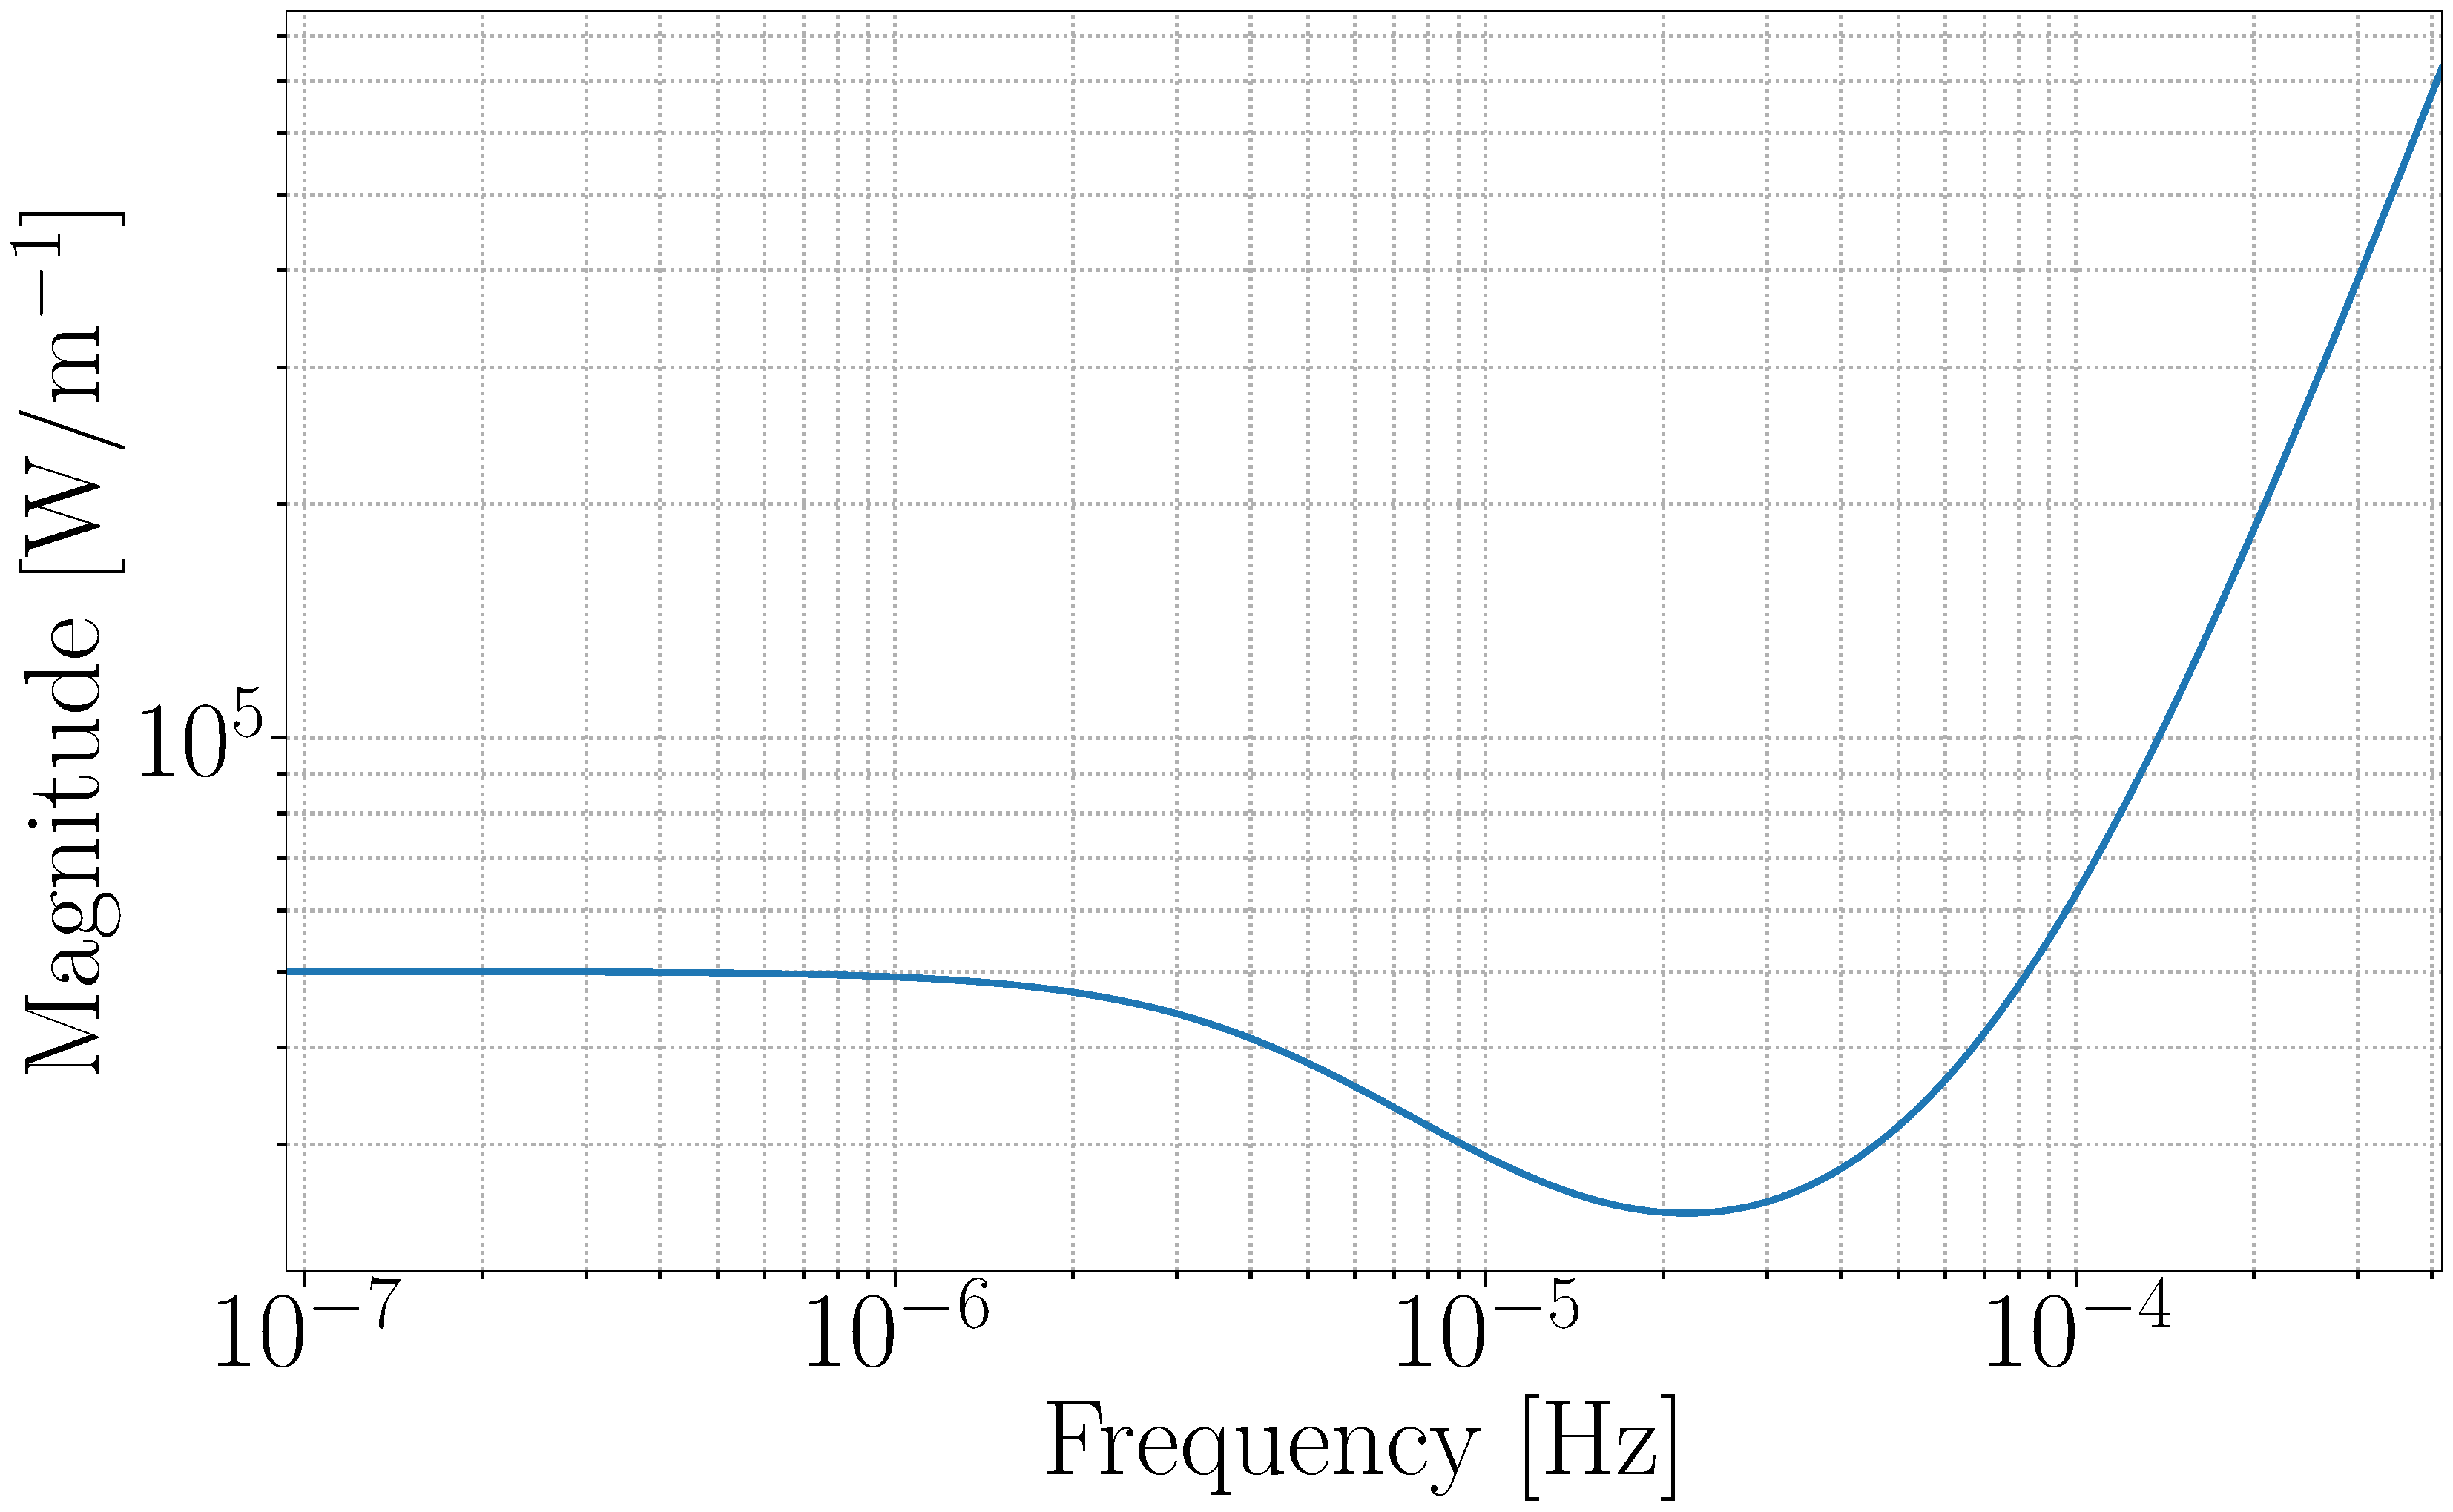
\includegraphics[width=\textwidth]{figs/TCS/IRHF/RH_inv_filt.pdf}
		\caption{Fitted zpk filter, inverted.}
	        \label{fig:rh_inv_filt}
    	    \end{figure}
	\item Apply correction filter $G(s)$ for stability and speed tuning ($H^{-1}(s)*G(s)$)
	    \begin{figure}[H]
		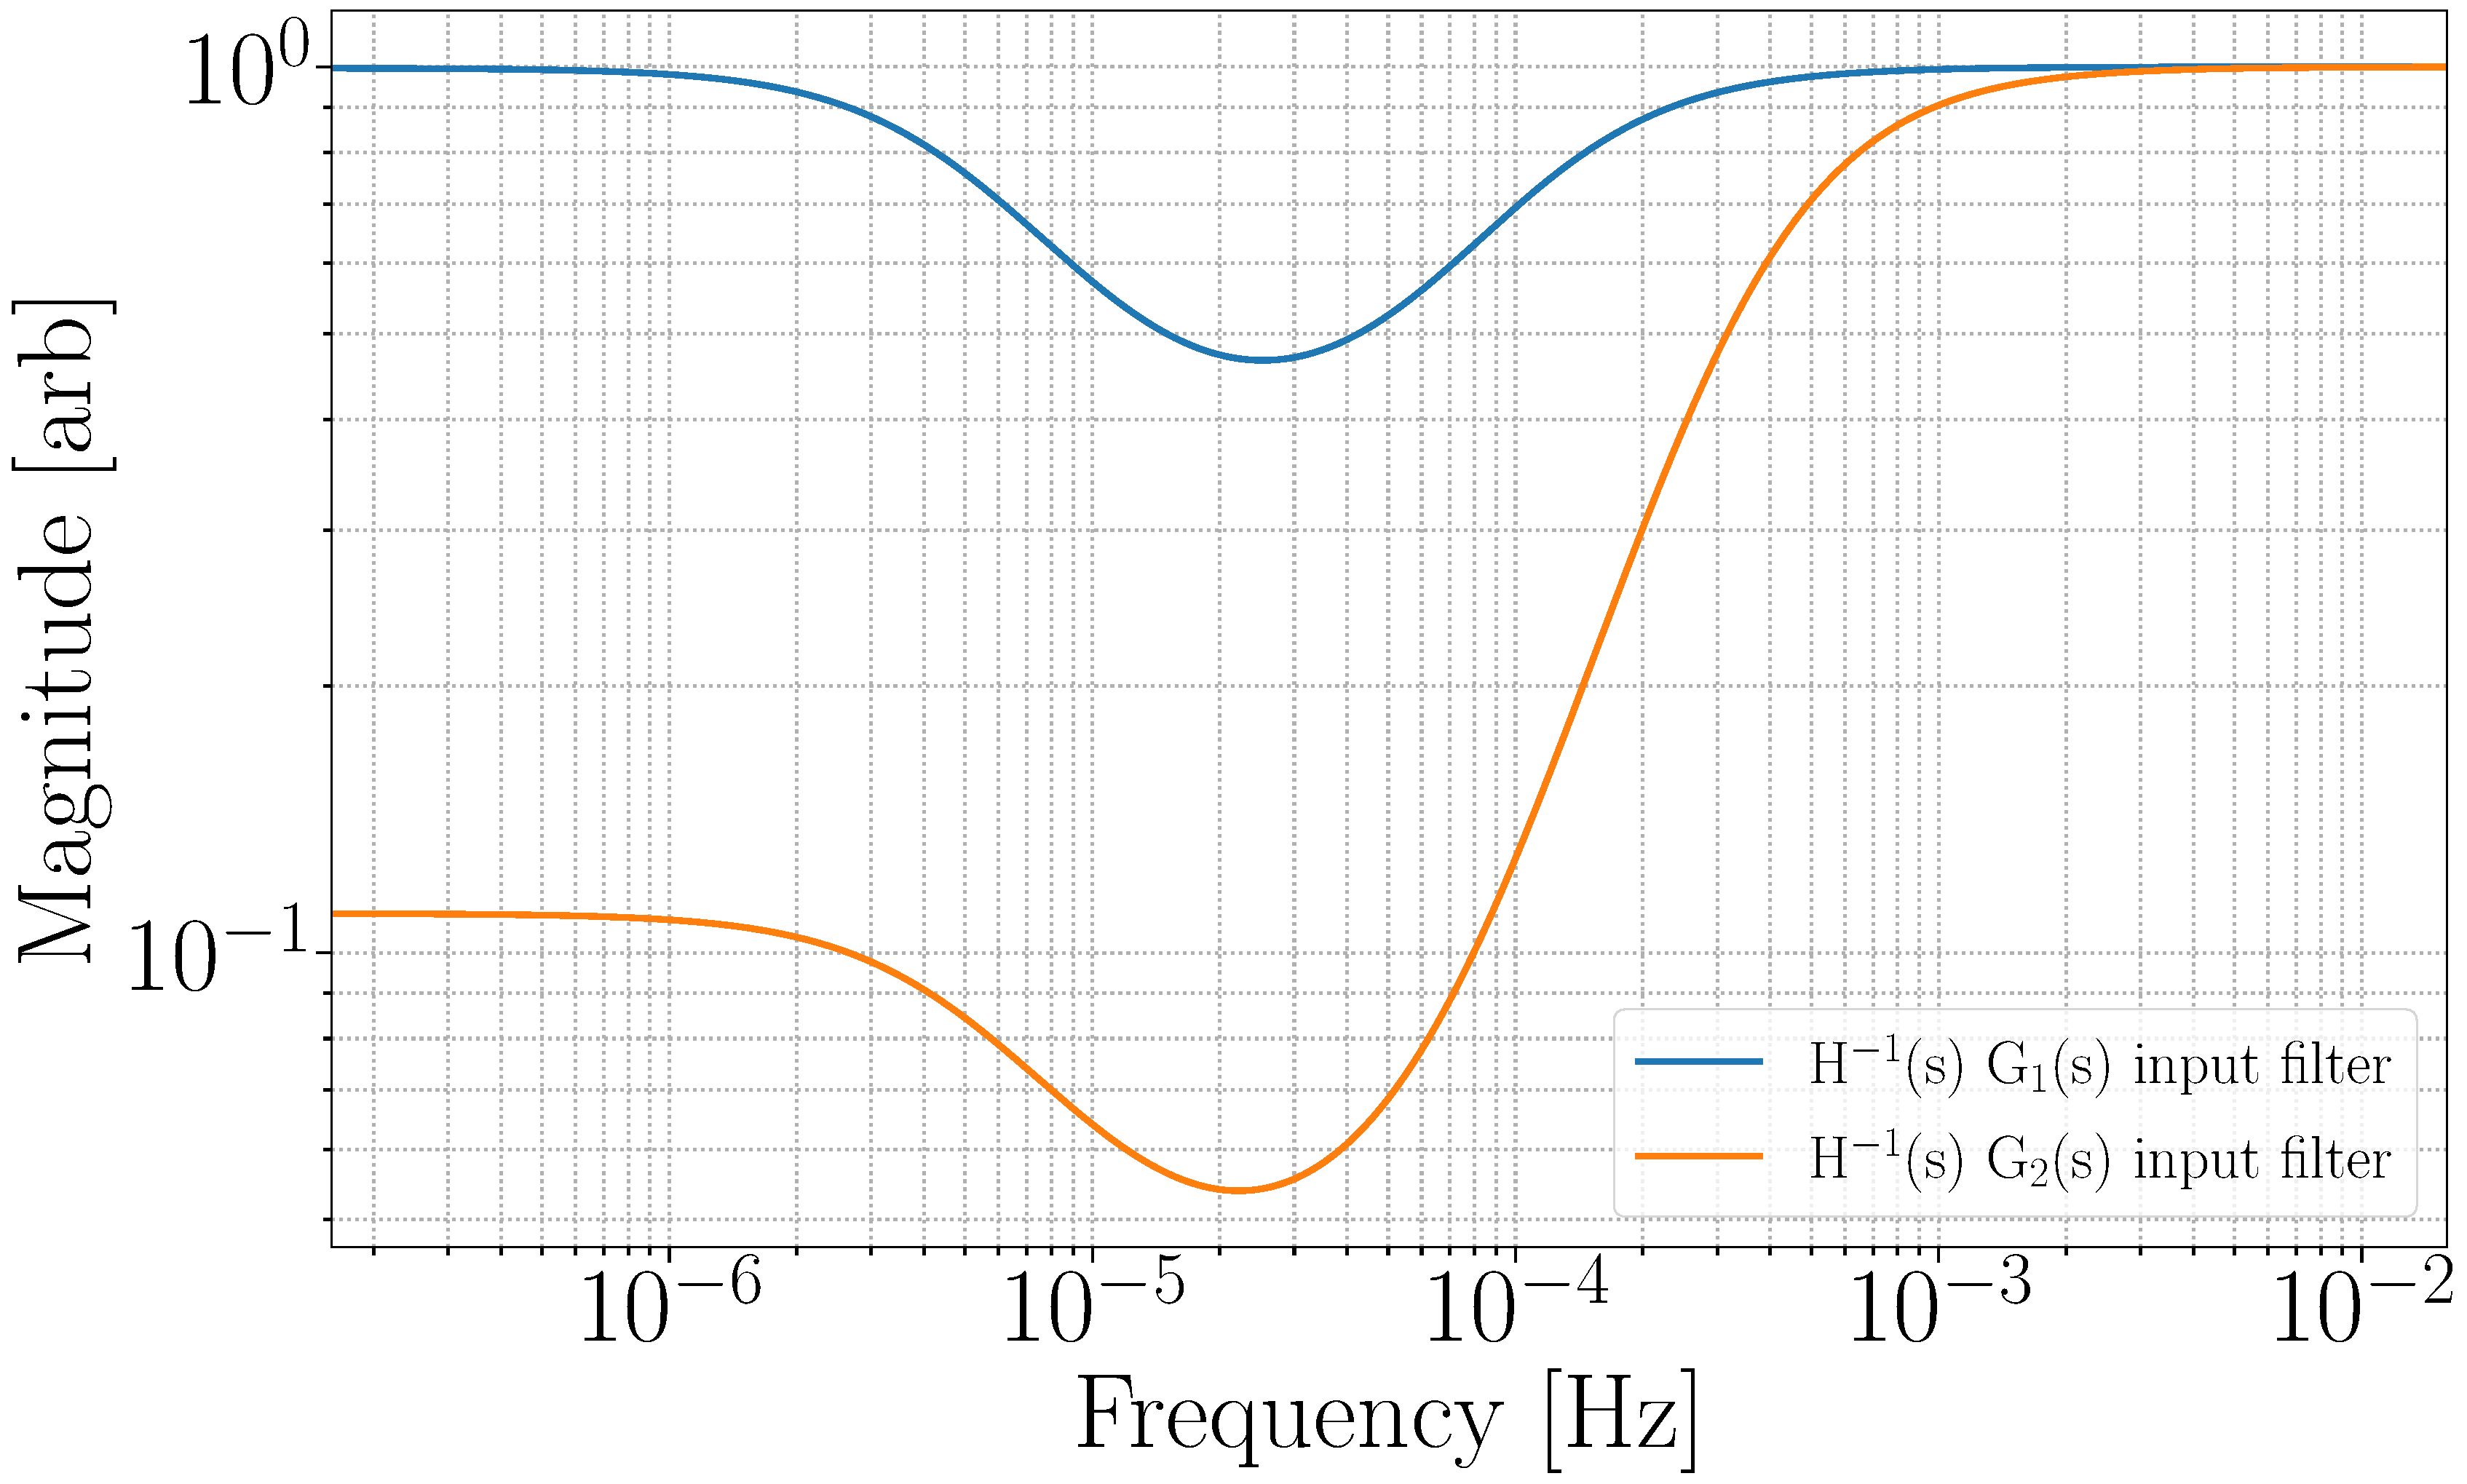
\includegraphics[width=\textwidth]{figs/TCS/IRHF/RH_input_filt_G1_G2.pdf}
		\caption{Fitted zpk filter to transient response of self heating COMSOL model.}
	        \label{fig:rh_input_filt}
    	    \end{figure}
\end{enumerate}


\subsection{code}
\begin{spacing}{1.2} \begin{lstlisting}[frame=single,language=Python]
import matplotlib
import matplotlib.pyplot as plt
import numpy as np
from scipy import signal
import h5py
import os

plt_style_dir = '../../../my_python/matplotlib/stylelib/'
if os.path.isdir(plt_style_dir) == True:
    plt.style.use(plt_style_dir + 'ppt2latex')
plt.rcParams["font.family"] = "Times New Roman"
\end{lstlisting} \end{spacing}

\begin{spacing}{1.2} \begin{lstlisting}[frame=single,language=Python]
# Establish default color array
prop_cycle = plt.rcParams['axes.prop_cycle']
colors = prop_cycle.by_key()['color']
lin_thickness=4
\end{lstlisting} \end{spacing}

\begin{spacing}{1.2} \begin{lstlisting}[frame=single,language=Python]
## Set figure saving directory
thesis_dir = '../doc/figures/python/'
thesis_dir='../../dissertation/figs/TCS/IRHF/'
\end{lstlisting} \end{spacing}

Generating / plotting plant filter

\begin{spacing}{1.2} \begin{lstlisting}[frame=single,language=Python]
ITMYRH_data = np.loadtxt('../data/ITMY_trend_10min_int_longer.dat')
t = np.arange(0,len(ITMYRH_data[:,0][2:]))*60.0*10.0
normalize = 3.13
print(len(t))
data_in = ITMYRH_data[:,1][2:]
b, a = signal.butter(2, .2)
#data_new = signal.filtfilt(b,a,data_in)
data_new = data_in
plt.figure()
ir = (data_new[1:] - data_new[:-1])/normalize
ir_new = ir
fig1 = plt.figure(figsize=(13,10))
plt.plot(t, data_new, label='Step response',linewidth=lin_thickness)
#plt.plot(t[:(len(t)-1)], ir, label= 'Impulse response')
plt.xlabel('time [s]')
plt.ylabel('Defocus [m$^{-1}$]')
#plt.legend(fontsize='medium')
plt.show()

Fs = 1/(t[2]-t[1])
#print(Fs)

[F,H]=signal.freqz(ir_new,1, worN=3000,whole=False) 
fig2 = plt.figure(figsize=(13,10))
plt.loglog(F*Fs/(2*np.pi), abs(H), label='Plant filter',linewidth=lin_thickness)
plt.ylabel('Magnitude [m$^{-1}$/W]')
plt.xlabel('Frequency [Hz]')
plt.legend()
plt.show()

print(max(ir_new))
\end{lstlisting} \end{spacing}

%\begin{figure}
%\centering
%\includegraphics{IRHF_w_self_heating_files/IRHF_w_self_heating_5_2.png}
%\caption{png}
%\end{figure}
%
%\begin{figure}
%\centering
%\includegraphics{IRHF_w_self_heating_files/IRHF_w_self_heating_5_3.png}
%\caption{png}
%\end{figure}

\begin{spacing}{1.2} \begin{lstlisting}[frame=single,language=Python]
adj_data = data_new + abs(min(data_new))
mod_data = np.concatenate([np.zeros((10,)), adj_data])
mod_t = np.arange(0,len(mod_data))*60.0*10.0/(3600)
mod_rh_inp = np.concatenate([np.ones((10,))*3.13, np.zeros(adj_data.shape)])
\end{lstlisting} \end{spacing}

\begin{spacing}{1.2} \begin{lstlisting}[frame=single,language=Python]
fig, ax1 = plt.subplots() 

ax1.set_xlabel('time [hr]') 
ax1.set_ylabel('Primary-axis') 
ax1.plot(mod_t, mod_rh_inp,'--',linewidth=lin_thickness, color = colors[0]) 
ax1.tick_params(axis='y', labelcolor=colors[0])
ax1.set_ylabel('RH power [W]', color=colors[0])
#ax1.grid(b=False,which='minor',linestyle='--')
#ax1.grid(b=False,which='major',linestyle='--')
ax1.minorticks_off()
ax1.set_xlim([0,mod_t[-1]])
ax1.set_ylim([-.01,4])

ax2 = ax1.twinx() 
ax2.plot(mod_t, mod_data,linewidth=lin_thickness, color = colors[1])
ax2.set_ylabel('Defocus [m$^{-1}$]',color= colors[1])
##plt.grid(b=True,which='minor',linestyle='--')
##plt.grid(b=True,which='major',linestyle='--')
##plt.minorticks_on()
ax2.set_xlim([0,mod_t[-1]])
ax2.tick_params(axis='y', labelcolor=colors[1])
ax2.ticklabel_format(style='sci', axis='y',scilimits=(0,-5))

ax2.set_ylim([-.003e-4,1.2e-4])

fig.savefig(thesis_dir + 'Meas_response.pdf', dpi=300, format='pdf', bbox_inches='tight')
\end{lstlisting} \end{spacing}

%\begin{figure}
%\centering
%\includegraphics{IRHF_w_self_heating_files/IRHF_w_self_heating_8_0.png}
%\caption{png}
%\end{figure}

\begin{spacing}{1.2} \begin{lstlisting}[frame=single,language=Python]
print('Only plots up to the nyqist frequency: {} Hz'.format(F[-1]*Fs/(2*np.pi)))
\end{lstlisting} \end{spacing}

\begin{spacing}{1.2} \begin{lstlisting}
Only plots up to the nyqist frequency: 0.0008330555555555556 Hz
\end{lstlisting} \end{spacing}

\begin{spacing}{1.2} \begin{lstlisting}[frame=single,language=Python]
zeros = 5.0e-6
fit_zeros = -2.0*np.pi*zeros
poles = np.array([1.3e-5, 5.0e-5 ,9.5e-5])
fit_poles = -2.0*np.pi*poles

k = 1 #This gain is not initally correct

s1 = signal.ZerosPolesGain(fit_zeros, fit_poles, k)
F_2, H_2 = signal.freqresp(s1, F*(Fs/2.0))

#[F_2,H_2] = signal.freqs(b_2, a_2)
k_new = abs(H[0])/abs(H_2[0])

plt.loglog(F_2/(2*np.pi), abs(H_2)*k_new, label='Fitted zpk filter',linewidth=lin_thickness)
plt.loglog(F/(2*np.pi)*Fs, abs(H), label='Measured (step response) filter',linewidth=lin_thickness)
plt.ylabel('Magnitude [W/m$^{-1}$]')
plt.xlabel('Frequency [Hz]')
plt.legend()
#plt.title('RH plant filter (H(s))')
plt.xlim([0,(F[-1]/(2*np.pi)*Fs)])
print(k_new) #Spit out the new gain
##plt.grid(b=True,which='minor')
##plt.grid(b=True,which='major')
##plt.minorticks_on()

model_zpk = signal.ZerosPolesGain(fit_zeros, fit_poles,k_new)

plt.savefig(thesis_dir+'RH_plant_filter_fit.pdf',bbox_inches = 'tight')
\end{lstlisting} \end{spacing}

%\begin{figure}
%\centering
%\includegraphics{IRHF_w_self_heating_files/IRHF_w_self_heating_10_2.png}
%\caption{png}
%\end{figure}

\begin{spacing}{1.2} \begin{lstlisting}[frame=single,language=Python]
model_zpk
\end{lstlisting} \end{spacing}

\begin{spacing}{1.2} \begin{lstlisting}[frame=single]
ZerosPolesGainContinuous(
array([-3.14159265e-05]),
array([-8.16814090e-05, -3.14159265e-04, -5.96902604e-04]),
9.729529652779821e-12,
dt: None
)
\end{lstlisting} \end{spacing}

\noindent Now to invert the plant filter (just swapping the poles and the zeros and inverting gain)
(H\(^{-1}\)(s))

\begin{spacing}{1.2} \begin{lstlisting}[frame=single,language=Python]
inv_model = signal.ZerosPolesGain(fit_poles, fit_zeros,1/k_new)
F_3, H_3 = signal.freqresp(inv_model, F*(Fs/2.0))
fig4 = plt.figure()
plt.loglog(F_3/(2*np.pi), abs(H_3), label='Fitted zpk Filter',linewidth=lin_thickness)
plt.ylabel('Magnitude [W/m$^{-1}$]')
plt.xlabel('Frequency [Hz]')
#plt.title('RH inverse filter ([H(s)]$^{-1}$)')
plt.xlim([0, F_3[-1]/(2*np.pi)])
###plt.grid(b=True,which='minor',linestyle='--')
##plt.grid(b=True,which='major',linestyle='--')
#plt.minorticks_on()
plt.savefig(thesis_dir+'RH_inv_filt.pdf',bbox_inches = 'tight')
\end{lstlisting} \end{spacing}

%\begin{figure}
%\centering
%\includegraphics{IRHF_w_self_heating_files/IRHF_w_self_heating_13_1.png}
%\caption{png}
%\end{figure}

\noindent Stabilize the high frequencies to DC (Generating H\(^{-1}\) (s) * G\(_{n}\)(s))

\noindent Will also attempt to reduce the time constant

\begin{spacing}{1.2} \begin{lstlisting}[frame=single,language=Python]
#pole_test = .0001113 + 1e-4
Hinv_G_1_filt = signal.ZerosPolesGain(fit_poles, [fit_zeros,-2.0*np.pi*.0001113129672, -2.0*np.pi*.0001113129672],1)
pole_shift = 3
Hinv_G_2_filt = signal.ZerosPolesGain(fit_poles, [fit_zeros,-2.0*np.pi*.0001113129672*pole_shift, -2.0*np.pi*.0001113129672*pole_shift],1)

## Plotting
freq = np.arange(10e-7,10e-2,1e-7)
F_4, H_4 = signal.freqresp(Hinv_G_1_filt,freq)
F_5, H_5 = signal.freqresp(Hinv_G_2_filt,freq)

fig5= plt.figure()
plt.loglog(F_4/(2*np.pi), abs(H_4), label='RH input filter',linewidth=lin_thickness)
#plt.loglog(F_5/(2*np.pi), abs(H_5), label='Livingston filter',linewidth=lin_thickness)
#plt.legend(fontsize='xx-large')
plt.xlim([F_4[0]/(2*np.pi),F_4[-1]/(2*np.pi)])
#plt.grid(b=True,which='minor',linestyle='--')
#plt.grid(b=True,which='major',linestyle='--')
##plt.minorticks_on()
plt.ylabel('Magnitude [arb]')
plt.xlabel('Frequency [Hz]')
#plt.title('Real-time RH filter [H(s)]$^{-1*}$', **title_font)

plt.savefig(thesis_dir+'RH_input_filt.pdf',bbox_inches='tight')
\end{lstlisting} \end{spacing}

%\begin{figure}
%\centering
%\includegraphics{IRHF_w_self_heating_files/IRHF_w_self_heating_15_0.png}
%\caption{png}
%\end{figure}

\begin{spacing}{1.2} \begin{lstlisting}[frame=single,language=Python]
Hinv_G_1_filt
\end{lstlisting} \end{spacing}

\begin{spacing}{1.2} \begin{lstlisting}[frame=single]
ZerosPolesGainContinuous(
array([-8.16814090e-05, -3.14159265e-04, -5.96902604e-04]),
array([-3.14159265e-05, -6.99400000e-04, -6.99400000e-04]),
1,
dt: None
)
\end{lstlisting} \end{spacing}

\begin{spacing}{1.2} \begin{lstlisting}[frame=single,language=Python]
Hinv_G_2_filt
\end{lstlisting} \end{spacing}

\begin{spacing}{1.2} \begin{lstlisting}[frame=single]
ZerosPolesGainContinuous(
array([-8.16814090e-05, -3.14159265e-04, -5.96902604e-04]),
array([-3.14159265e-05, -2.09820000e-03, -2.09820000e-03]),
1,
dt: None
)
\end{lstlisting} \end{spacing}

\begin{spacing}{1.2} \begin{lstlisting}[frame=single,language=Python]
fig79= plt.figure()
plt.loglog(F_4/(2*np.pi), abs(H_4), label='G$_1$(s) input filter',linewidth=lin_thickness)
plt.loglog(F_5/(2*np.pi), abs(H_5), label='G$_2$(s) input filter',linewidth=lin_thickness)
plt.legend()
plt.xlim([F_4[0]/(2*np.pi),F_4[-1]/(2*np.pi)])
#plt.grid(b=True,which='minor',linestyle='--')
#plt.grid(b=True,which='major',linestyle='--')
#plt.minorticks_on()
plt.ylabel('Magnitude [arb]')
plt.xlabel('Frequency [Hz]')
#plt.title('Real-time RH filter [H(s)]$^{-1*}$', **title_font)

plt.savefig(thesis_dir+'RH_input_filt_G1_G2.pdf',bbox_inches='tight')
\end{lstlisting} \end{spacing}

%\begin{figure}
%\centering
%\includegraphics{IRHF_w_self_heating_files/IRHF_w_self_heating_18_0.png}
%\caption{png}
%\end{figure}

\noindent COMSOL self heating filter

\noindent Import COMSOL self heating data

\begin{spacing}{1.2} \begin{lstlisting}[frame=single,language=Python]
COM_data = np.loadtxt('../data/1W_self_heating_defocus_doublepass.txt')
t_com = COM_data[:,0]*3600
defocus = COM_data[:,1]/max(COM_data[:,1])
\end{lstlisting} \end{spacing}

\begin{spacing}{1.2} \begin{lstlisting}[frame=single,language=Python]
fig6 = plt.figure()
plt.plot(t_com/3600,defocus,linewidth=lin_thickness)
plt.title('COMSOL self heating time series')
plt.xlabel('time [hrs]')
plt.ylabel('defocus [arb]')
max(defocus)
\end{lstlisting} \end{spacing}

%\begin{figure}
%\centering
%\includegraphics{IRHF_w_self_heating_files/IRHF_w_self_heating_22_1.png}
%\caption{png}
%\end{figure}

\begin{spacing}{1.2} \begin{lstlisting}[frame=single,language=Python]
ir_com  = (defocus[1:] - defocus[:-1])
t_ir = t_com[:((len(t_com)-1))]
\end{lstlisting} \end{spacing}

\begin{spacing}{1.2} \begin{lstlisting}[frame=single,language=Python]
[F_ir,H_ir]=signal.freqz(ir_com, 1, worN=3000,whole=False) 
Fs_com =1/(t_com[1]-t_com[0])
\end{lstlisting} \end{spacing}

\begin{spacing}{1.2} \begin{lstlisting}[frame=single,language=Python]
zeros_com = np.array([.9e-3,.3e-3])
fit_zeros_com = -2.0*np.pi*zeros_com
poles_com = np.array([.25e-3,.25e-3,1.6e-3])
fit_poles_com = -2.0*np.pi*poles_com

k_com =1 #This gain is not initally correct

zpk_com = signal.ZerosPolesGain(fit_zeros_com, fit_poles_com, k_com)
F_com, H_com = signal.freqresp(zpk_com, F_ir*(Fs_com/2.0))
k_new_com = abs(H_ir[0])/abs(H_ir[0]*H_com[0])

fig6 = plt.figure()
plt.loglog(F_com/(2*np.pi), abs(H_com)*k_new_com, label='Fitted zpk Filter',linewidth=lin_thickness)
plt.loglog(F_ir*Fs_com/(2*np.pi), abs(H_ir)/abs(H_ir[0]), label='Plant filter',linewidth=lin_thickness)
plt.ylabel('Magnitude [arb]')
plt.xlabel('Frequency [Hz]')
plt.title('Self Heating filter')
\end{lstlisting} \end{spacing}

%\begin{figure}
%\centering
%\includegraphics{IRHF_w_self_heating_files/IRHF_w_self_heating_25_1.png}
%\caption{png}
%\end{figure}

\begin{spacing}{1.2} \begin{lstlisting}[frame=single,language=Python]
G_2 = signal.ZerosPolesGain(fit_zeros_com, fit_poles_com, k_new_com)
unit_step_testing = np.zeros(np.shape(t_com))
unit_step_testing[t_com>0] = 1
[ _ ,y_self_test, _] = signal.lsim(G_2, unit_step_testing, t_com)
\end{lstlisting} \end{spacing}

\begin{spacing}{1.2} \begin{lstlisting}[frame=single,language=Python]
fig7= plt.figure()
plt.plot(t_com/3600,defocus,label='measured',linewidth=lin_thickness)
plt.plot(t_com/3600,y_self_test,label='fit',linewidth=lin_thickness)
plt.title('Self heating time series (fit vs measured)')
plt.legend()
\end{lstlisting} \end{spacing}

%\begin{figure}
%\centering
%\includegraphics{IRHF_w_self_heating_files/IRHF_w_self_heating_27_1.png}
%\caption{png}
%\end{figure}

\subsubsection*{Generating time series}

\noindent Step input time series

\begin{spacing}{1.2} \begin{lstlisting}[frame=single,language=Python]
unit_step = np.zeros((t.shape[0]*30))
t_new = np.arange(0,len(unit_step))*60.0*1.0
## Generating simulated response
unit_step[t_new>9000] = 1
[t_mod_new,y_mod_sim,xout] = signal.lsim(model_zpk, unit_step, t_new)
\end{lstlisting} \end{spacing}


\noindent Conditioned input time series

\begin{spacing}{1.2} \begin{lstlisting}[frame=single,language=Python]
unit_step2 = np.zeros((t.shape[0]*30))
unit_step2[t_new>(9000)] = pole_shift**2

[ _ ,y_inp_inv_L, _] = signal.lsim(Hinv_G_2_filt, unit_step2, t_new)
[ _ ,y_inp_inv_H, _] = signal.lsim(Hinv_G_1_filt, unit_step, t_new)
[ _ ,y_mod_sim_inv_L, _] = signal.lsim(model_zpk, y_inp_inv_L, t_new)
[ _ ,y_mod_sim_inv_H, _] = signal.lsim(model_zpk, y_inp_inv_H, t_new)
\end{lstlisting} \end{spacing}


\noindent Self heating time series

\begin{spacing}{1.2} \begin{lstlisting}[frame=single,language=Python]
unit_step3 = np.zeros((t.shape[0]*30))
t_offset =0
unit_step3[t_new>(9000+t_offset)] = 1
\end{lstlisting} \end{spacing}

\begin{spacing}{1.2} \begin{lstlisting}[frame=single,language=Python]
[ _ ,y_sh_resp, _] = signal.lsim(G_2, unit_step3, t_new)
\end{lstlisting} \end{spacing}

\noindent Basic Performance

\begin{spacing}{1.2} \begin{lstlisting}[frame=single,language=Python]
fig = plt.figure()
plt.subplot(211)
plt.plot(t_new/3600, unit_step,linewidth = lin_thickness,label='RH step input')
plt.plot(t_new/3600, y_inp_inv_H,'--', linewidth = lin_thickness,color = 'red', label='RH filtered input')
plt.ylabel('RH power [W]')
#plt.title('RH step input vs. Filtered input')
plt.legend()
plt.xlim([0, t_new[-1]/3600])
#plt.grid(b=True,which='minor',linestyle='--')
#plt.grid(b=True,which='major',linestyle='--')
#plt.minorticks_on()
plt.subplot(212)
plt.plot(t_new/3600,-y_mod_sim, linewidth = lin_thickness,label = 'RH step input')
plt.plot(t_new/3600,-y_mod_sim_inv_H,'--', linewidth = lin_thickness,color='red',label ='RH filtered input')
plt.ylabel('Defocus [m$^{-1}$]')
plt.xlabel('time [hr]')
#plt.legend()
plt.xlim([0, t_new[-1]/3600])
#plt.grid(b=True,which='minor',linestyle='--')
#plt.grid(b=True,which='major',linestyle='--')
#plt.minorticks_on()
plt.ticklabel_format(style='sci', axis='y',scilimits=(0,-5))
fig.savefig(thesis_dir+'IRHF_step_vs_filt_step.pdf',bbox_inches='tight')
\end{lstlisting} \end{spacing}

%\begin{figure}
%\centering
%\includegraphics{IRHF_w_self_heating_files/IRHF_w_self_heating_37_0.png}
%\caption{png}
%\end{figure}


\noindent All curves together

\begin{spacing}{1.2} \begin{lstlisting}[frame=single,language=Python]
fig = plt.figure()
plt.subplot(211)
plt.plot(t_new/3600, unit_step,linewidth = lin_thickness,label='RH unfiltered step input')
plt.plot(t_new/3600, y_inp_inv_L,'--', linewidth = lin_thickness, color = 'green',label='RH conditioned input (G$_{1}$(s))')
plt.plot(t_new/3600, y_inp_inv_H,'--', linewidth = lin_thickness,color = 'red', label='RH conditioned input (G$_{2}$(s)')
plt.ylabel('RH power [W]')
plt.title('RH filtered response w/ self-heating')
plt.legend(fontsize='medium')
plt.xlim([0,20])
plt.subplot(212)
plt.plot(t_new/3600,-y_mod_sim, linewidth = lin_thickness,label = 'RH unfiltered step input')
plt.plot(t_new/3600,y_sh_resp*20e-6, linewidth = lin_thickness,color='orange',label ='self heating')
plt.plot(t_new/3600,-y_mod_sim_inv_L,'--', linewidth = lin_thickness,color='green',label ='RH conditioned input (G$_{1}$(s))')
plt.plot(t_new/3600,-y_mod_sim_inv_H,'--', linewidth = lin_thickness,color='red',label ='RH conditioned input (G$_{2}$(s)')
plt.plot(t_new/3600,y_sh_resp*20e-6 -y_mod_sim_inv_L,linewidth = lin_thickness,label='self heating + RH conditioned input (G$_{1}$(s)',color='purple')
plt.plot(t_new/3600,y_sh_resp*20e-6 -y_mod_sim_inv_H,linewidth = lin_thickness,label='self heating + RH conditioned input (G$_{2}$(s))',color='magenta')
plt.ylabel('Defocus [m$^{-1}$]')
plt.xlabel('time [hr]')
plt.legend(fontsize='medium')
plt.xlim([0,20])
fig.savefig(thesis_dir+'IRHF_compare_self_w_filter_compare.pdf',bbox_inches='tight')
\end{lstlisting} \end{spacing}

%\begin{figure}
%\centering
%\includegraphics{IRHF_w_self_heating_files/IRHF_w_self_heating_39_0.png}
%\caption{png}
%\end{figure}

\begin{spacing}{1.2} \begin{lstlisting}[frame=single,language=Python]
fig8 = plt.figure()
plt.rc('font', size=25)
plt.plot(t_new/3600,y_sh_resp*20e-6, linewidth = lin_thickness,color='orange',label ='self heating with no RH')
plt.plot(t_new/3600,y_sh_resp*20e-6 -y_mod_sim,linewidth = lin_thickness,label='self heating + RH unfiltered input',color='purple')
plt.plot(t_new/3600,y_sh_resp*20e-6 -y_mod_sim_inv_H,'--',linewidth = lin_thickness,label='self heating + RH filtered input (H$^{-1}$(s)*G$_{1}$(s))',color='red')
plt.plot(t_new/3600,y_sh_resp*20e-6 -y_mod_sim_inv_L,'--',linewidth = lin_thickness,label='self heating + RH filtered input (H$^{-1}$(s)*G$_{2}$(s))',color='green')
plt.ylabel('Defocus [m$^{-1}$]')
plt.xlabel('time [hr]')
plt.ticklabel_format(style='sci', axis='y',scilimits=(0,-5))
plt.xlim([0,20])
plt.legend(loc='upper right',bbox_to_anchor=(1.0,.95))
fig8.savefig(thesis_dir+'IRHF_compare_w_self.pdf',bbox_inches='tight')
\end{lstlisting} \end{spacing}

%\begin{figure}
%\centering
%\includegraphics{IRHF_w_self_heating_files/IRHF_w_self_heating_40_0.png}
%\caption{png}
%\end{figure}

\noindent Set RH upper limit

\begin{spacing}{1.2} \begin{lstlisting}[frame=single,language=Python]
upper_lim = np.ones(np.shape(t_new))*40
\end{lstlisting} \end{spacing}

\begin{spacing}{1.2} \begin{lstlisting}[frame=single,language=Python]
fig9= plt.figure(figsize=(25,20))
plt.rc('font', size=30)
plt.subplot(211)
plt.plot(t_new/3600, unit_step,linewidth = lin_thickness,label='Step input', color= 'purple')
plt.plot(t_new/3600, y_inp_inv_L,'--', linewidth = lin_thickness, color = 'green',label='Filtered input')
#plt.plot(t_new/3600, upper_lim,':',linewidth = lin_thickness, color='magenta', label='RH upper limit')
#plt.plot(t_new/3600, y_inp_inv_H,'--', linewidth = lin_thickness,color = 'red', label='Filtered input (H$^{-1}$(s)G$_{1}$(s))')
#plt.minorticks_on()
#plt.grid(b=True,which='minor',linestyle='--')
#plt.grid(b=True,which='major',linestyle='--')
plt.ylabel('RH power [W]')
plt.xlim([0,20])
#plt.title('RH responses')
plt.legend(fontsize='large')
plt.subplot(212)
plt.ylabel('Defocus [m$^{-1}$]')
plt.plot(t_new/3600,y_sh_resp*20e-6, linewidth = lin_thickness,color='orange',label ='central heating with no RH')
plt.plot(t_new/3600,(y_sh_resp*20e-6 -y_mod_sim),linewidth = lin_thickness,label='central heating + RH w/ step input',color='purple')
plt.plot(t_new/3600,(y_sh_resp*20e-6 -y_mod_sim_inv_L),'--',linewidth = lin_thickness,label='central heating + RH w/ filtered input',color='green')
#plt.plot(t_new/3600,-y_mod_sim, linewidth = lin_thickness,label = 'Unfiltered step input',color='purple')
#plt.plot(t_new/3600,y_sh_resp*20e-6-y_mod_sim_inv_L,'--', linewidth = lin_thickness,color='green',label ='Filtered input (H$^{-1}$(s)G$_{2}$(s))')
#plt.plot(t_new/3600,-y_mod_sim_inv_H,'--', linewidth = lin_thickness,color='red',label ='Filtered input (H$^{-1}$(s)G$_{1}$(s))')
#plt.minorticks_on()
#plt.grid(b=True,which='minor',linestyle='--')
#plt.grid(b=True,which='major',linestyle='--')
plt.xlabel('time [hr]')
plt.ticklabel_format(style='sci', axis='y',scilimits=(0,-5))
plt.legend(loc='upper right', bbox_to_anchor=(1.0,.95),fontsize='large')
plt.xlim([0,20])

fig9.savefig(thesis_dir+'IRHF_compare_filts_PI_paper.pdf',bbox_inches='tight')
\end{lstlisting} \end{spacing}

%\begin{figure}
%\centering
%\includegraphics{IRHF_w_self_heating_files/IRHF_w_self_heating_43_0.png}
%\caption{png}
%\end{figure}

\begin{spacing}{1.2} \begin{lstlisting}[frame=single,language=Python]
fig9= plt.figure(figsize=(25,20))
plt.rc('font', size=30)
plt.subplot(211)
plt.plot(t_new/3600, unit_step,linewidth = lin_thickness,label='Step input', color= 'purple')
#plt.plot(t_new/3600, upper_lim,':',linewidth = lin_thickness, color='magenta', label='RH upper limit')
plt.plot(t_new/3600, y_inp_inv_L,'--', linewidth = lin_thickness, color = 'green',label='Filtered input(H$^{-1}$(s)G$_{2}$(s))')
plt.plot(t_new/3600, y_inp_inv_H,'--', linewidth = lin_thickness,color = 'red', label='Filtered input (H$^{-1}$(s)G$_{1}$(s))')
#plt.minorticks_on()
#plt.grid(b=True,which='minor',linestyle='--')
#plt.grid(b=True,which='major',linestyle='--')
plt.ylabel('RH power [W]')
plt.xlim([0,20])
#plt.title('RH responses')
plt.legend(fontsize='large')
plt.subplot(212)
plt.ylabel('Defocus [m$^{-1}$]')
plt.plot(t_new/3600,y_sh_resp*20e-6, linewidth = lin_thickness,color='orange',label ='self heating with no RH')
plt.plot(t_new/3600,(y_sh_resp*20e-6 -y_mod_sim),linewidth = lin_thickness,label='self heating + RH w/ step input',color='purple')
#plt.plot(t_new/3600,(y_sh_resp*20e-6 -y_mod_sim_inv_L),'--',linewidth = lin_thickness,label='self heating + RH w/ filtered input',color='green')
#plt.plot(t_new/3600,-y_mod_sim, linewidth = lin_thickness,label = 'Unfiltered step input',color='purple')
plt.plot(t_new/3600,(y_sh_resp*20e-6-y_mod_sim_inv_L),'--', linewidth = lin_thickness,color='green',label ='Filtered input (H$^{-1}$(s)G$_{2}$(s))')
plt.plot(t_new/3600,(y_sh_resp*20e-6-y_mod_sim_inv_H),'--', linewidth = lin_thickness,color='red',label ='Filtered input (H$^{-1}$(s)G$_{1}$(s))')
#plt.minorticks_on()
#plt.grid(b=True,which='minor',linestyle='--')
#plt.grid(b=True,which='major',linestyle='--')
plt.xlabel('time [hr]')
plt.ticklabel_format(style='sci', axis='y',scilimits=(0,-5))
plt.legend(loc='upper right', bbox_to_anchor=(1.0,.97),fontsize='large')
plt.xlim([0,20])

fig9.savefig(thesis_dir+'IRHF_compare_filts.pdf',bbox_inches='tight')
fig9.savefig(thesis_dir+'IRHF_compare_filts.pdf',bbox_inches='tight')
\end{lstlisting} \end{spacing}

%\begin{figure}
%\centering
%\includegraphics{IRHF_w_self_heating_files/IRHF_w_self_heating_44_0.png}
%\caption{png}
%\end{figure}

\begin{spacing}{1.2} \begin{lstlisting}[frame=single,language=Python]
fig9= plt.figure(figsize=(17,15))
plt.rc('font', size=25)
plt.subplot(211)
plt.plot(t_new/3600, unit_step,linewidth = lin_thickness,label='Step input', color= 'purple')
plt.plot(t_new/3600, y_inp_inv_L,'--', linewidth = lin_thickness, color = 'green',label='Filtered input (H$^{-1}$(s)G$_{1}$(s))')
#plt.plot(t_new/3600, upper_lim,':',linewidth = lin_thickness, color='magenta', label='RH upper limit')
plt.plot(t_new/3600, y_inp_inv_H,'--', linewidth = lin_thickness,color = 'red', label='Filtered input (H$^{-1}$(s)G$_{2}$(s))')
#plt.minorticks_on()
#plt.grid(b=True,which='minor',linestyle='--')
#plt.grid(b=True,which='major',linestyle='--')
plt.ylabel('RH power [W]')
plt.xlim([0,t_new[-1]/3600])
#plt.title('RH responses')
plt.legend(fontsize='medium')
plt.subplot(212)
plt.ylabel('Defocus [m$^{-1}$]')
plt.plot(t_new/3600,y_sh_resp*20e-6, linewidth = lin_thickness,color='orange',label ='self heating w/ no RH')
plt.plot(t_new/3600,y_sh_resp*20e-6 -y_mod_sim,linewidth = lin_thickness,label='self heating + step input',color='purple')
plt.plot(t_new/3600,y_sh_resp*20e-6 -y_mod_sim_inv_L,'--',linewidth = lin_thickness,label='self heating + filtered input (H$^{-1}$(s)G$_{1}$(s))',color='green')
plt.plot(t_new/3600,y_sh_resp*20e-6 -y_mod_sim_inv_H,'--',linewidth = lin_thickness,label='self heating + filtered input (H$^{-1}$(s)G$_{2}$(s))',color='red')
#plt.plot(t_new/3600,-y_mod_sim, linewidth = lin_thickness,label = 'Unfiltered step input',color='purple')
#plt.plot(t_new/3600,-y_mod_sim_inv_L,'--', linewidth = lin_thickness,color='green',label ='Filtered input (H$^{-1}$(s)G$_{2}$(s))')
#plt.plot(t_new/3600,-y_mod_sim_inv_H,'--', linewidth = lin_thickness,color='red',label ='Filtered input (H$^{-1}$(s)G$_{1}$(s))')
#plt.minorticks_on()
#plt.grid(b=True,which='minor',linestyle='--')
#plt.grid(b=True,which='major',linestyle='--')
plt.xlabel('time [hr]')
plt.xlim([0,t_new[-1]/3600])
plt.ticklabel_format(style='sci', axis='y',scilimits=(0,-5))
plt.legend(loc='upper right', bbox_to_anchor=(1.0,.97),fontsize='medium')

fig9.savefig(thesis_dir+'IRHF_compare_filts.pdf',bbox_inches='tight')
\end{lstlisting} \end{spacing}

%\begin{figure}
%\centering
%\includegraphics{IRHF_w_self_heating_files/IRHF_w_self_heating_45_0.png}
%\caption{png}
%\end{figure}

\begin{spacing}{1.2} \begin{lstlisting}[frame=single,language=Python]
fig = plt.figure(figsize=(17,15))
plt.subplot(311)
plt.plot(t_new/3600, unit_step,linewidth = lin_thickness,label='Unfiltered step input')
plt.plot(t_new/3600, y_inp_inv_L,'--', linewidth = lin_thickness, color = 'green',label='Conditioned input (G$_{1}$(s))')
plt.plot(t_new/3600, y_inp_inv_H,'--', linewidth = lin_thickness,color = 'red', label='Conditioned input (G$_{1}$(s))')
plt.ylabel('RH power [W]')
#plt.title('RH responses')
plt.legend(fontsize='small')
plt.subplot(312)
plt.ylabel('RH Defocus [m$^{-1}$]')
plt.plot(t_new/3600,-y_mod_sim, linewidth = lin_thickness,label = 'Unfiltered step input')
plt.plot(t_new/3600,-y_mod_sim_inv_L,'--', linewidth = lin_thickness,color='green',label ='Conditioned input (G$_{2}$(s))')
plt.plot(t_new/3600,-y_mod_sim_inv_H,'--', linewidth = lin_thickness,color='red',label ='Conditioned input (G$_{1}$(s))')
plt.legend(fontsize='x-small',loc='upper right')
plt.subplot(313)
plt.plot(t_new/3600,y_sh_resp*20e-6, linewidth = lin_thickness,color='orange',label ='Self heating')
plt.plot(t_new/3600,y_sh_resp*20e-6 -y_mod_sim,linewidth = lin_thickness,label='Self heating + RH unfiltered input',color='C0')
plt.plot(t_new/3600,y_sh_resp*20e-6 -y_mod_sim_inv_H,'--',linewidth = lin_thickness,label='Self heating + RH conditioned input (G$_{1}$(s))',color='red')
plt.plot(t_new/3600,y_sh_resp*20e-6 -y_mod_sim_inv_L,'--',linewidth = lin_thickness,label='Self heating + RH conditioned input (G$_{2}$(s))',color='green')
plt.ylabel('Total Defocus [m$^{-1}$]')
plt.xlabel('time [hr]')
plt.legend(fontsize='xx-small')
fig.savefig(thesis_dir+'IRHF_compare_all.pdf')
\end{lstlisting} \end{spacing}

%\begin{figure}
%\centering
%\includegraphics{IRHF_w_self_heating_files/IRHF_w_self_heating_46_0.png}
%\caption{png}
%\end{figure}

\subsubsection*{\texorpdfstring{$G_{1}(s) \rightarrow$}{G1s} The ``response function''}

\noindent For the above scenario we have the following G\_s (a double pole low pass at 1.113e-4)

\noindent G\_1 = signal.ZerosPolesGain({[}{]}, {[}-2.0\emph{np.pi}.0001113129672, -2.0\emph{np.pi}.0001113129672{]},1) 

%\noindent F\_5, H\_5 = signal.freqresp(G\_1,F\emph{(Fs/2.0)) k\_upd = 1/abs(H\_5{[}0{]}) 

%G\_1 = signal.ZerosPolesGain({[}{]}, {[}-2.0\emph{np.pi}.0001113129672, -2.0\emph{np.pi}.0001113129672{]},k\_upd) 

%Deriving the above filter is achieved by assuming a double pole solution. We are using poles in order to reduce the gain at relatively high frequency (to avoid implementing a unstable and unphysical filter. The reason we need two is to balance out the number of poles and zeros. The value of the chosen pole frequency is achieved by setting the ratio of the poles to zeros equal to 1.
%\# Alternative response function (G\(_{2}\)(s) w/ self heating?)
%\#\# To preface this discussion, the 2nd order low pass filter appears to be one of two solutions: 
%\#\# At Hanford we use the 2nd order low pass (G\(_{1}\)(s) but as of this moment is not used to perform dynamic thermal compensation. 
%\#\# At Livinston they use the self heating response to inform the final form of their filter

\begin{spacing}{1.2} \begin{lstlisting}[frame=single,language=Python]
fig2 = plt.figure(figsize=(15,8))
plt.loglog(F_5/(2*np.pi), abs(H_5)*k_upd, label='G$_{1}(s)$')
plt.loglog(F_com/(2*np.pi), abs(H_com)*k_new_com, label='G$_{2}(s)$')
plt.ylabel('Magnitude [arb]')
plt.xlabel('Frequency [Hz]')
plt.title('G$_{1}$ vs. G$_{2}$')
plt.legend()
\end{lstlisting} \end{spacing}

%\begin{figure}
%\centering
%\includegraphics{IRHF_w_self_heating_files/IRHF_w_self_heating_52_1.png}
%\caption{png}
%\end{figure}


The Livingston filter is what we will construct here. To do that, we will first attempt multiplying G\(_{2}\)(s) (the self heating response) to H\(^{-1}\)(s)

\begin{spacing}{1.2} \begin{lstlisting}[frame=single,language=Python]
FILT_LIV_zeros= np.append(fit_zeros_com,fit_poles)
FILT_LIV_poles= np.append(fit_poles_com,fit_zeros)
FILT_LIV = signal.ZerosPolesGain(FILT_LIV_zeros, FILT_LIV_poles, 1)
_ , H_G2 = signal.freqresp(FILT_LIV,np.arange(10e-7,10e-3,1e-7))
plt.loglog(np.arange(10e-7,10e-3,1e-7)/(2*np.pi), abs(H_G2)/abs(H_G2[0]))
\end{lstlisting} \end{spacing}

%\begin{figure}
%\centering
%\includegraphics{IRHF_w_self_heating_files/IRHF_w_self_heating_54_1.png}
%\caption{png}
%\end{figure}

Not enough zeros to set high frequency to unity gain (would be an unphysical without one more pole)

\begin{spacing}{1.2} \begin{lstlisting}[frame=single,language=Python]
FILT_LIV_poles_2= np.append(FILT_LIV_poles,-0.00020951281288038756)
\end{lstlisting} \end{spacing}

\begin{spacing}{1.2} \begin{lstlisting}[frame=single,language=Python]
FILT_LIV = signal.ZerosPolesGain(FILT_LIV_zeros, FILT_LIV_poles_2, 1)
_ , H_G2 = signal.freqresp(FILT_LIV,freq)
plt.loglog(freq/(2*np.pi), abs(H_G2)/abs(H_G2[0]))
\end{lstlisting} \end{spacing}

%\begin{figure}
%\centering
%\includegraphics{IRHF_w_self_heating_files/IRHF_w_self_heating_57_1.png}
%\caption{png}
%\end{figure}

\begin{spacing}{1.2} \begin{lstlisting}[frame=single,language=Python]
[ _ ,y_G2, _] = signal.lsim(FILT_LIV, unit_step, t_new)
\end{lstlisting} \end{spacing}

\begin{spacing}{1.2} \begin{lstlisting}[frame=single,language=Python]
[ _ ,y_G2_time, _] = signal.lsim(model_zpk, y_G2, t_new)
\end{lstlisting} \end{spacing}

\begin{spacing}{1.2} \begin{lstlisting}[frame=single,language=Python]
fig = plt.figure(figsize=(17,10))
plt.subplot(211)
plt.plot(t_new/3600, unit_step,linewidth = lin_thickness,label='RH step input')
plt.plot(t_new/3600, y_inp_inv,'--', linewidth = lin_thickness,label='G$_{1}$')
plt.plot(t_new/3600,y_G2,'--', linewidth = lin_thickness,color='purple',label ='G$_{2}$')
plt.ylabel('RH power [W]')
plt.title('Comparison between RH inverted response with self heating')
plt.legend(fontsize='xx-large')
plt.subplot(212)
plt.plot(t_new/3600,-y_mod_sim, linewidth = lin_thickness,label = 'RH step input')
plt.plot(t_new/3600,-y_sh_resp*20e-6, linewidth = lin_thickness,color='magenta',label ='self heating (negative)')
plt.plot(t_new/3600,-y_mod_sim_inv,'--', linewidth = lin_thickness,color='orange',label ='G$_{1}$')
#plt.plot(t_new/3600,y_sh_resp*20e-6 -y_mod_sim_inv,linewidth = lin_thickness,label='diff (orange - green)',color='red')
plt.plot(t_new/3600,-y_G2_time,'--', linewidth = lin_thickness,color='purple',label ='G$_{2}$')
plt.ylabel('Defocus [m$^{-1}$]')
plt.xlabel('time [hr]')
plt.legend(fontsize='xx-large')
fig.savefig('G1_and_G2.pdf',bbox_inches='tight')
\end{lstlisting} \end{spacing}

%\begin{figure}
%\centering
%\includegraphics{IRHF_w_self_heating_files/IRHF_w_self_heating_60_0.png}
%\caption{png}
%\end{figure}


\section{Misc. thermo-optic filters}\label{sec:TO_filt}
\subsection{COMSOL self heating filter}
\begin{figure}[H]
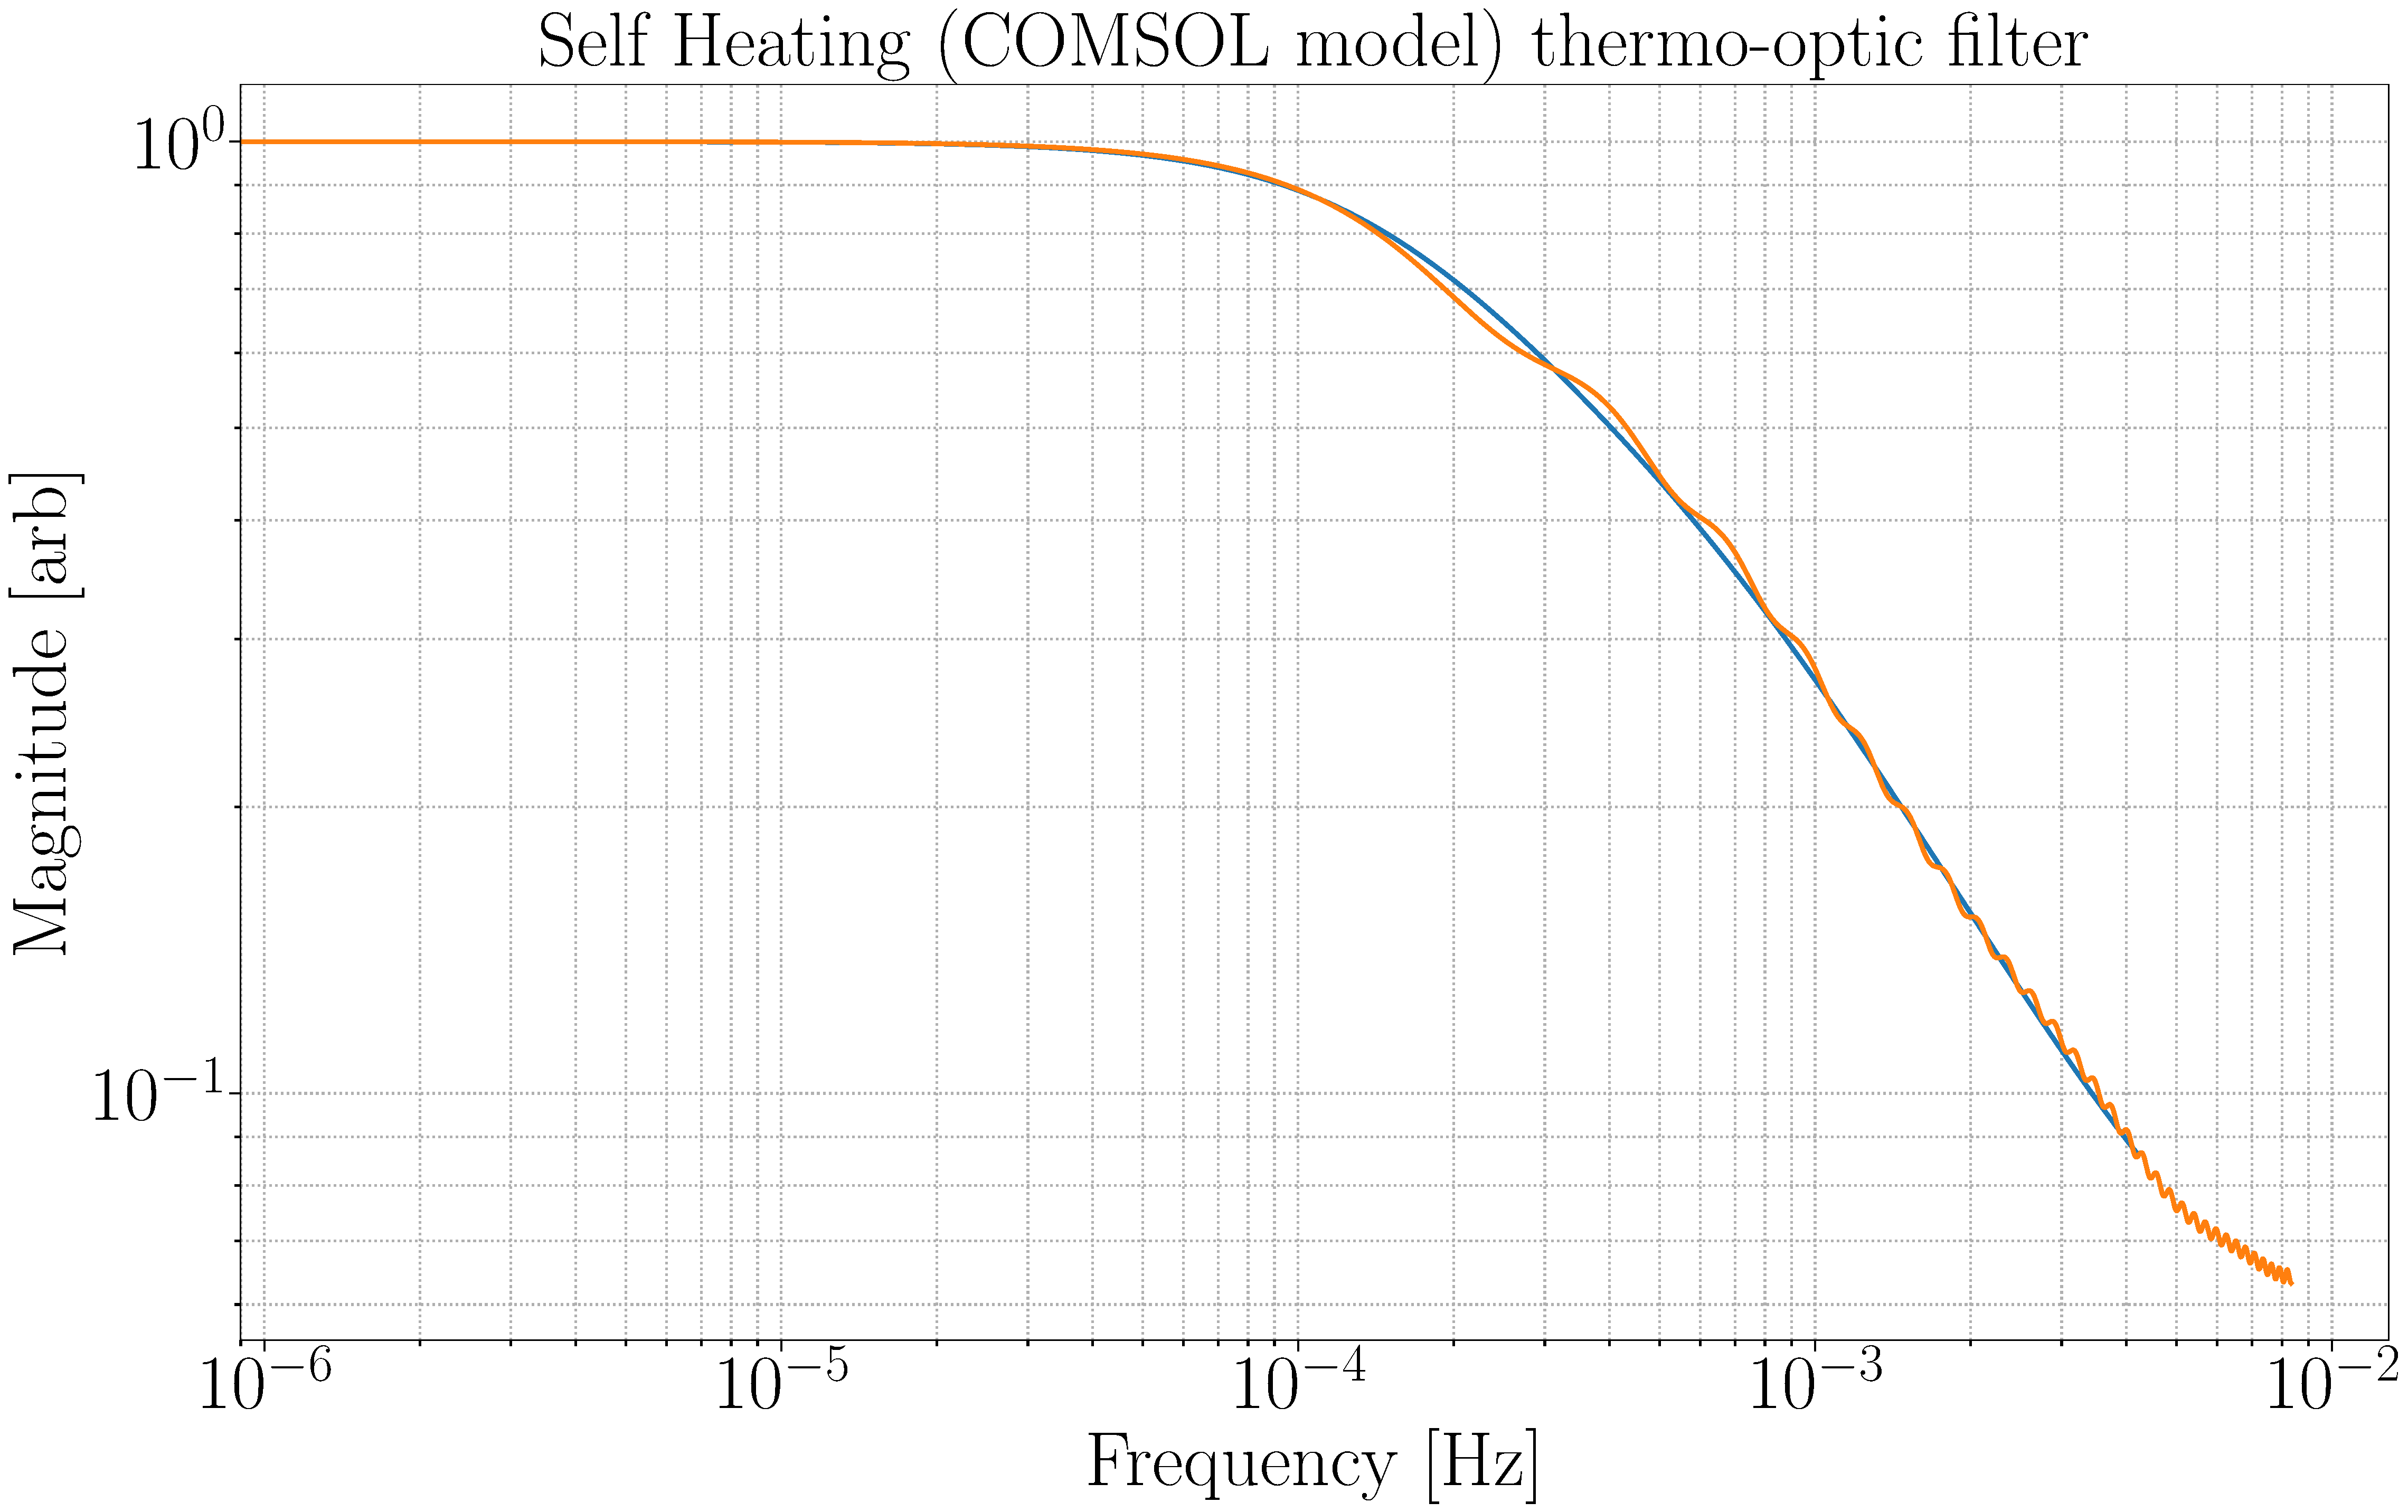
\includegraphics[width=\textwidth]{figs/TCS/self_heating_zpk.pdf}
\caption{Fitted zpk filter to transient response of self heating COMSOL model.}
\label{fig:self_zpk_fit}
\end{figure}

\subsection{CO2 filter}
\begin{figure}[H]
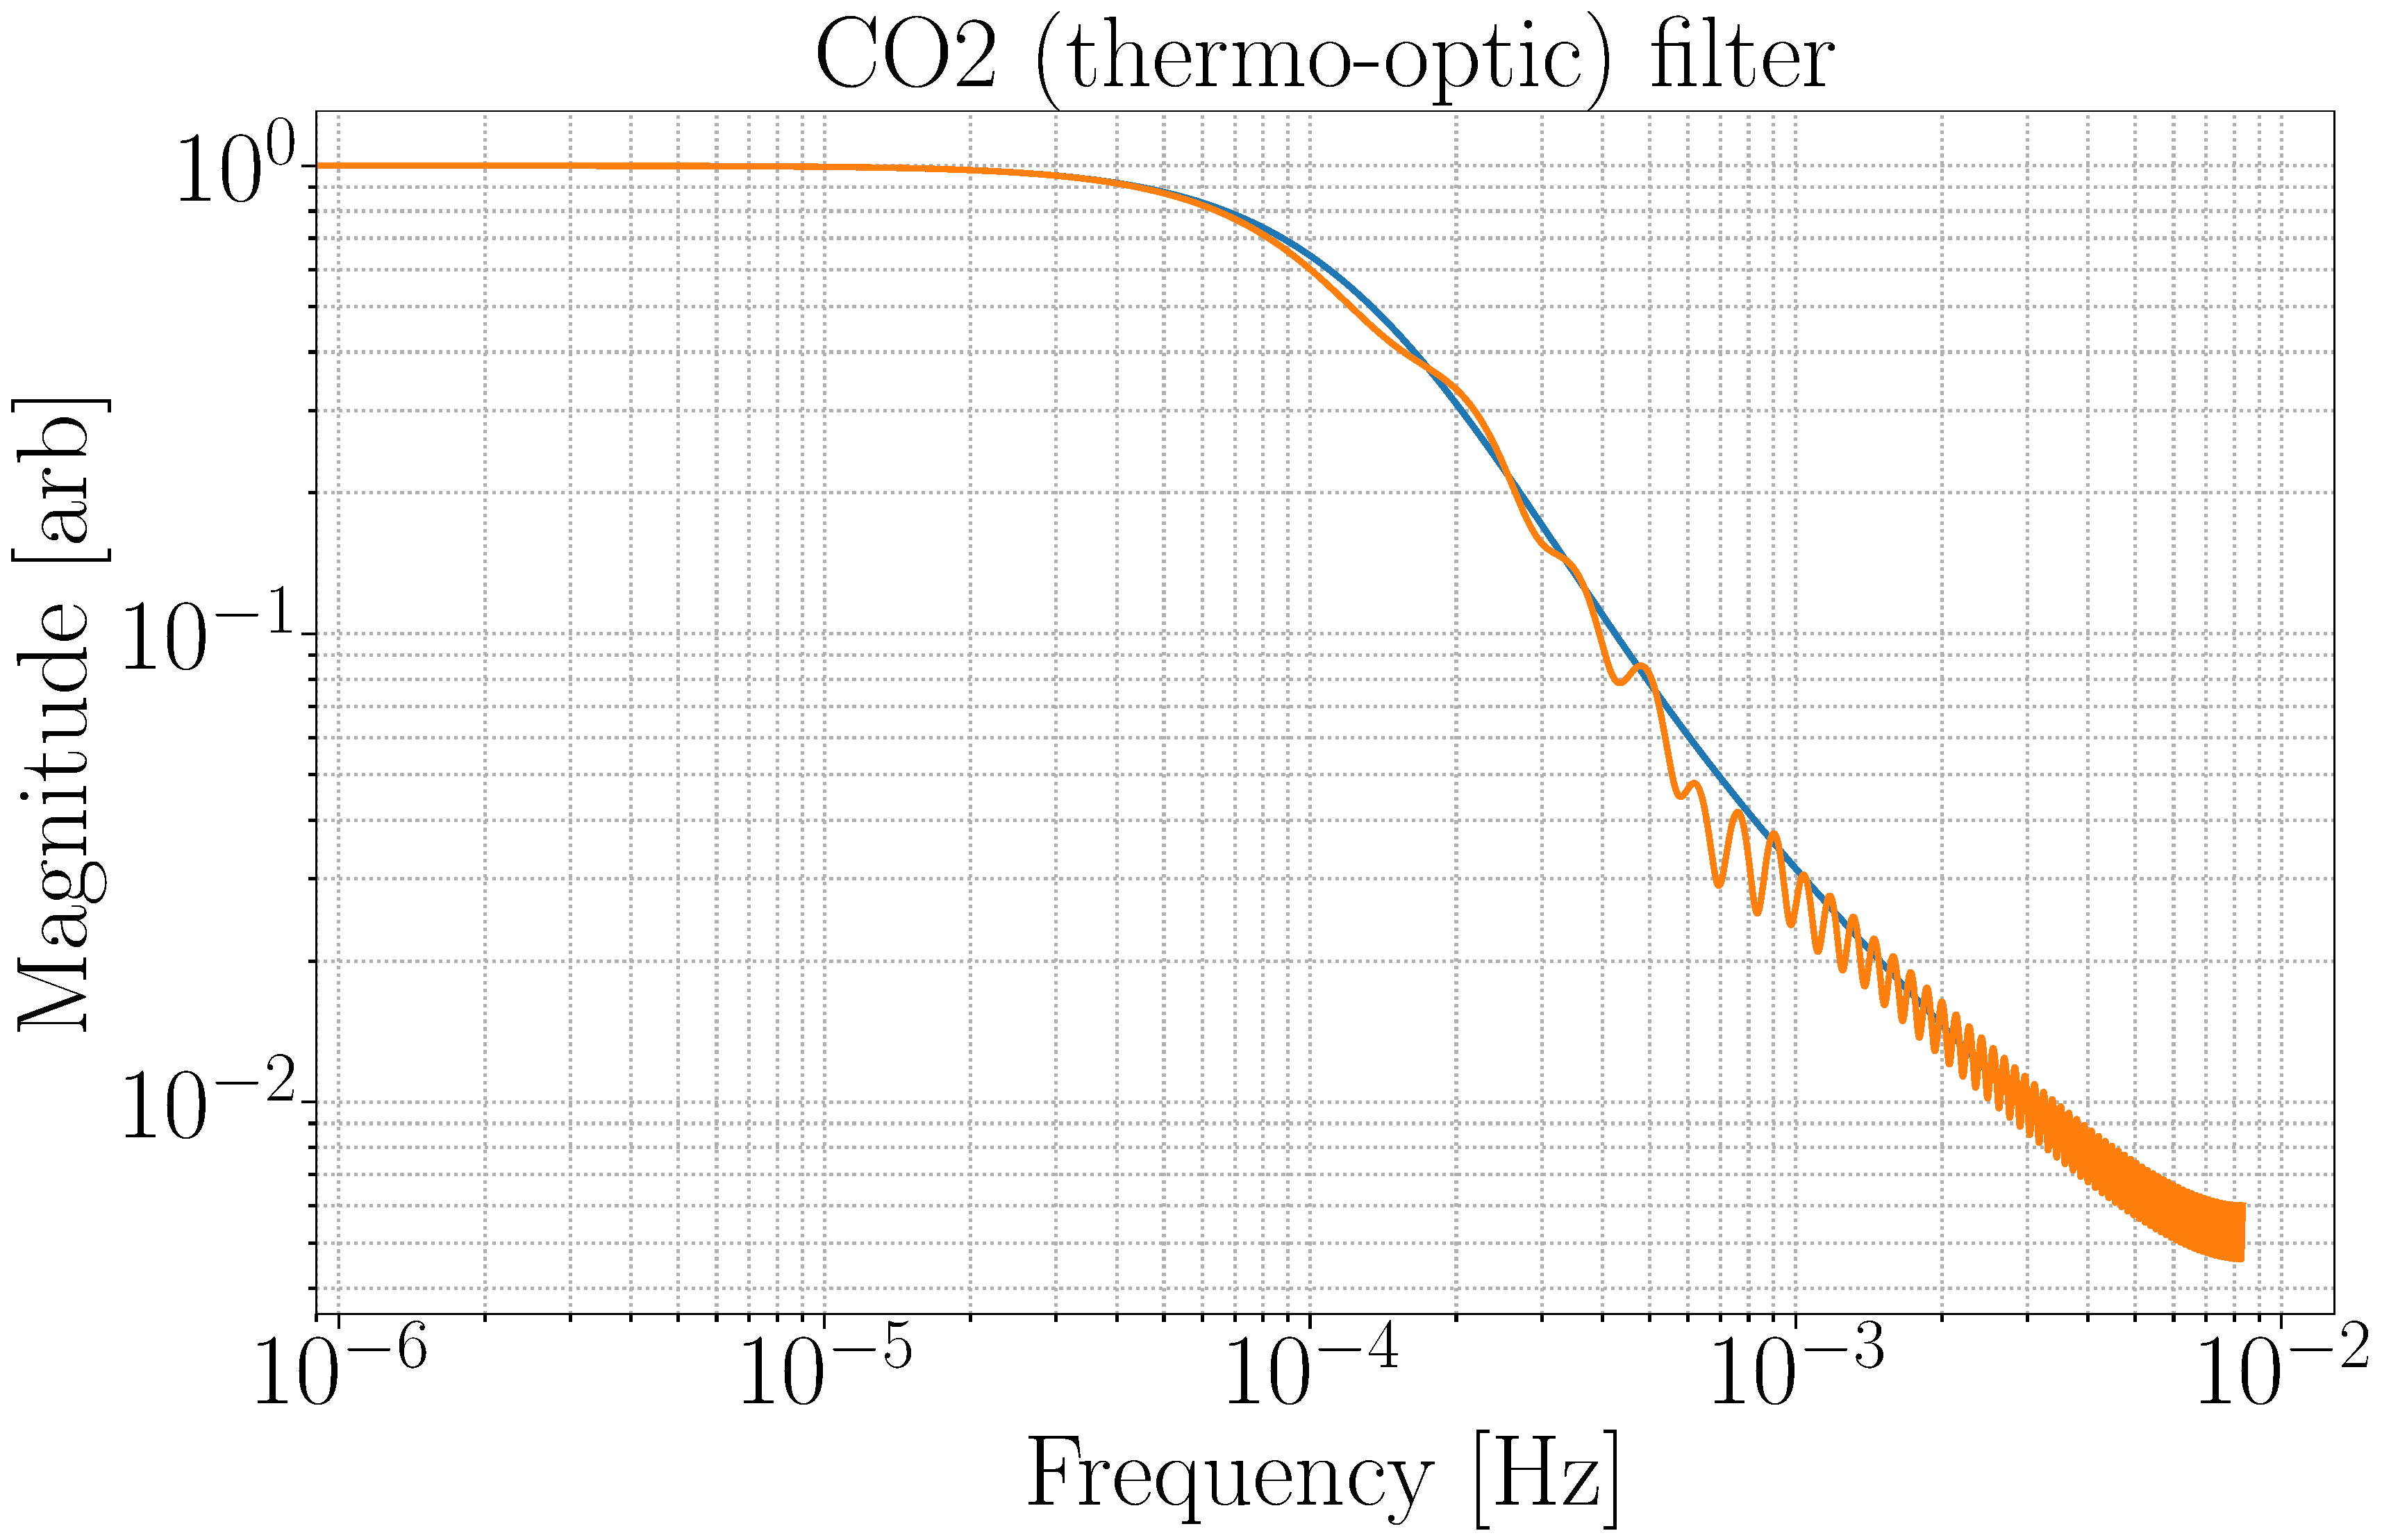
\includegraphics[width=\textwidth]{figs/TCS/CO2_zpk.pdf}
\caption{Fitted zpk filter to transient CO2 actuation response.}
\label{fig:co2_zpk_fit}
\end{figure}

\newpage
\section{Thermo-optic Path Distortion (analytical)}
\subsection{Thermorefractive aberration}
Consider an aberration of a substrate with an uninfluenced index of $n_0$ and a thermo-refractive term ($\frac{dn}{dT}$):
\begin{equation}
n(x,y,z) = n_0 + \frac{dn}{dT} [T(x,y,z) - T_0]
\end{equation}

The above coorelates the material index ($n$) to a path distortion ($\Psi$) (to first order) from thermal aberrations on a cylindrical substrate volume \cite{hellovinet:1990}:
\begin{equation}
    \Psi(r) = \frac{dn}{dt} \int^{h/2}_{-h/2} [T(r,z) - T_0] \;dz
\end{equation}

\subsection{Thermoelastic aberration}
A much more involved derivation with a significantly larger result than above is computed in \cite{hellovinet_te:1990}, though best computed for oneself especially for coatings and substrates alternative to $\siotao$ and fused silica respectively. It is worth mentioning that the effect for an approximate 1W absorbed power yields a 10 times smaller optical path distortion than that mentioned for the thermal lens~\cite{hellovinet:1990}. 

\subsection{Ring Heater actuation}
\begin{equation}
	\Psi(t,r)=2\frac{dn}{dT} \sum^{\infty}_{m,p = 1} A_{m,p} \; c^{u}_{p} \mathrm{sin}(u_m h /2a) (a/u_m)[1-e^{-\alpha t}] J_0(\zeta_p r/a)
\end{equation}
~\cite{ramette:2016}

\section{CO2 mask}\label{sec:CO2mask}
\begin{figure}[H]
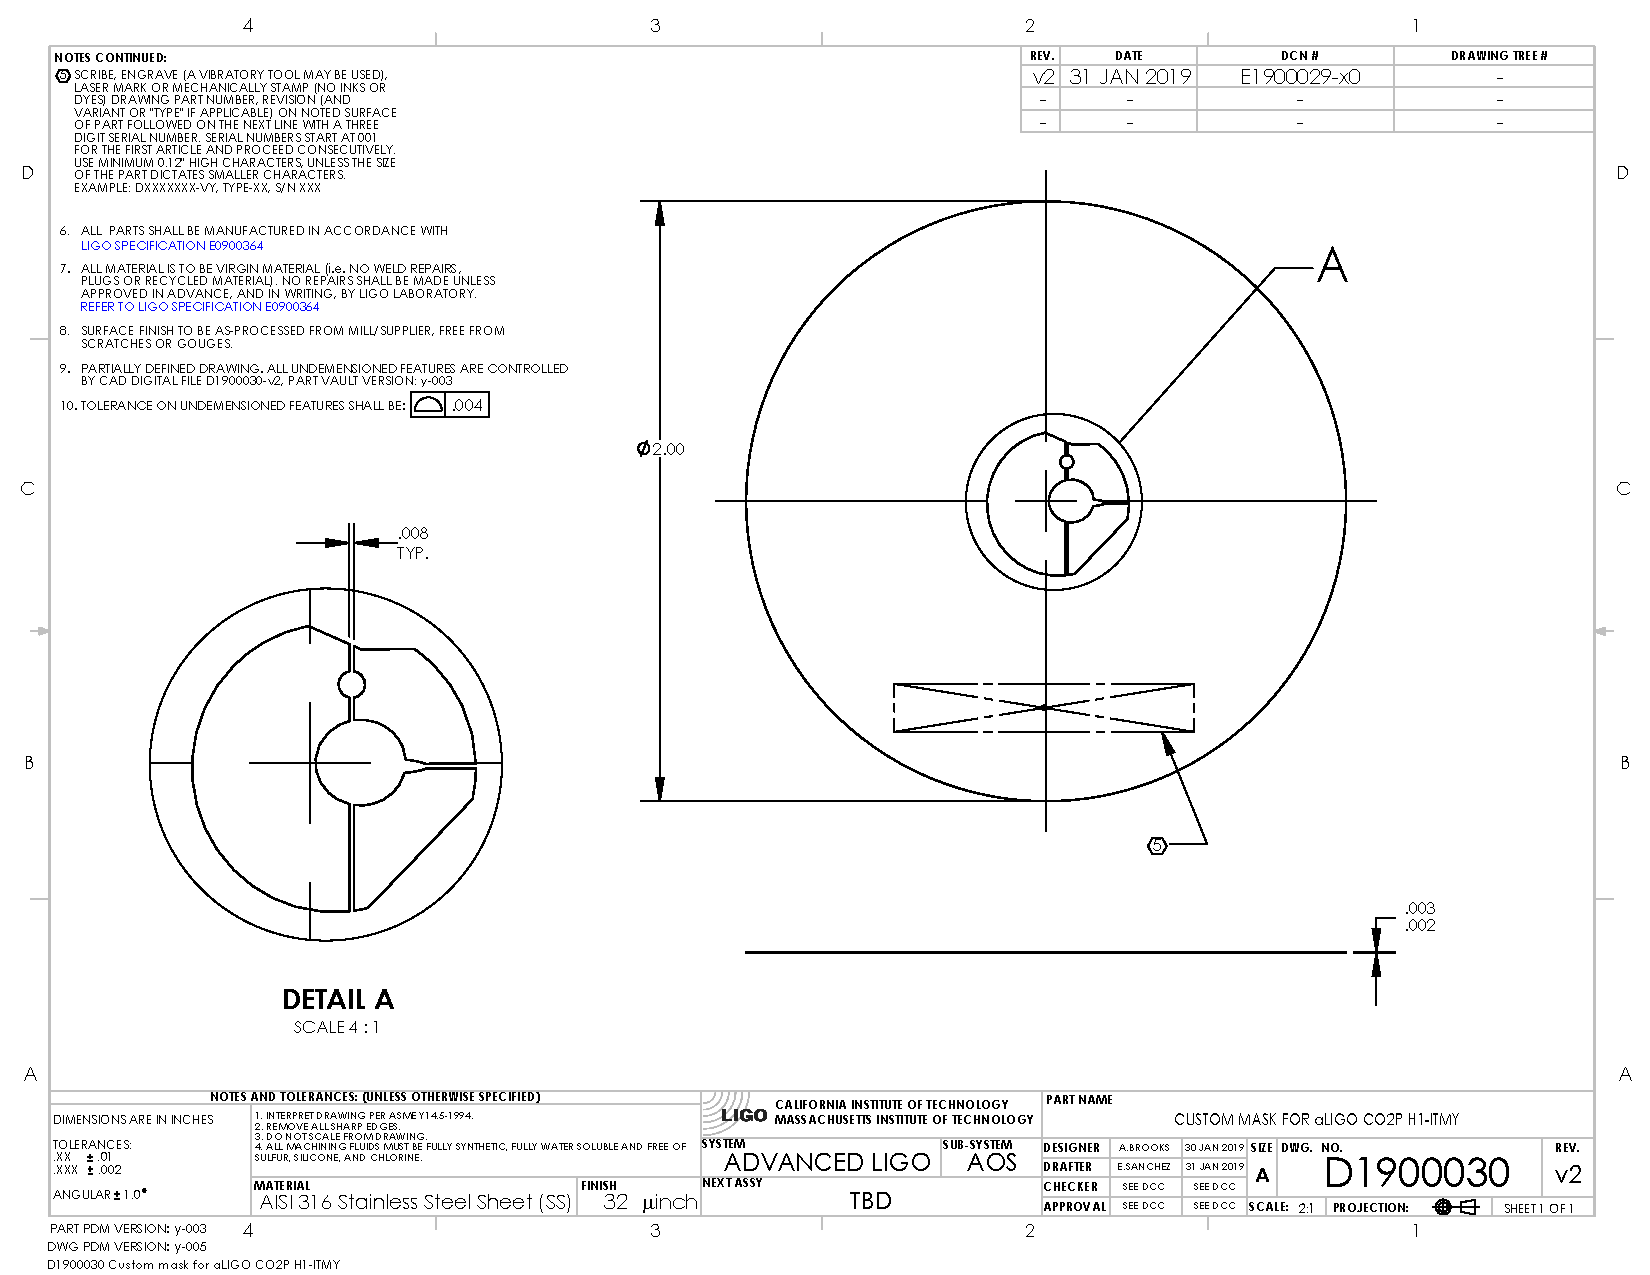
\includegraphics[width=\textwidth]{figs/TCS/CO2mask/D1900030-v2.PDF}
\caption{A CAD drawing of the first CO2 mask installed in the CO2 beam path.}
\label{fig:co2mask1}
\end{figure}

\newpage
\section{Anisotropic media}
Unlike isotropic media, we do not assume that the index of refraction of anisotropic media is the same for all chosen wave vectors. This is a direct consequence of the birefringence of anisotropic media; characterized by the dielectric, permittivity, and polarization tensors.

\subsection{Monochromatic plane wave propogation}
Revisiting Maxwell's equations for a simple monochromatic plane wave solution provides further direction on how crystalline media may effect incident light. Further elaborating, the following assumptions are made:
\begin{equation}
\vec{E} = E_o e^{(i \omega (\frac{n}{c} \vec{r}\cdot \vec{s}-t))}
\end{equation}
Where $n$ is the index of refraction, $c$ is the speed of light, $\vec{r}$ is the position vector and $\vec{s}$ is the unit wave normal.
\begin{equation}
\nabla \times \vec{H}= \frac{\partial \vec{D}}{\partial t}
\end{equation}
Where $\vec{H}$ is the magnetic field assuming permeability $\mu$, and the generalized displacement vector $\vec{D}$ and electric field vector $\vec{E}$.
\begin{equation}
\nabla \times \vec{E} = -\mu \vec{H}
\end{equation}
Reducing to only the displacement and electric fields:
\begin{equation}\label{eq:dispelec}
\vec{D} = \frac{n^2}{\mu}[\vec{E}-\vec{s}(\vec{s}\cdot \vec{E})]
\end{equation}
Maxwell's equations show that the electric field is not necessarily parallel to the displacement field and in most materials with non-zero polarizability tensors and dielectric tensors, it is not. But as specified above, the displacement vector, Electric field and unit wave normal are co-planar while remaining orthogonal to $\vec{H}$. Assuming we are operating within a coordinate system aligned with the principal dielectric axes, we substitute \autoref{eq:dispfield} into \autoref{eq:dispelec}:
\begin{equation}
E_i = \frac{n^2 s_i (\vec{E}\cdot\vec{s})}{n^2 - \mu \varepsilon_i}
\end{equation}

From here it can be shown that for a general plane wave there exist two unique refractive index solutions within the constructed dielectric ~\cite{nye}. 

\subsection{The Dielectric tensor} \label{appendix:Diel_tensor}
Further elaborating on the nature of a generalized dielectric tensor ($\varepsilon$) for any wavevector is required to proceed:
\begin{equation}\label{eq:dispfield}
D_i = \varepsilon_{ij}E_j
\end{equation}
Where D is the displacement vector, E is the electric field vector, and $\varepsilon$ is the dielectric tensor. The displacement vector for isotropic media is retrieved when $i = j$ and $\varepsilon_i = \varepsilon$. To further understand the nature of the dielectric tensor we assert Poynting's theorem providing an energy conservation requirement:
\begin{equation}\label{eq:poynting}
\nabla \cdot \vec{S} = \frac{dU}{dt}
\end{equation}
Where $\vec{S} = \vec{E} \times \vec{H}$ is the poynting vector and $U = \frac{1}{8 \pi} \big( \vec{E} \cdot \vec{D} + \vec{B} \cdot \vec{H} \big)$ is the electromagnetic field density. The reader is left to perform the exercise and show that in order for \autoref{eq:poynting} to hold true given \autoref{eq:dispfield}


\begin{equation}
\varepsilon_{ij} = \varepsilon_{ji}
\end{equation}
Demonstrating that the dielectric tensor is symmetric - exhibiting only six unique terms. Diagonalizing the tensor, the presence of two unique eigenvectors and eigenvalues indicates the existence of two eigenpolarizations with paired eigenindices.

\begin{equation}\label{eq:modelec}
E_i = \frac{n^2 s_i (\vec{E}\cdot\vec{s})}{n^2 - \mu \varepsilon_i}
\end{equation}

Though this result requires revisiting geometrical conditions that are best visualized using a method introduced in the next section \cite{nye}. 

%The most general form of the energy density can be geometrically represented as ellipsoid but a coordinate transformation we can diagonalize and realize the principal axes of the dielectric allowing a simpler form of the displacement, and in turn the energy density.

\section{Miller indices for highly reflective $\gaas$/$\algaas$ coatings}
\begin{figure}[!hb]
    \begin{subcaptiongroup}
	    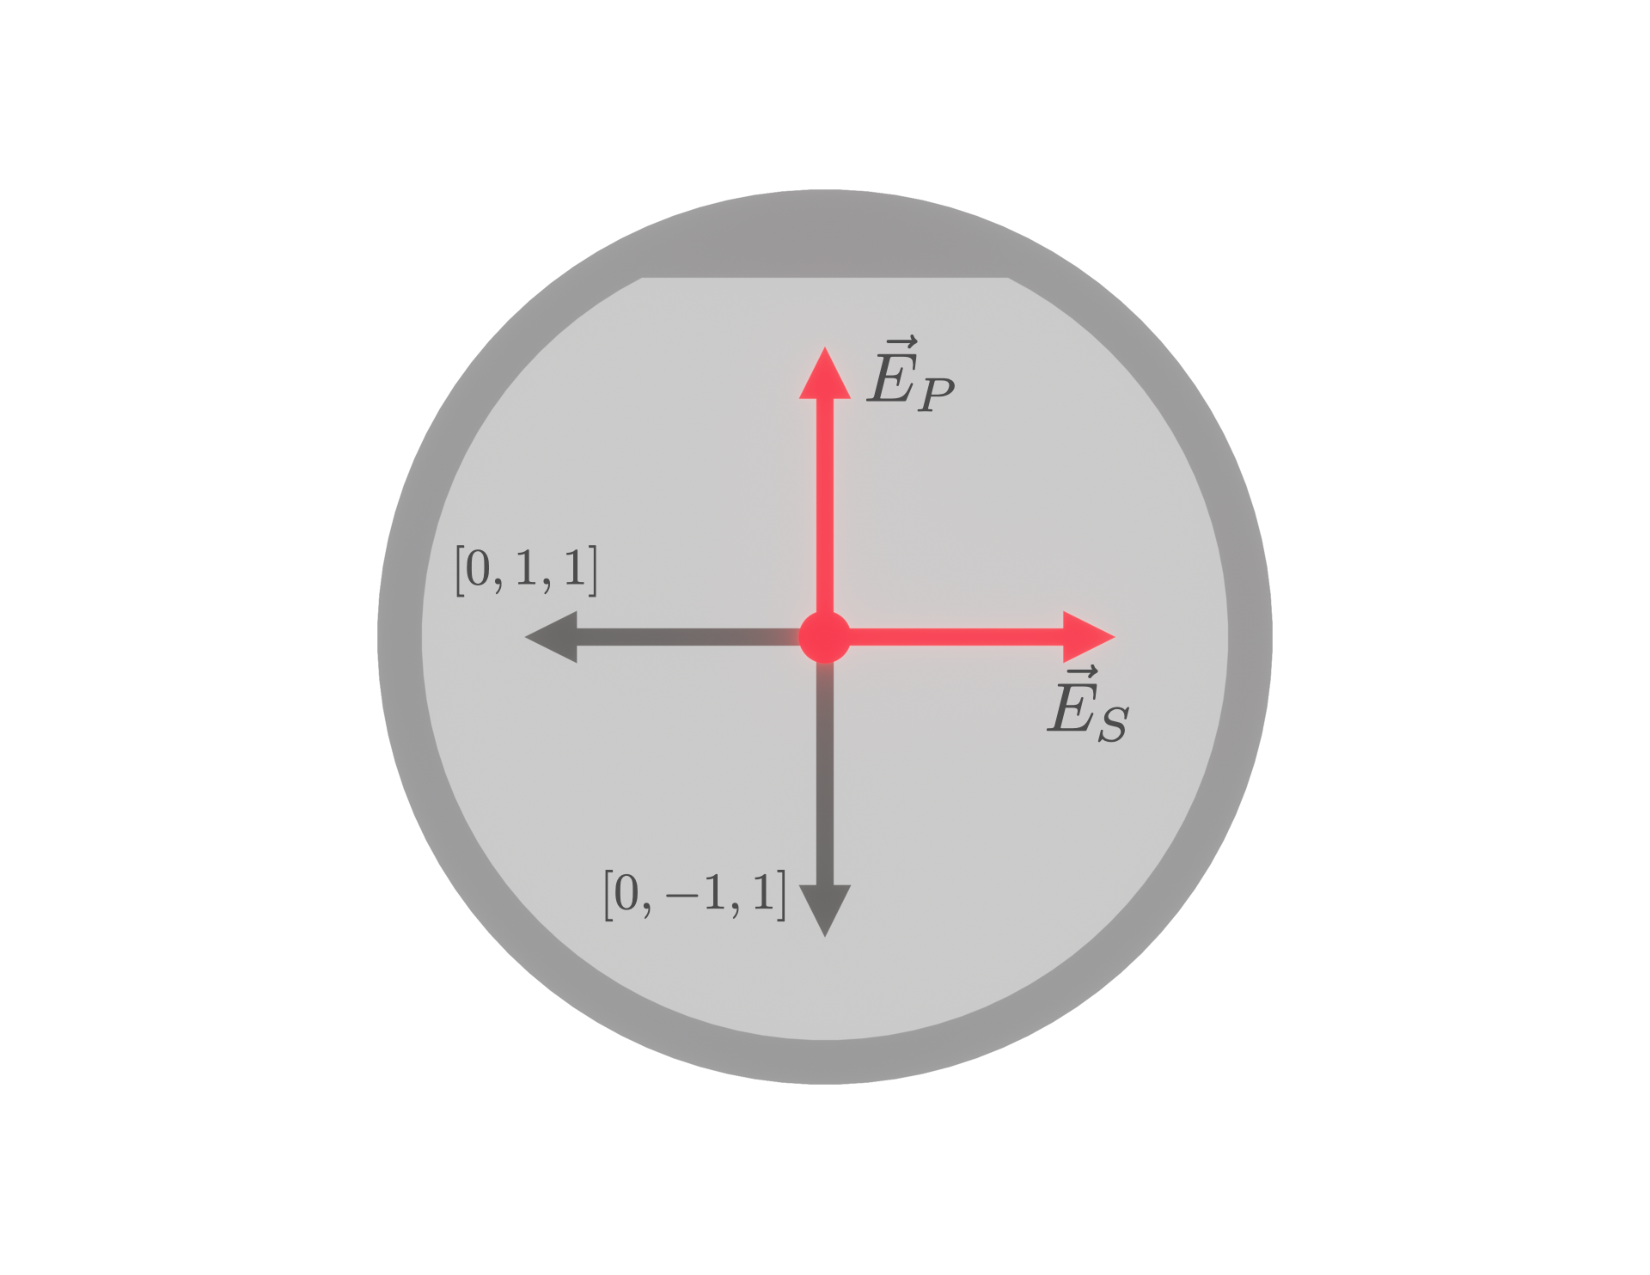
\includegraphics[width=.5\textwidth]{figs/ALGAAS/coating_orientation_normal.pdf}
	    \phantomcaption\label{conormal}
	    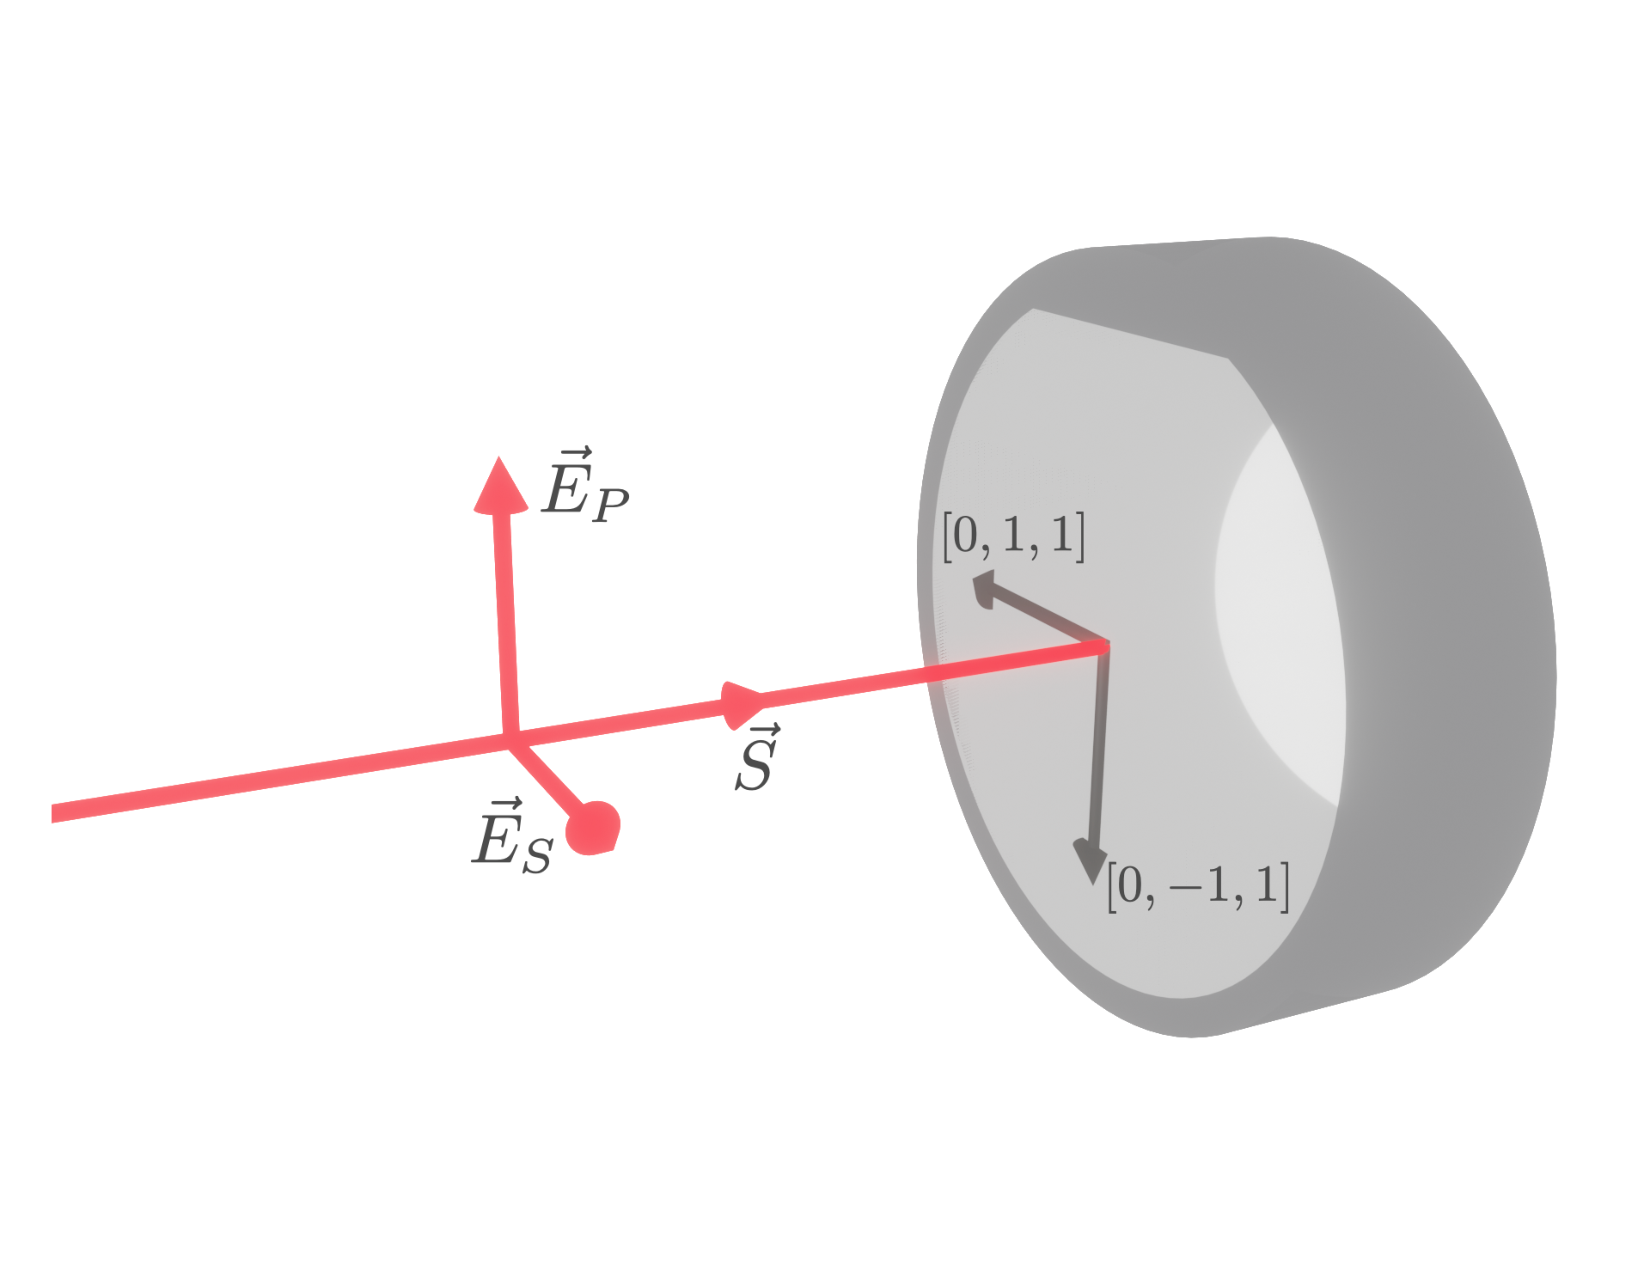
\includegraphics[width=.5\textwidth]{figs/ALGAAS/coating_orientation_isometric.pdf}
	    \phantomcaption\label{coiso}
    \end{subcaptiongroup}
\caption{The beam propogation axis ($\vec{S}$, $[-100]$) with respect to the $\gaas$/$\algaas$ crystal axes. The axis formed by the [100] plane normal is drawn parallel with the beam axis (z-axis) and the polarizations of incident and reflected beam oscillate along vectors within the plane formed by the normal of that axis. The coating is grown with a flat tracing a line within the [0-11] plane; where the plane normal points towards the sample center.}
\label{fig:algaascoords}
\end{figure}

Up to this point three varieties of orthonormal coordinates are addressed: the crystal axis (as indicated by Miller index plane normals), the principal dielectric axis (based on diagonalization of the indicatrix), and an optical beam axis (when considering a desired (laser) light propogation). The asserted beam axis can be cited \autoref{fig:algaascoords}.



\section{Mode matching data for Electro-optic sample cavity}

\subsection{Pre MMT beam scan}

\begin{figure}[H]
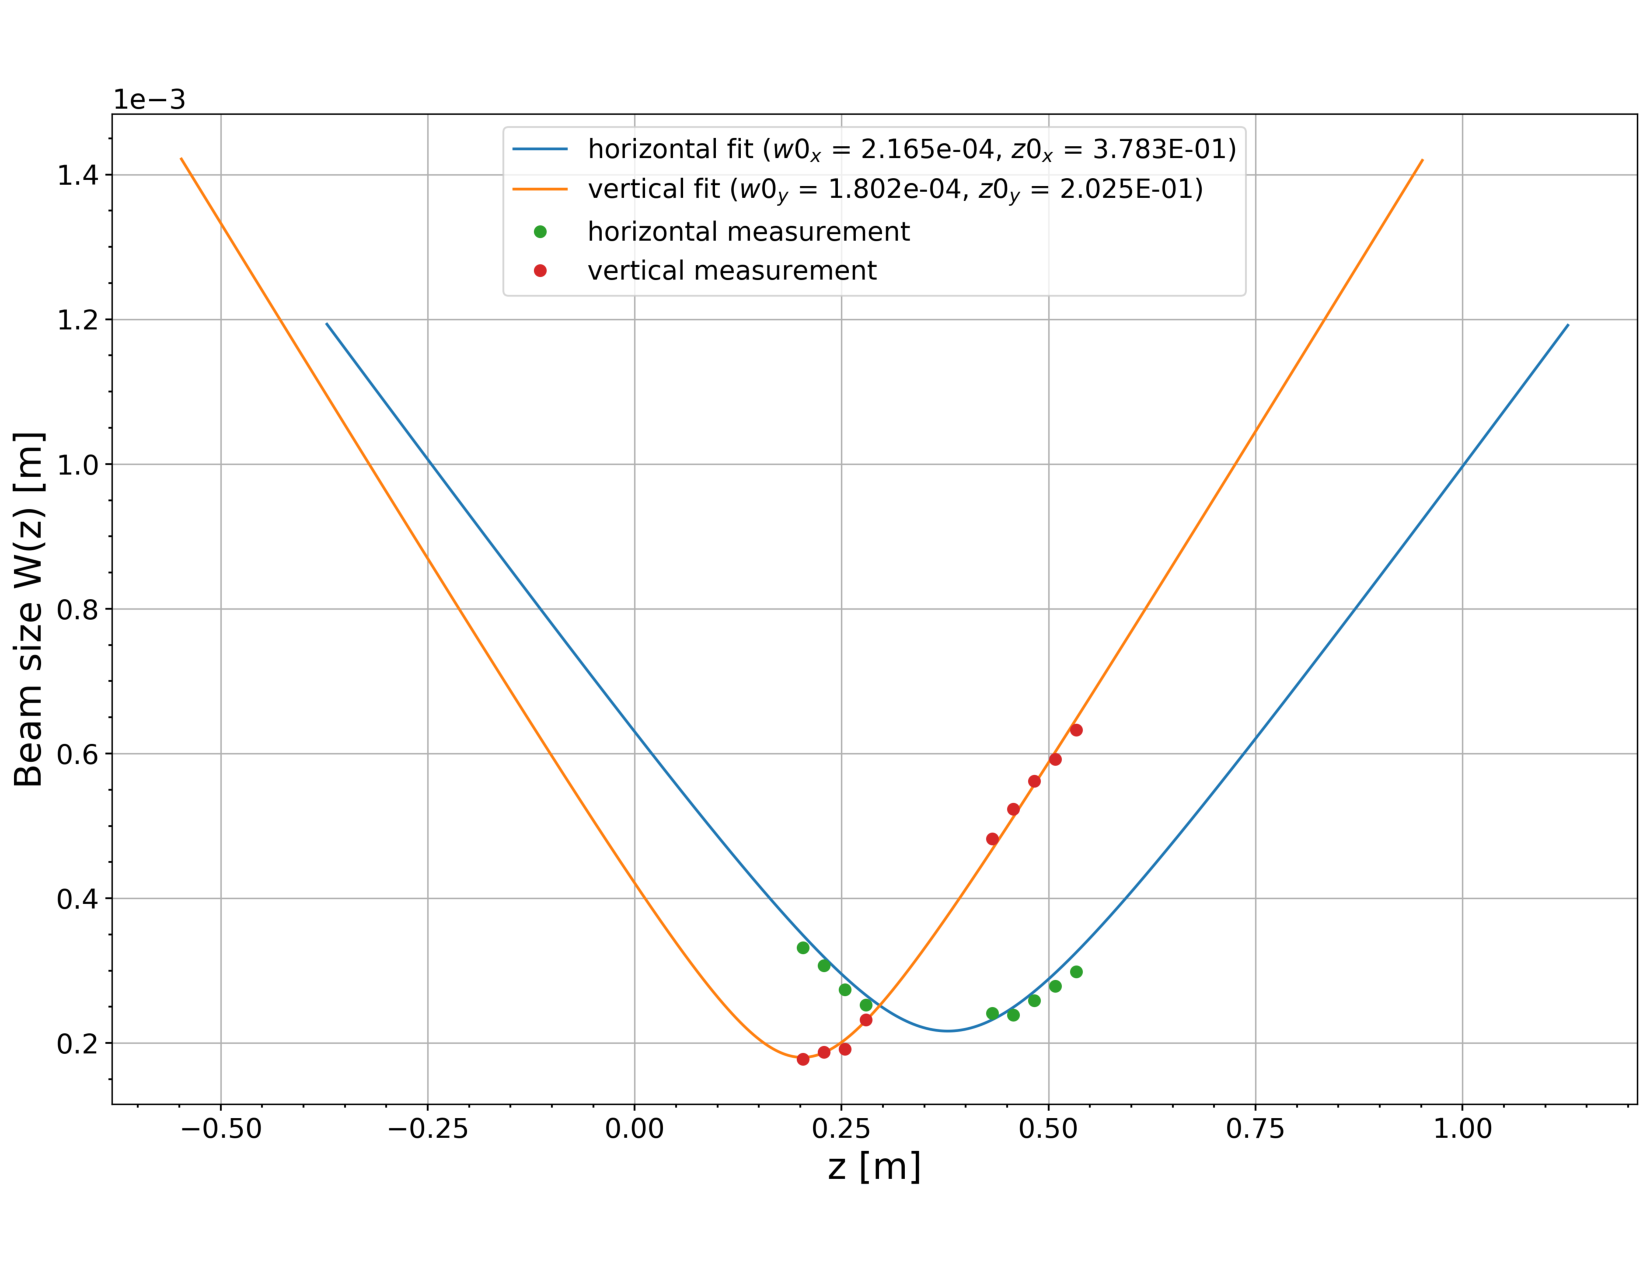
\includegraphics[width=.95\textwidth]{figs/ALGAAS/beam_scans/12_18_2020_preMMT.pdf}
\caption{Beam scan taken from SM5 (Steering mirror 5)}
\label{fig:beamscan2020}
\end{figure}

\subsection{``Just another mode matching tool" (JAMMT) solution}
\subsection{Post MMT beam scan}

\begin{figure}[H]
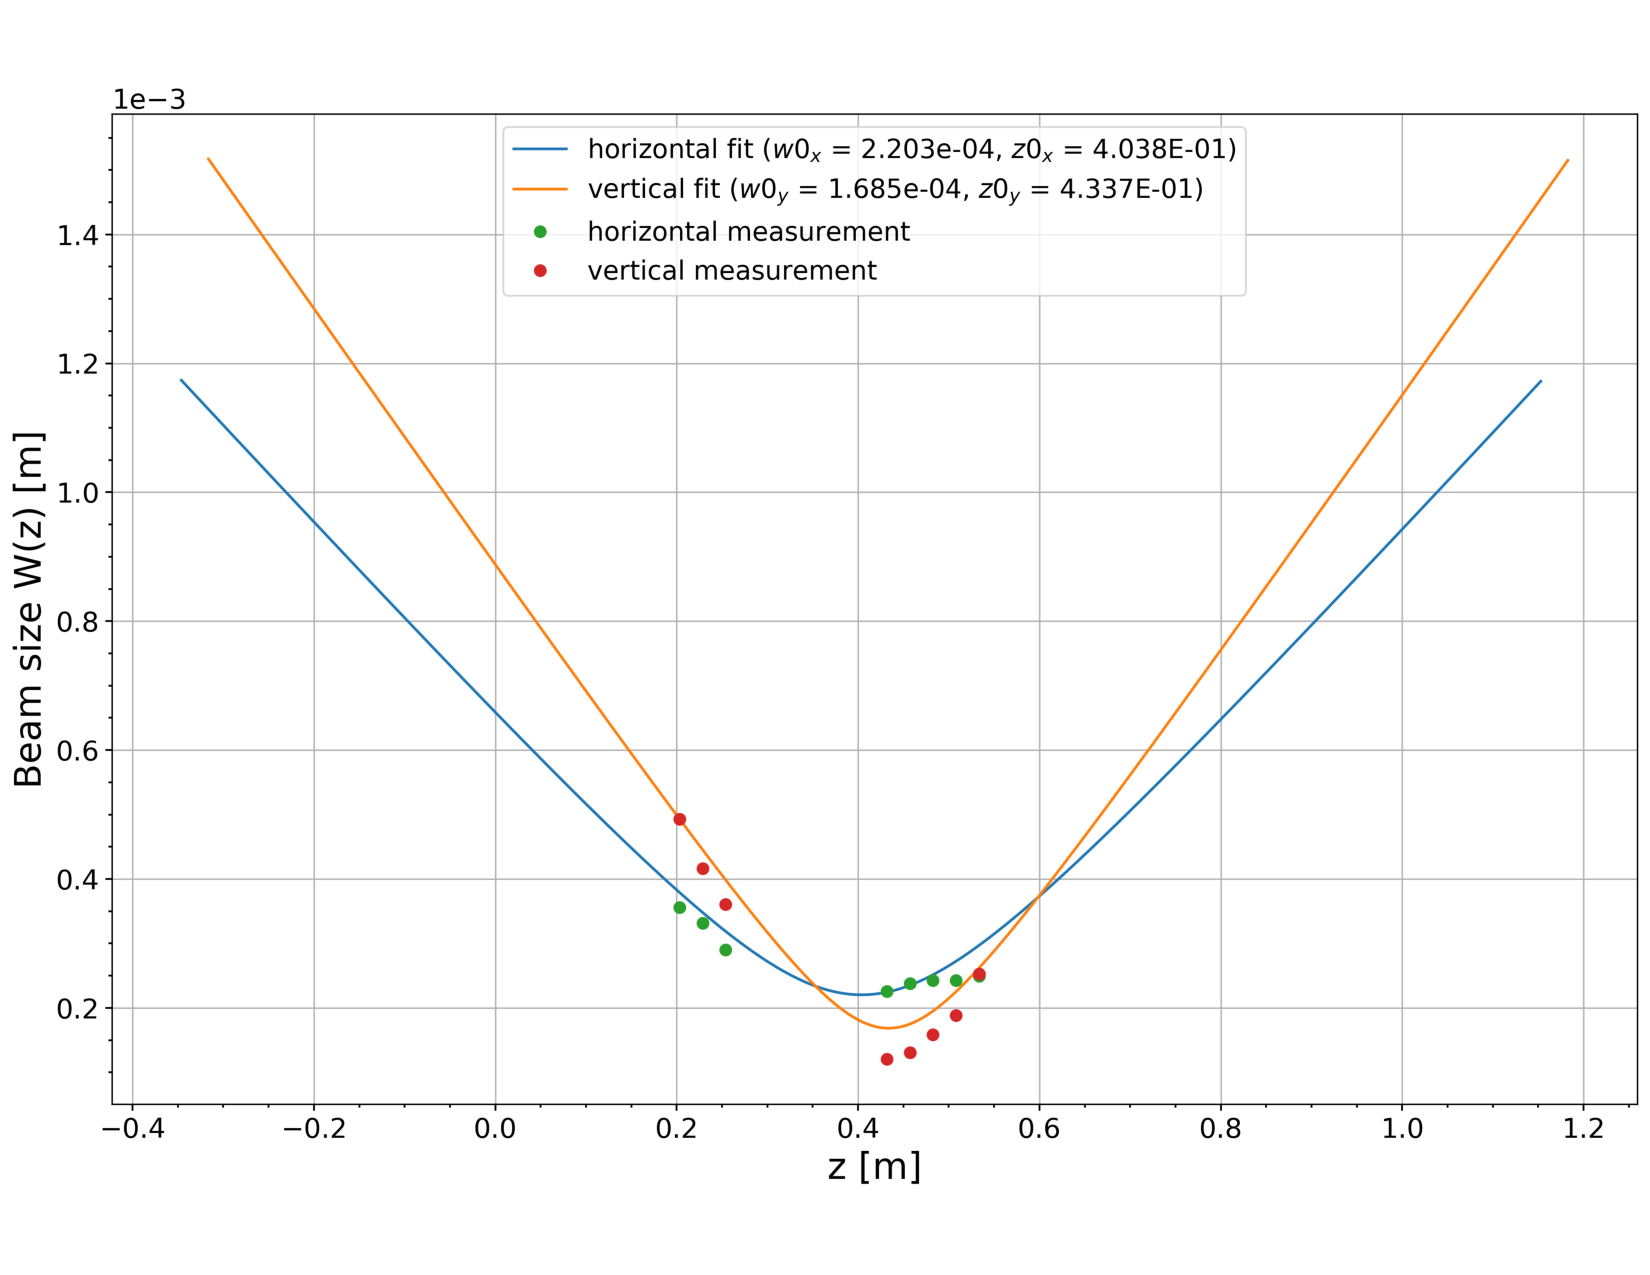
\includegraphics[width=.95\textwidth]{figs/ALGAAS/beam_scans/01_12_2021_postMMT.pdf}
\caption{Beam scan taken from SM6. Sampling points before SM7 and after the first cavity iris.}
\label{fig:beamscan2021}
\end{figure}

\section{Laser PZT sweep}\label{appendix:laser_sweep}

\begin{figure}[H]
	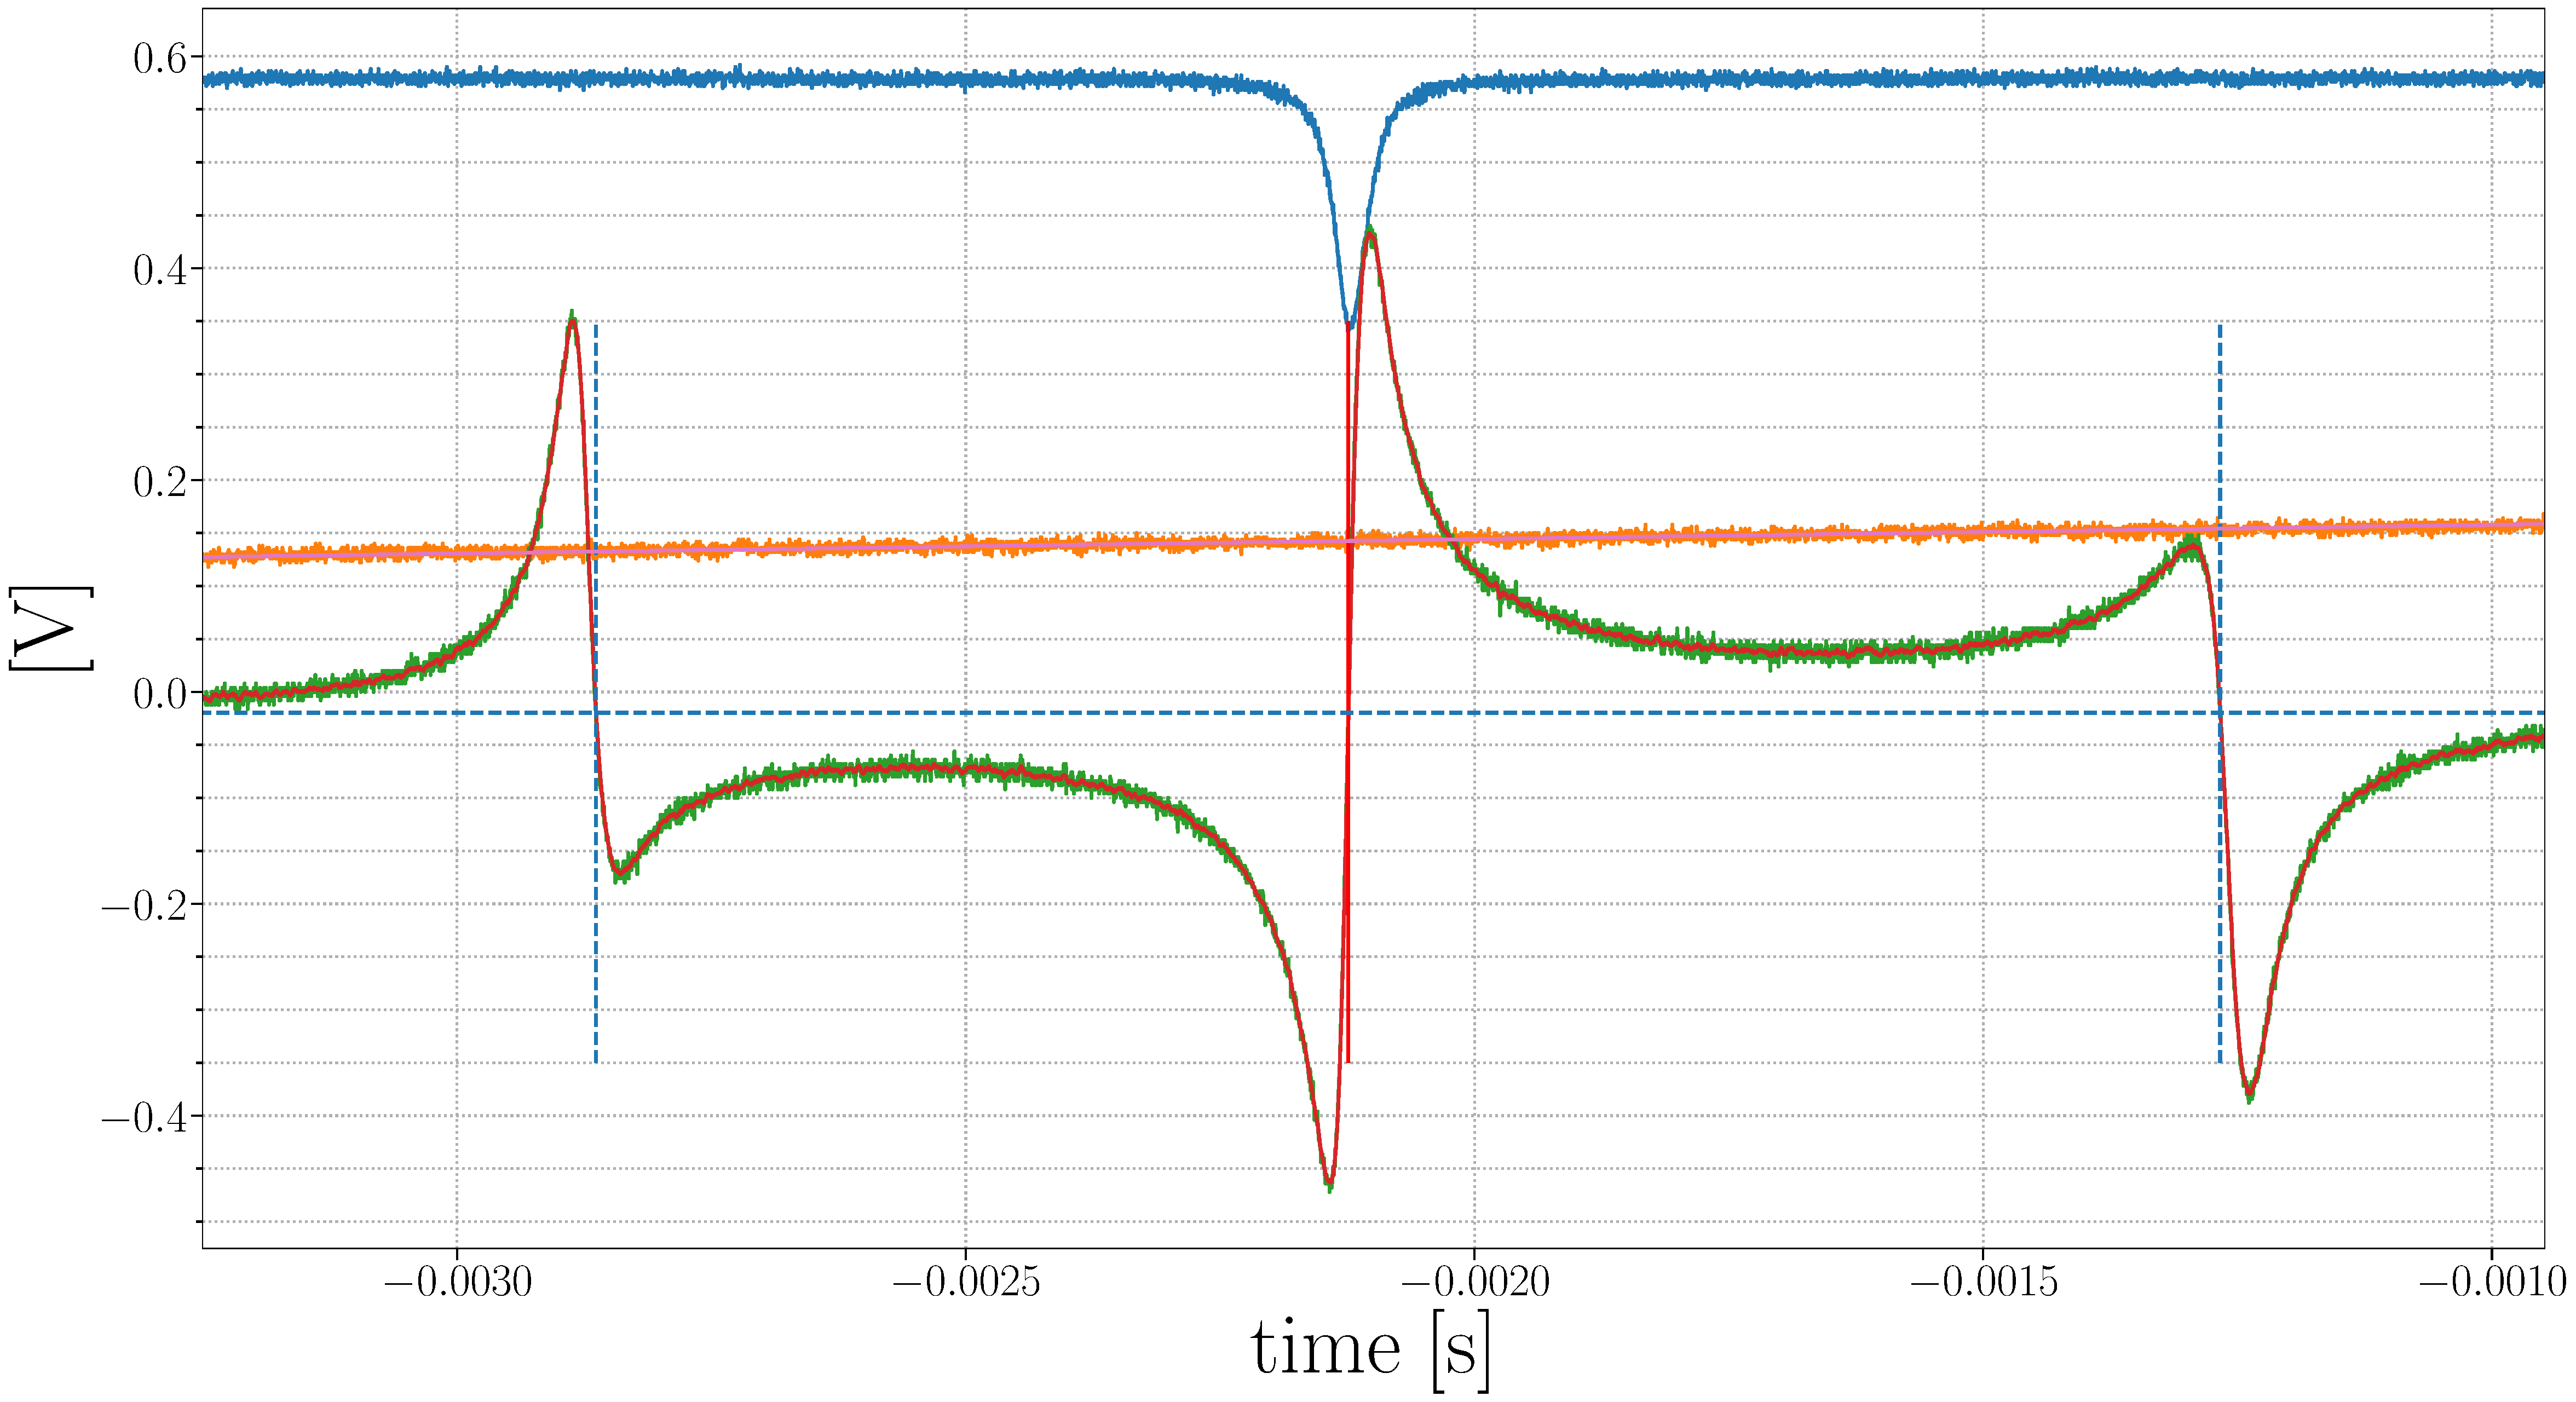
\includegraphics[width=.95\textwidth]{figs/ALGAAS/pdh_measured.pdf}
	\caption{Ramping voltage sent to the laser PZT while probing the mixer output. The sweep was performed for sample cavity of length notes}
\label{fig:pdhmeasured}
\end{figure}

\section{High Voltage Amplifier (HVA) transfer functions [V$_\mathrm{out}$ / V$_\mathrm{in}$]}\label{appendix:hva_tfs}
\begin{figure}[H]
    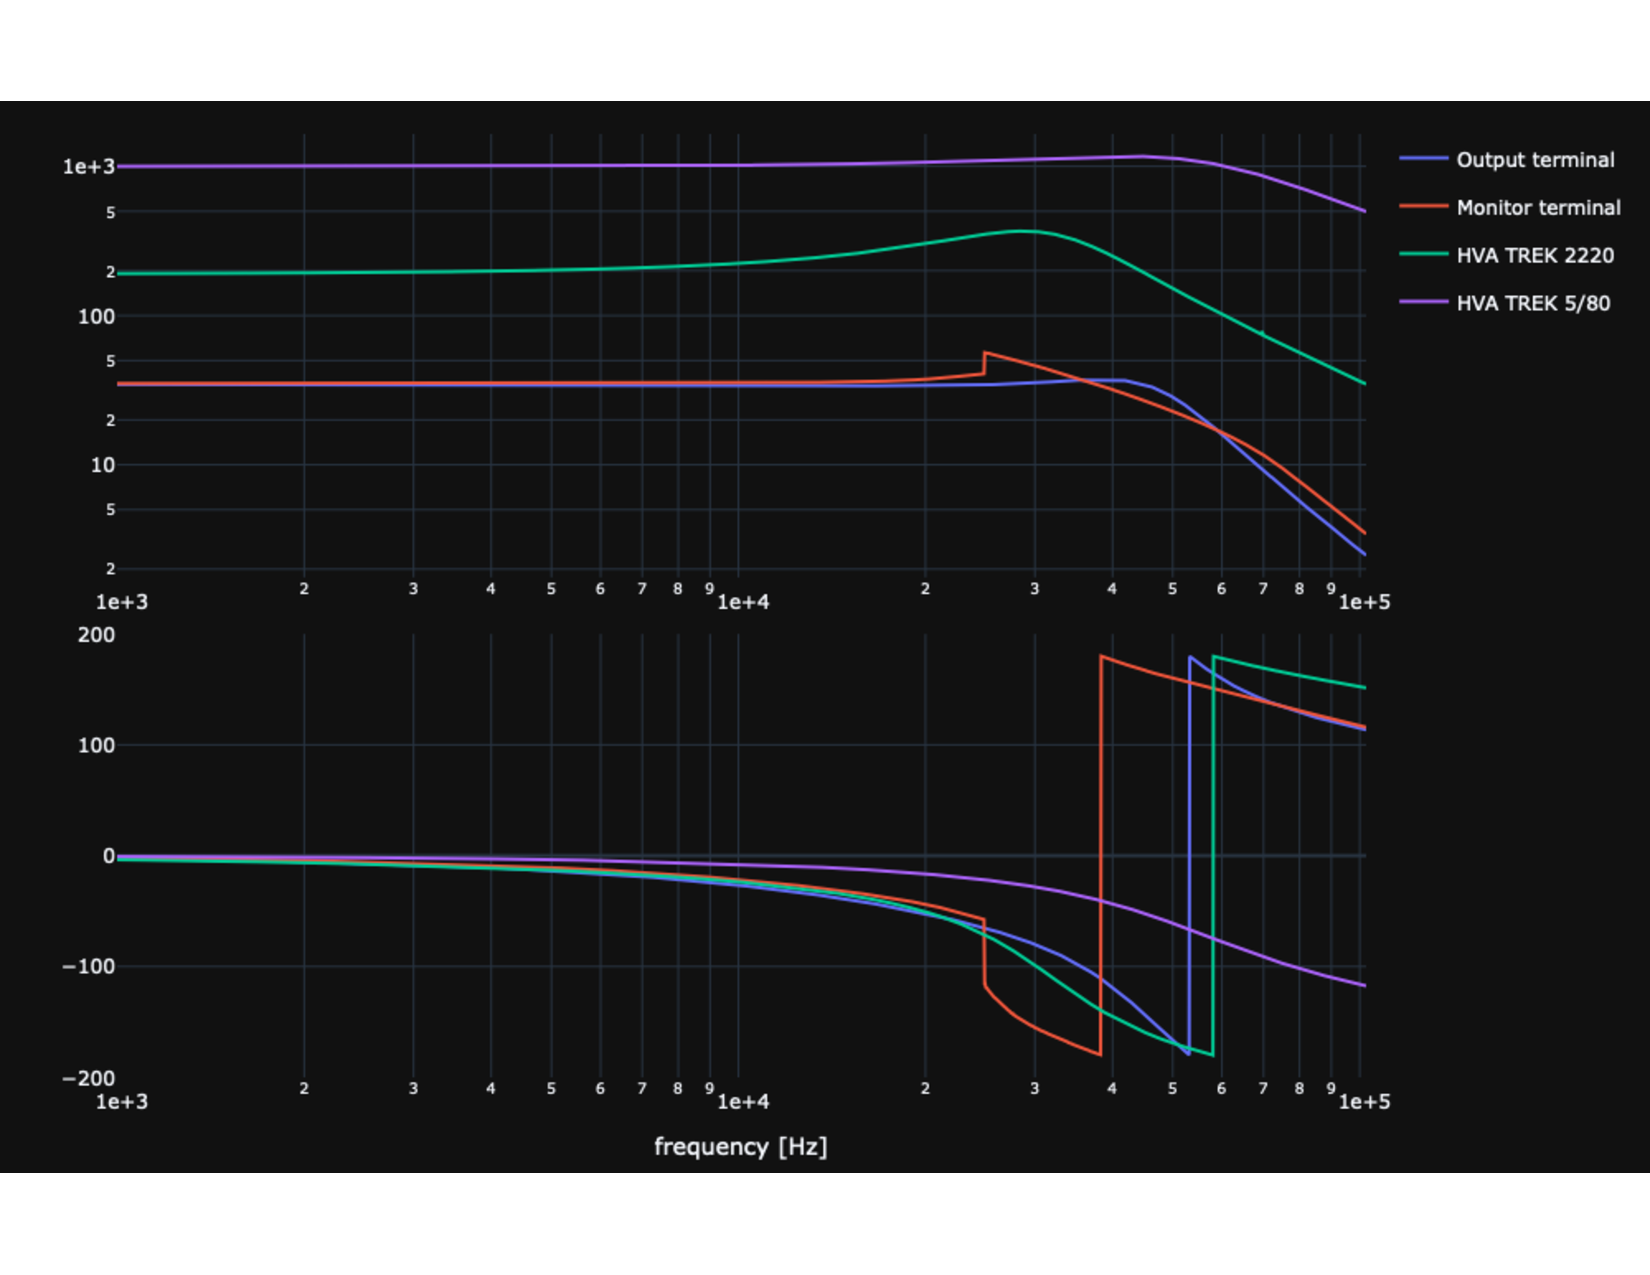
\includegraphics[width=\textwidth]{ALGAAS/tfs/hva_compare.pdf}
    \caption{Different high voltage amplifier transfer functions used for the study}
    \label{fig:hvacompare}
\end{figure}

\begin{landscape}
    \section{FSS transfer function (LTSPICE)}\label{appendix:fss_tf}
\begin{figure}[H]
  \begin{center}
    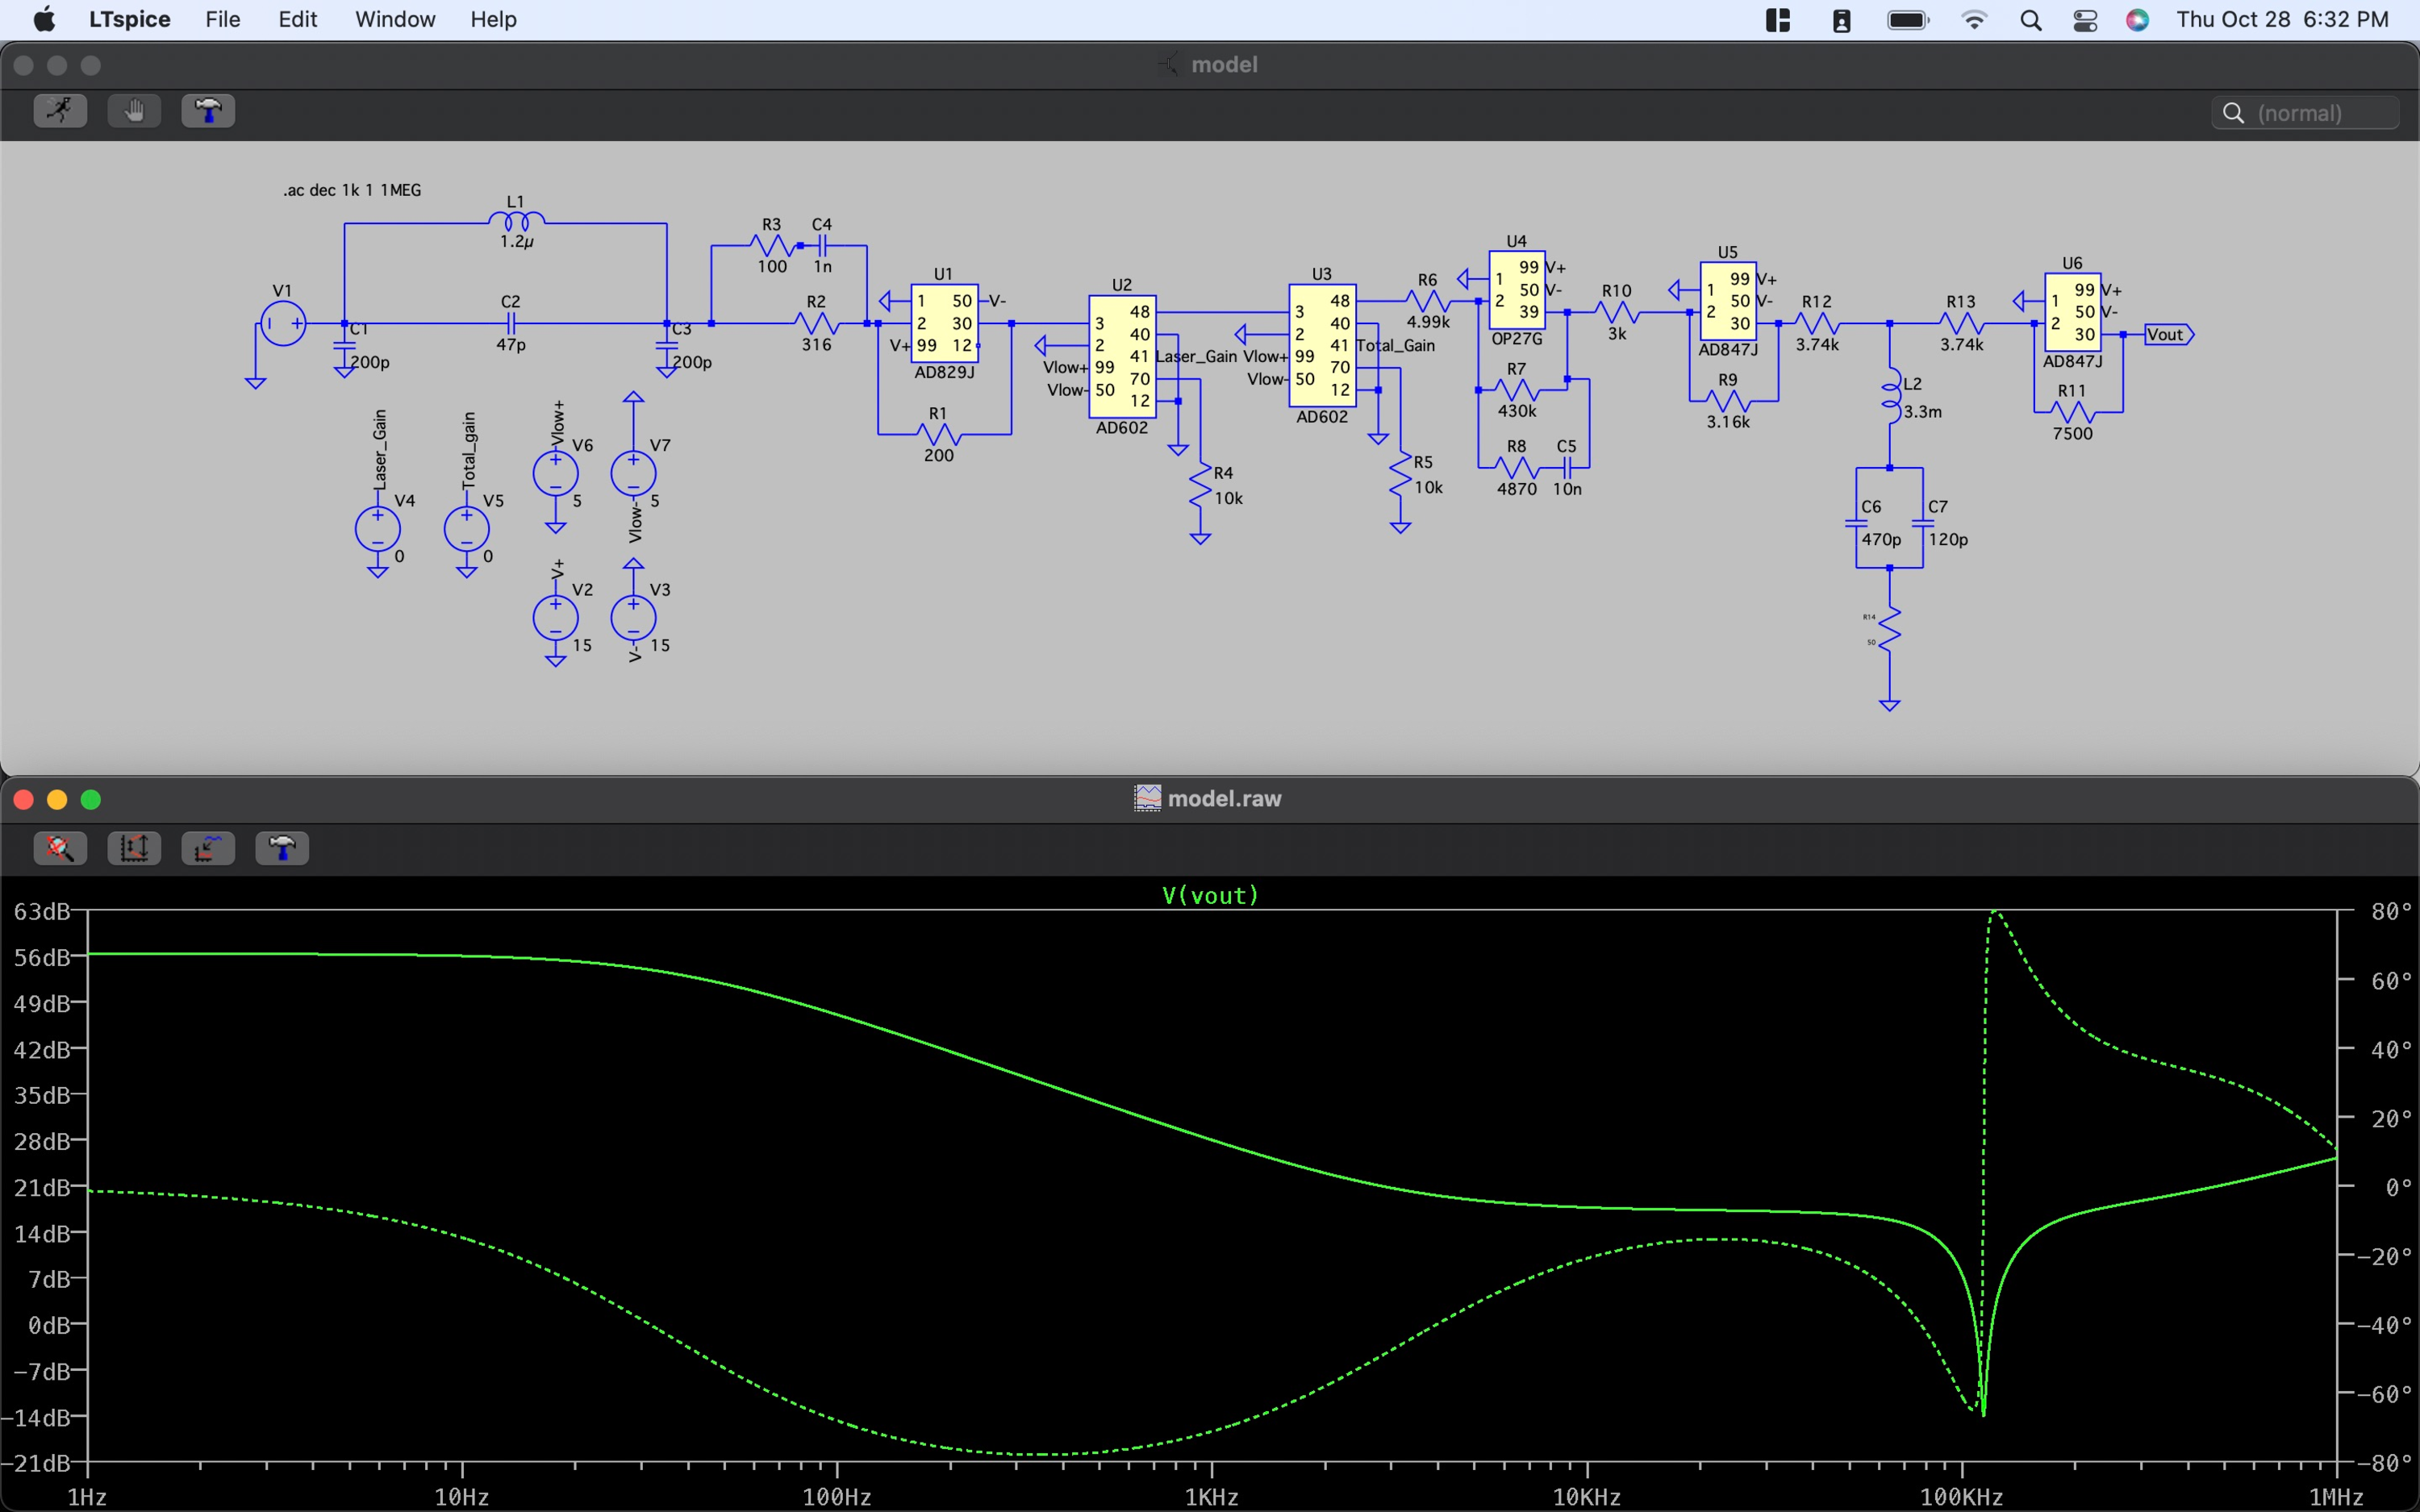
\includegraphics[width=1.33\textwidth]{figs/ALGAAS/tfs/spice_FSS_tf.pdf}
    \caption{The FSS frequency response simulated in LTspice}
  \end{center}
  \label{fig:spiceFSS}
\end{figure}
\end{landscape}

\section{Measuring OLG [H]}\label{appendix:OLG_meas}

\begin{figure}[H]
  \begin{center}
    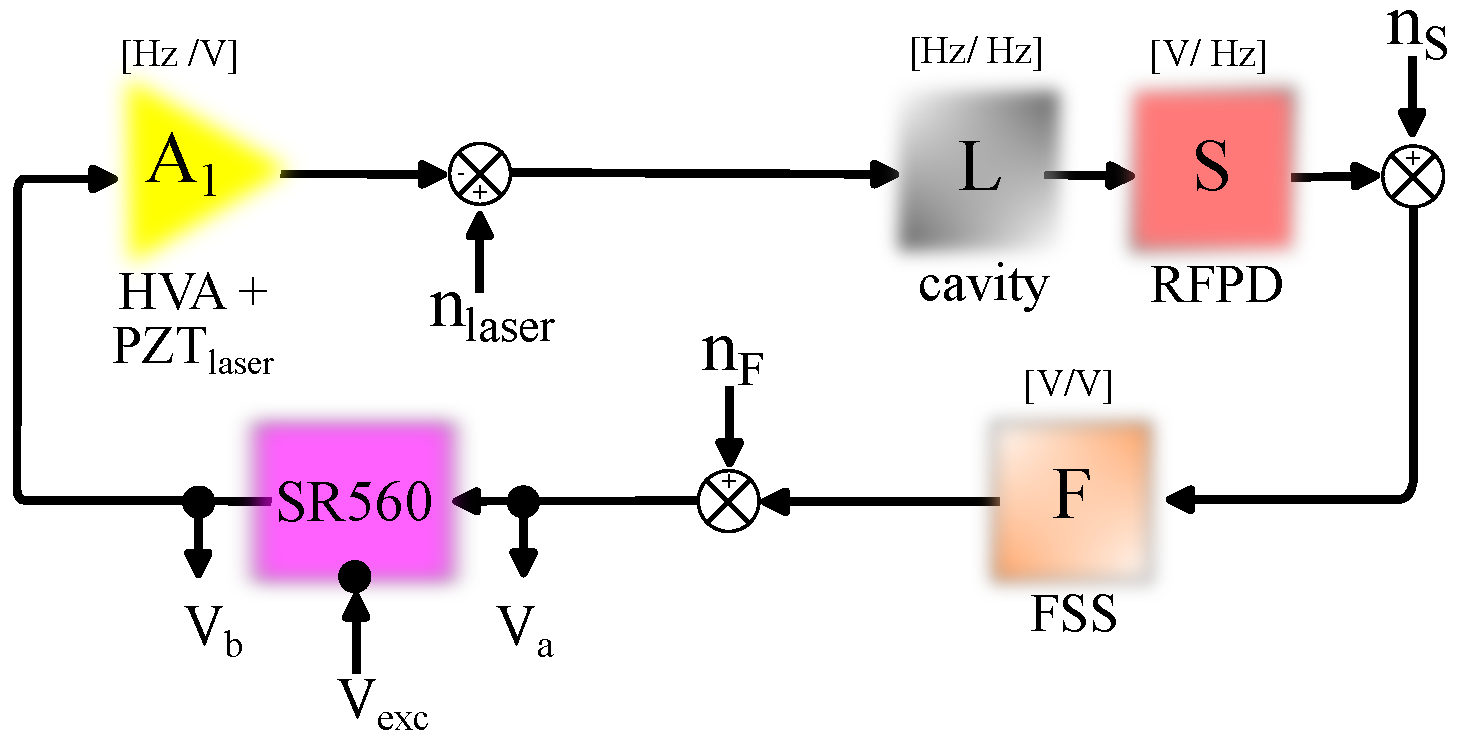
\includegraphics[width=\textwidth]{figs/ALGAAS/olg_meas_diagram.pdf}
    \caption{Open loop gain measurement diagram}
  \end{center}
  \label{fig:OLGmath}
\end{figure}

\begin{equation}
    \mathrm{V}_\mathrm{b} = (\mathrm{V}_\mathrm{exc}+n) + H(\mathrm{V}_\mathrm{exc}+n) + H^2 (\mathrm{V}_\mathrm{exc}+n) + \mathrm{H.O.T.s} = \frac{\mathrm{V}_\mathrm{exc} + n}{1-H}
\end{equation}

\begin{equation}
    \mathrm{V}_\mathrm{a} = H\cdot \mathrm{V}_\mathrm{exc} + H^2\mathrm{V}_\mathrm{exc} + H^3\mathrm{V}_\mathrm{exc} + \mathrm{H.O.T.s}  = \frac{H\mathrm{V}_\mathrm{exc}}{1-H}
\end{equation}

We take the transfer function measurement $\zeta$:

\begin{equation}
    \zeta = \frac{\mathrm{V}_\mathrm{a}}{\mathrm{V}_\mathrm{b}} = \frac{H \cdot \mathrm{V}_\mathrm{exc}/(1-H)}{(\mathrm{V}_\mathrm{exc}+n)/(1-H)}
\end{equation}

Assuming the excitation is appreciably larger than the noise ($e>>n$):

\begin{equation}
\zeta \approx H
\end{equation}

Isn't quite $\mathrm{A}(f)*\mathrm{S}(f)$ as stated. Doesn't entirely account for the optical plant.
How the measurement is taken (important to take between installations to account for the changes in the optical plant) (elog 831)

\begin{figure}[H]
\begin{center}
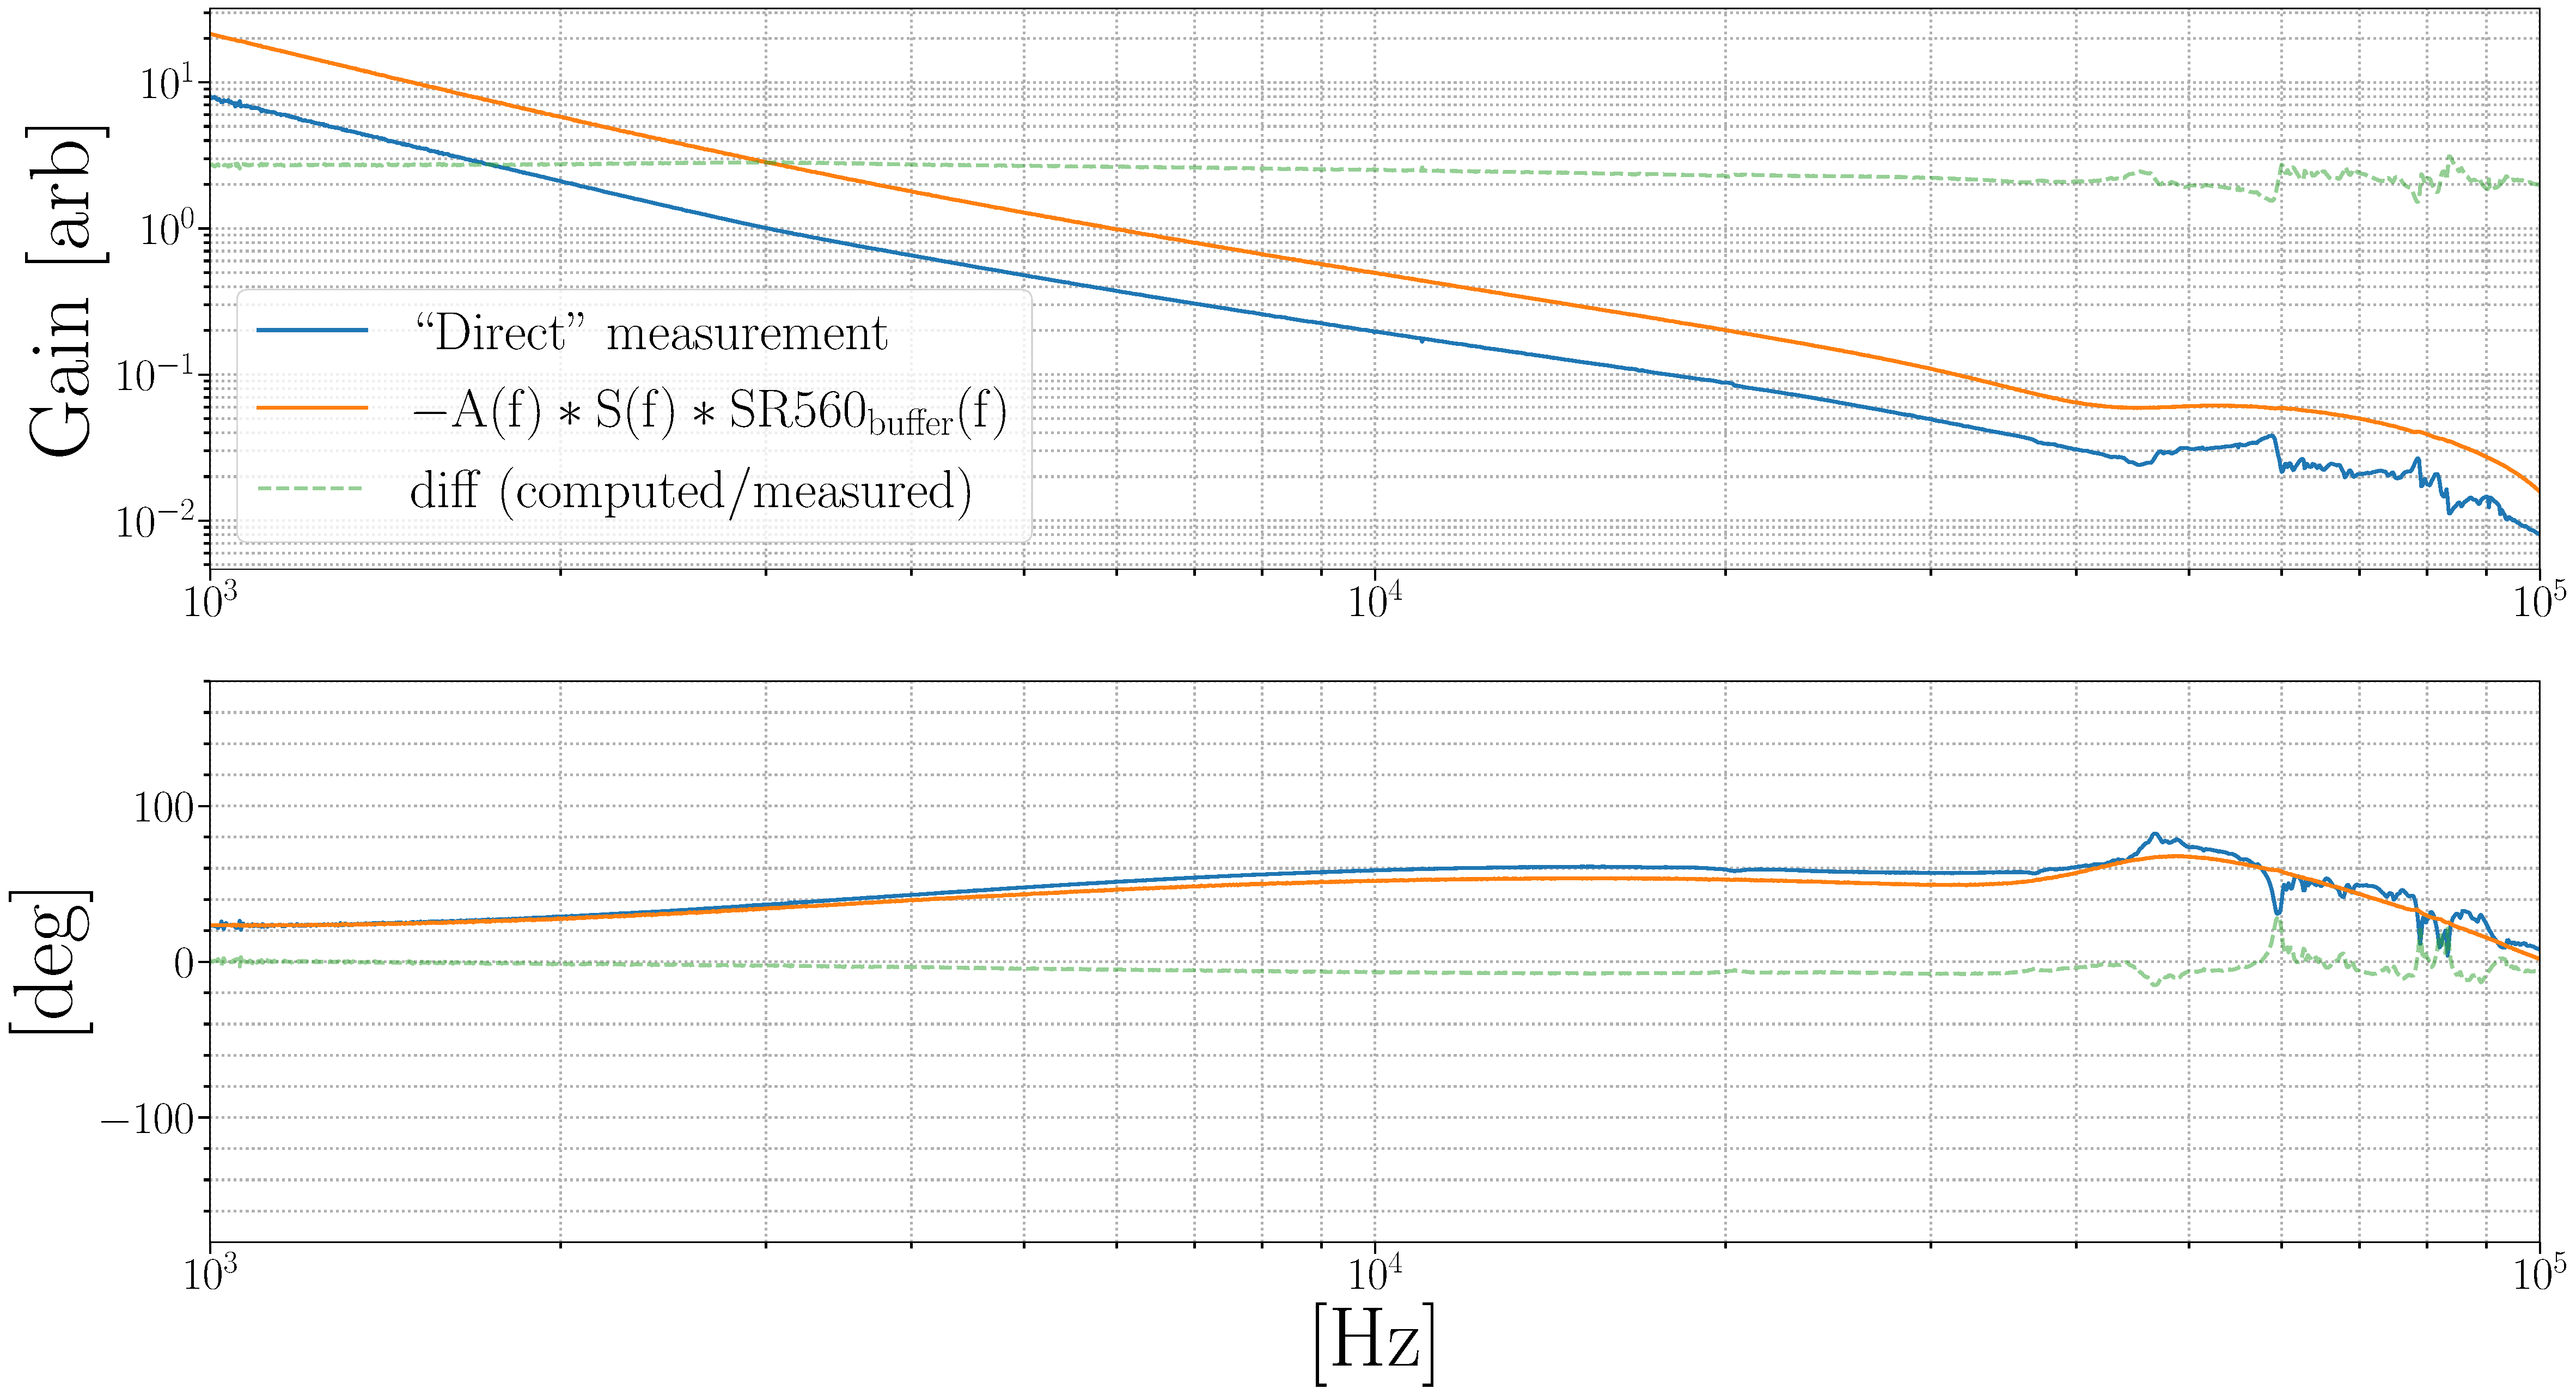
\includegraphics[width=\textwidth]{ALGAAS/olg_compare.pdf}
\end{center}
\caption{Comparison of the open loop gain measurement against the multiplied servo electronics measurements. The maximum gain difference is about a factor of 2.8 which is low passed to a difference of 2.0.}
\label{fig:OLGcompare}
\end{figure}

\newpage

\section{Alternate Mounting Solutions (Assemblies \texorpdfstring{$1 \rightarrow 3$}{1to3})}\label{appendix:mount_assemblies}

\section{Assembly blueprints and alternative views}

\subsection{Assembly 0 and 1}

\subsubsection*{Model params}
\begin{center}
\begin{tabular}{ |c|c|c|c|c|c| } 
\hline
$\mathrm{r}_{ap}$ [m] &  $\mathrm{t}_{cap}$ [m] & $\mathrm{r}_{el}$ [m] & $\mathrm{t}_{el}$ [m] & $\mathrm{r}_{opt}$ [m] & $\mathrm{t}_{opt}$ [m] \\
\hline
1.5e-3 & 4.5e-3 & 38.1e-3 & 1.5e-3 & 12.7e-3 & 6.35e-3 \\ 
\hline
\end{tabular}
\end{center}

\subsubsection*{Electrodes}
\begin{figure}[H]
  \centering
  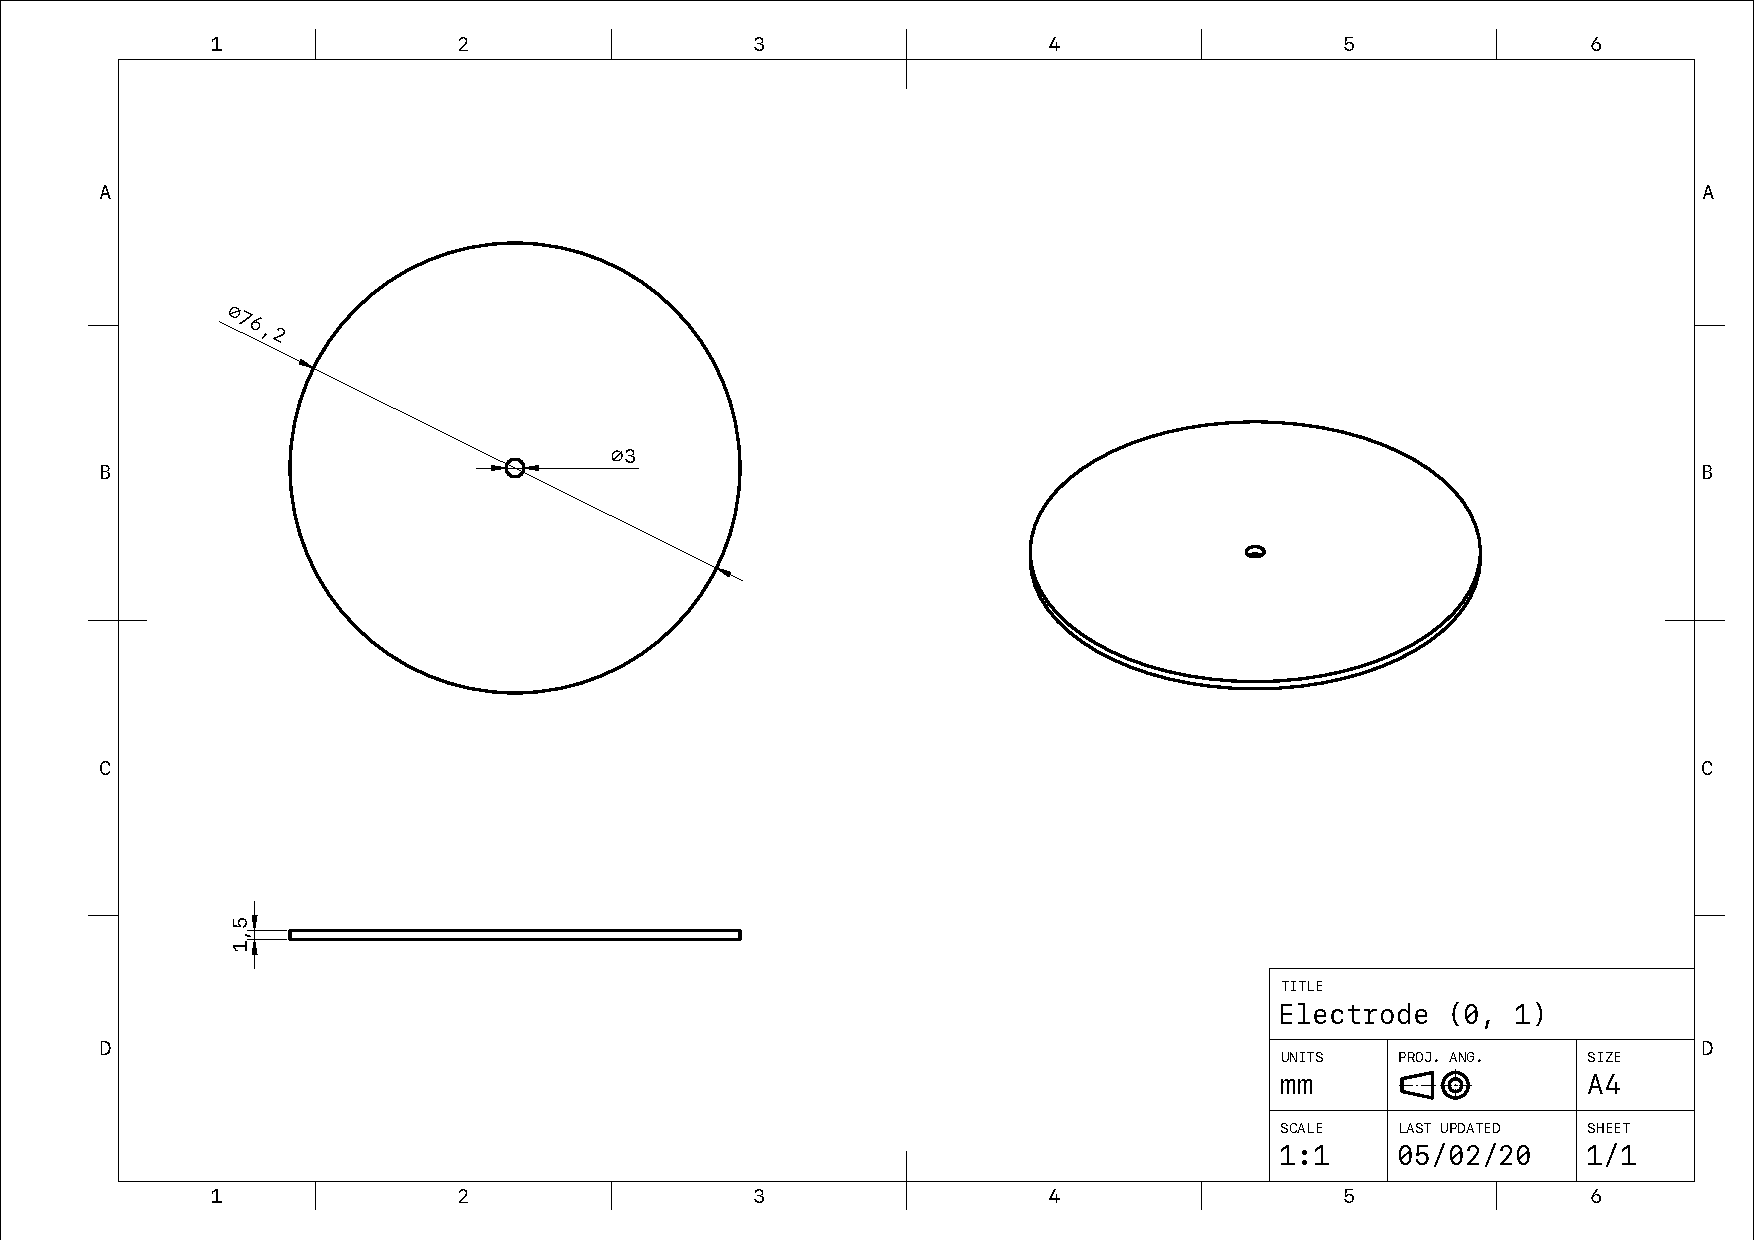
\includegraphics[width=\textwidth]{figs/ALGAAS/assemblies/assembly0/Electrode_0_1.pdf}
  \caption{Technical drawing of the 3" disk electrode plates made of aluminum.}
\end{figure}

\subsubsection*{Mount 0}

\begin{figure}[!ht]
	\begin{subcaptiongroup}
		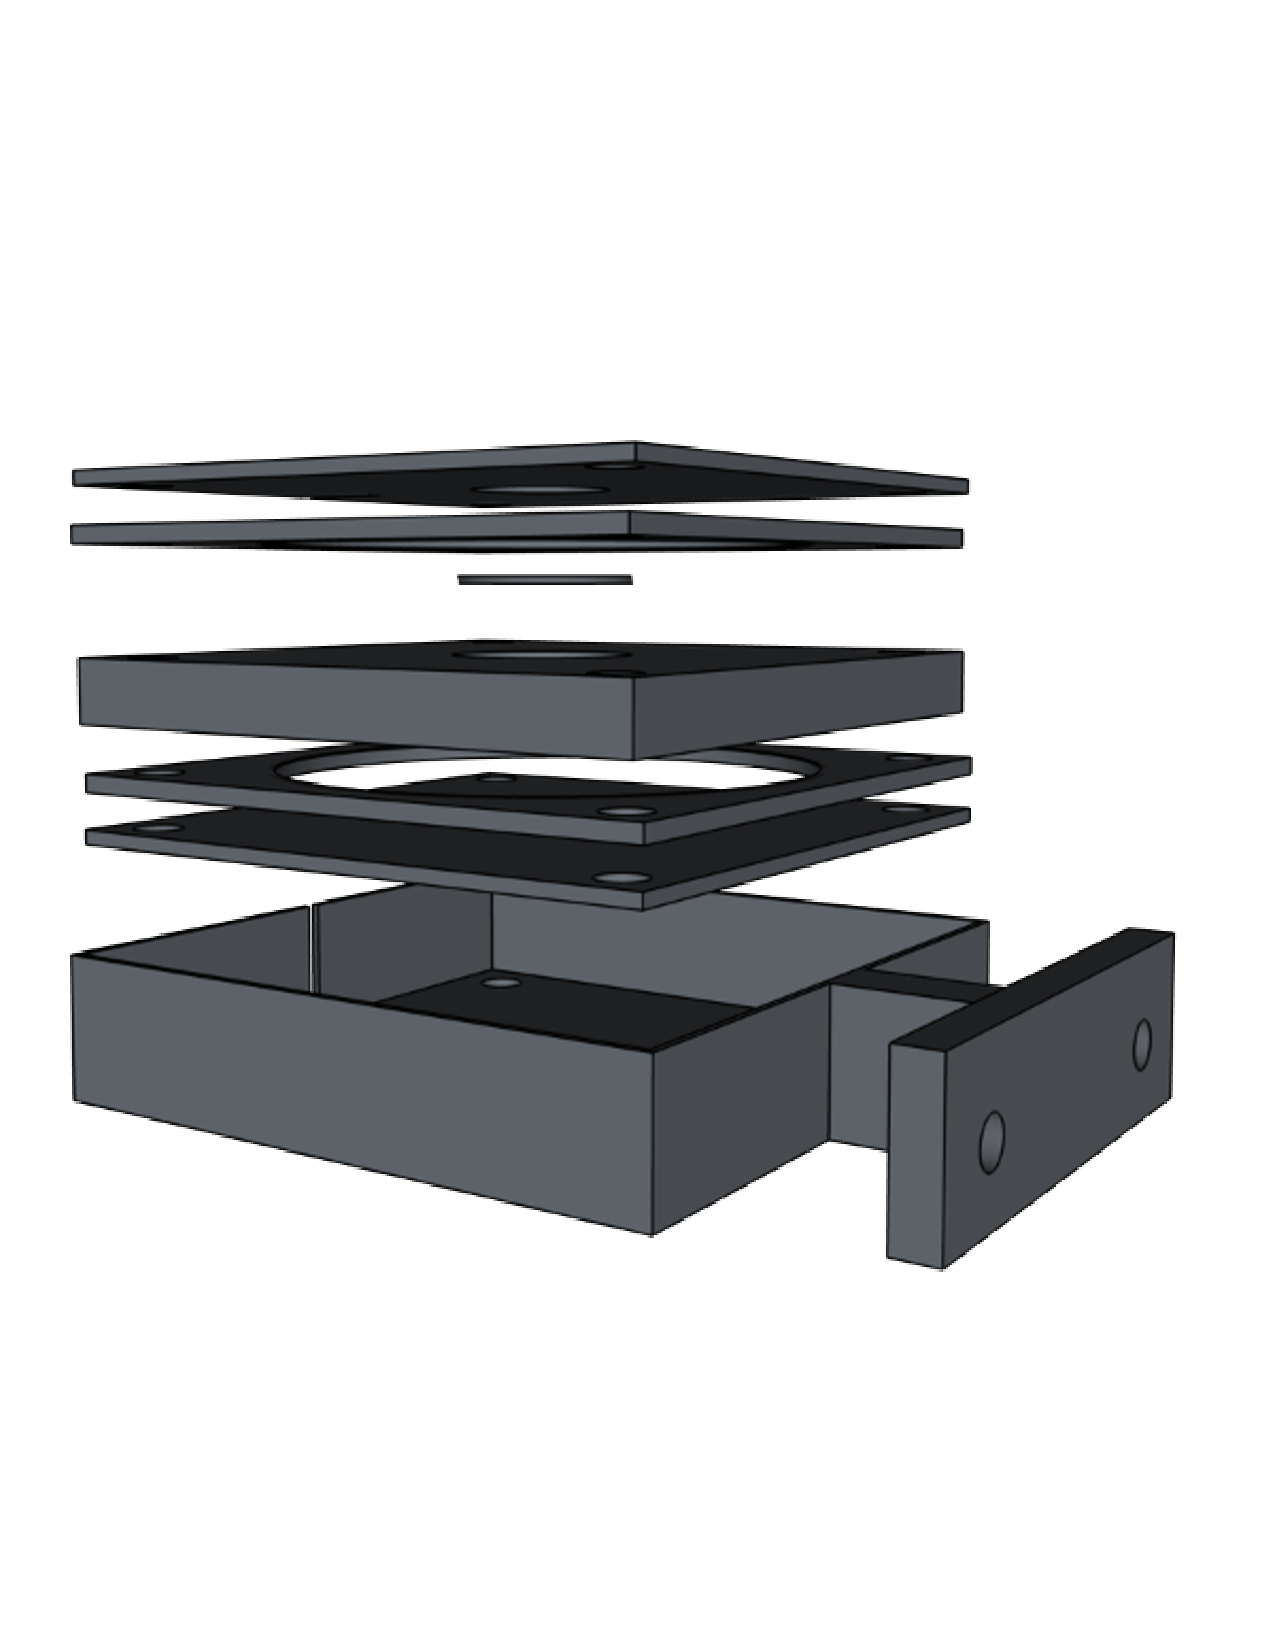
\includegraphics[width=.5\textwidth]{figs/ALGAAS/assemblies/assembly0/assembly0.pdf}
		\phantomcaption\label{A0}
		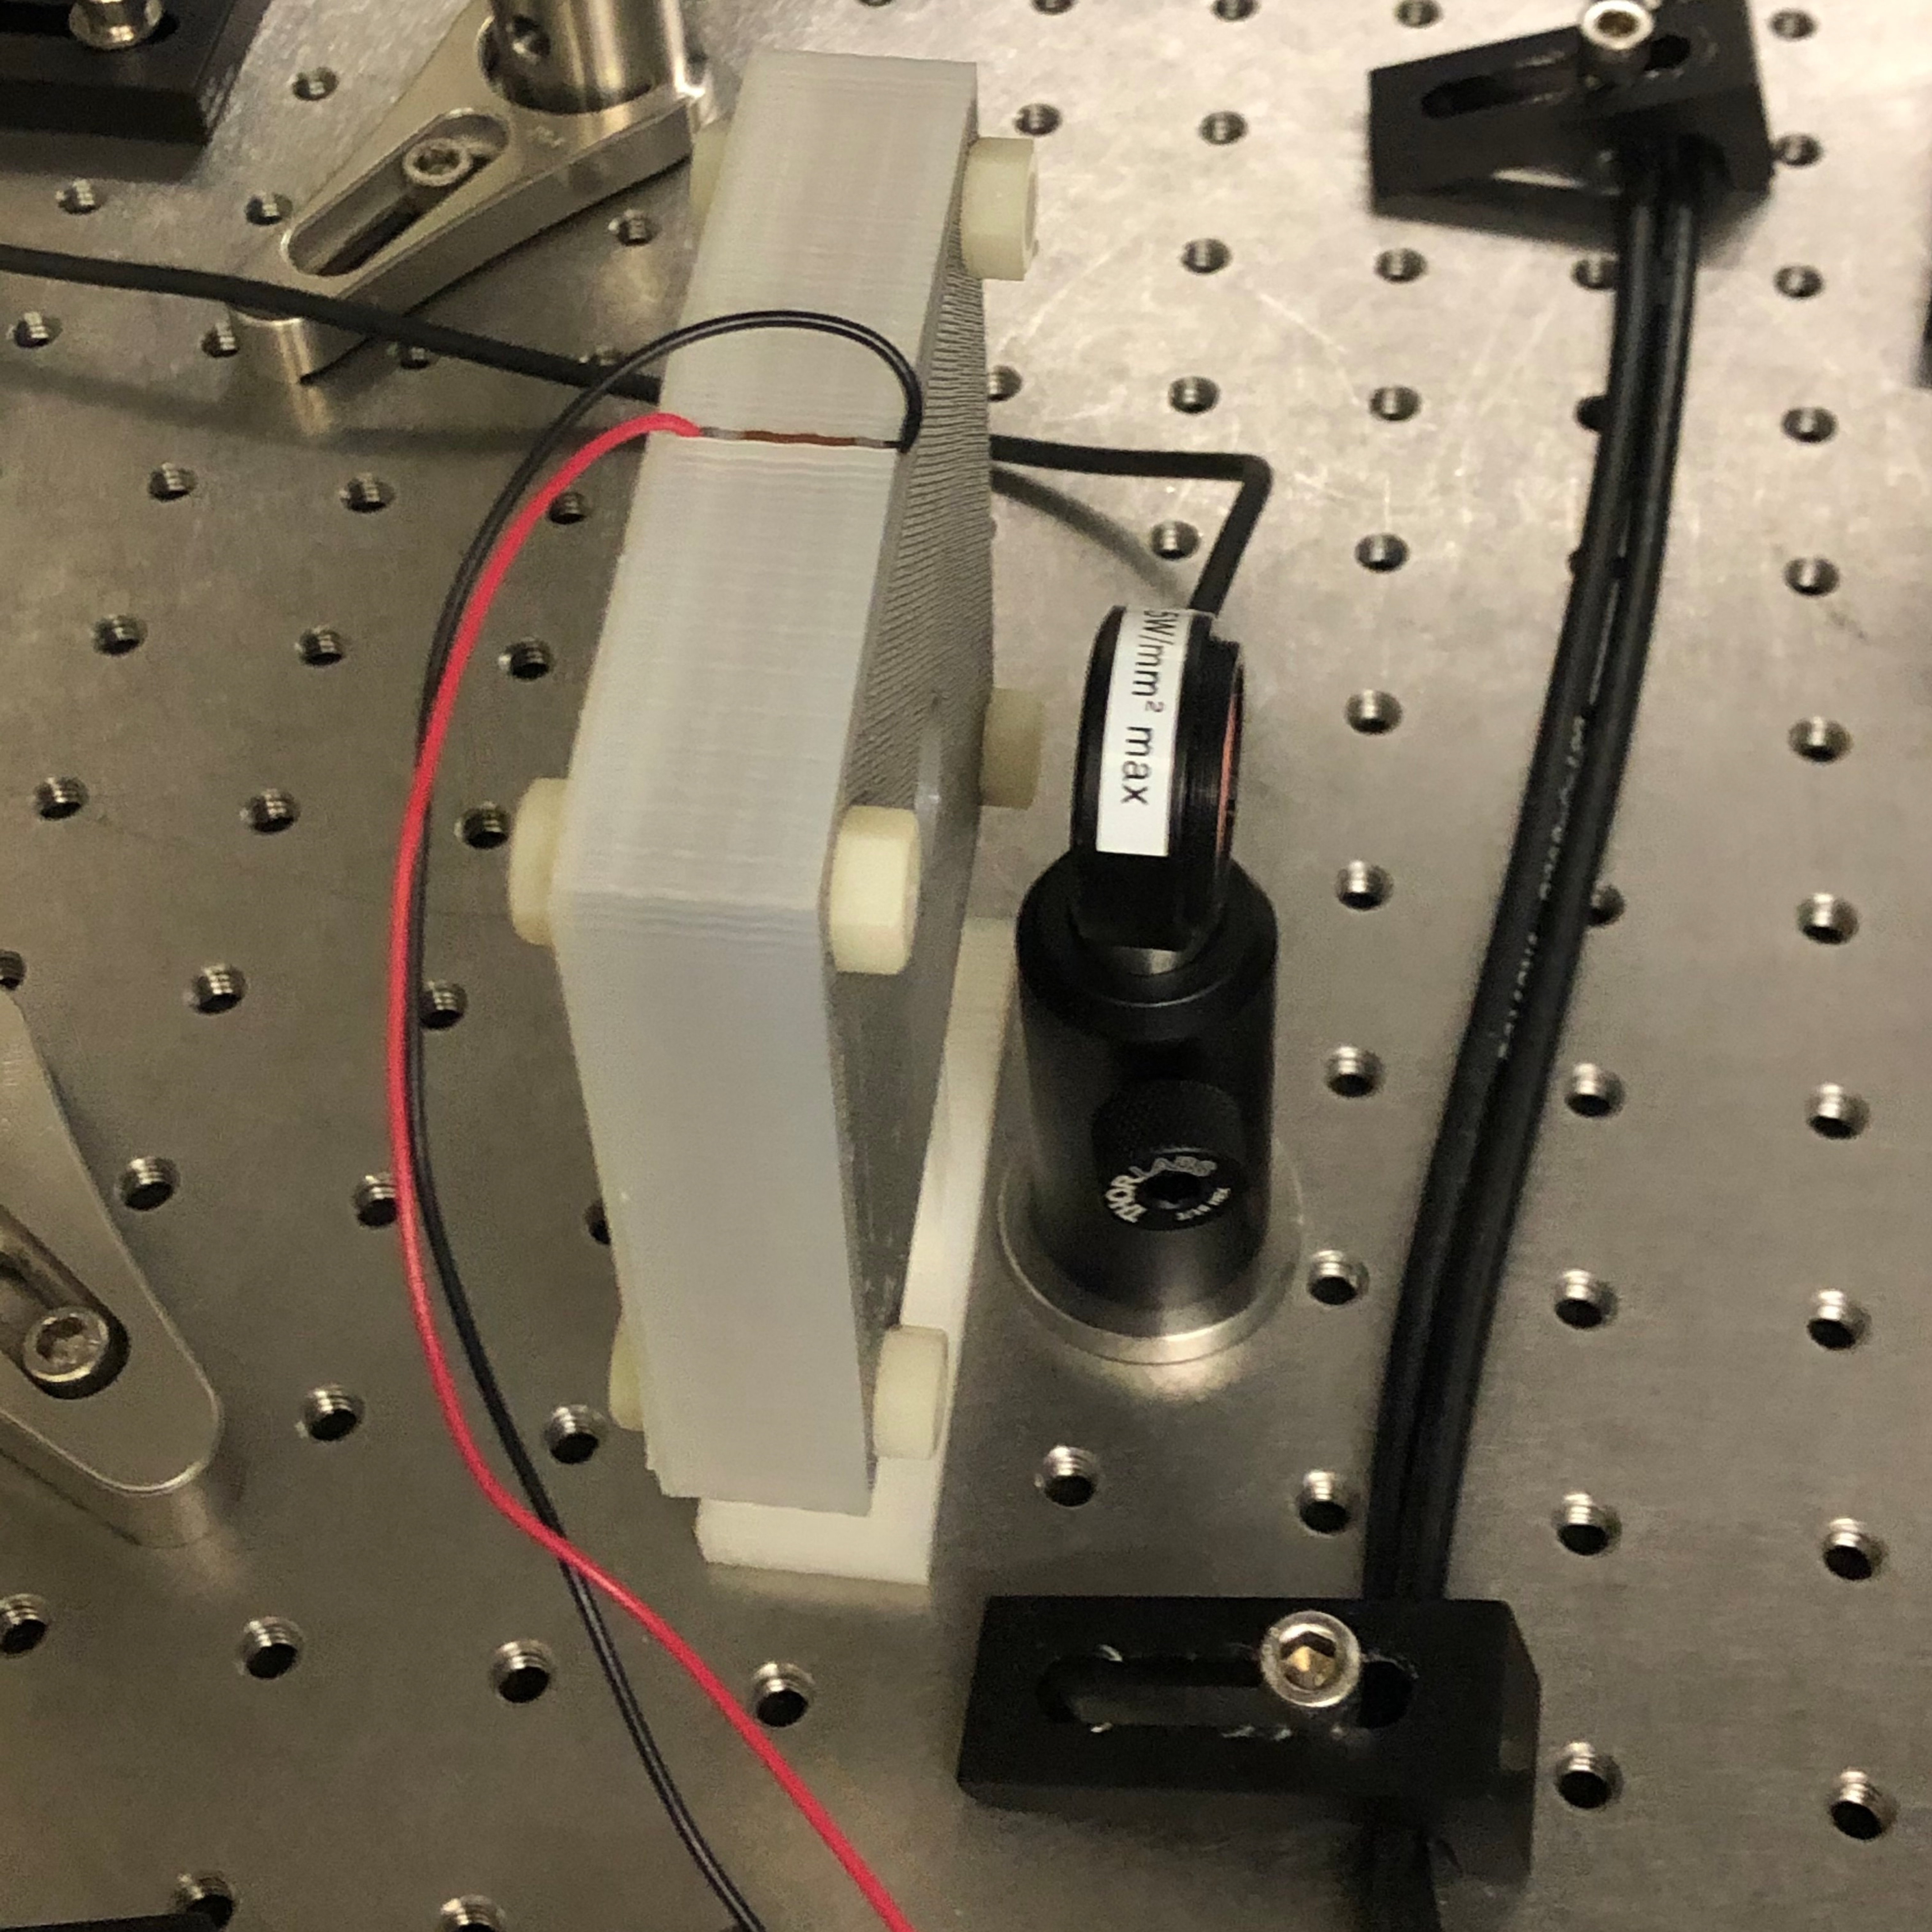
\includegraphics[width=.5\textwidth]{figs/ALGAAS/assemblies/assembly0/assembly0_incident_power.pdf}
 		\phantomcaption\label{A0inc}
	\end{subcaptiongroup}
  \caption{Assembly 0 was constructed to meet the criteria of providing a non-conductive housing for the electrode / sample assembly while maintaining a fixed length spacing using parts 3d printed with polylactic acid filament (PLA).}
  \label{fig:assembly0bp}
\end{figure}
\FloatBarrier

\subsubsection*{Mount 1.1}
\begin{figure}[!ht]
	\begin{subcaptiongroup}
		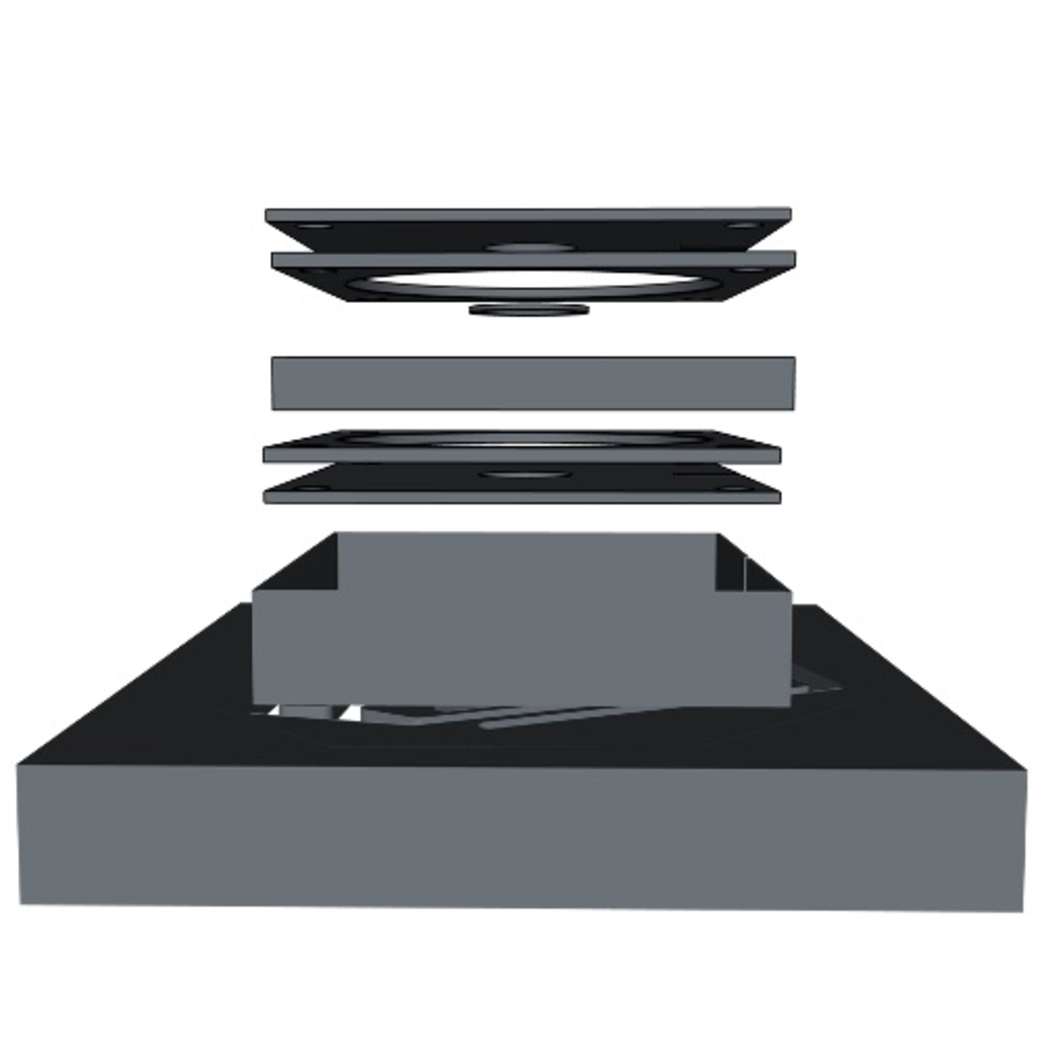
\includegraphics[width=.49\textwidth]{figs/ALGAAS/assemblies/assembly1/assembly1_dissassembled.pdf}
		\phantomcaption\label{A1pt2CAD}
		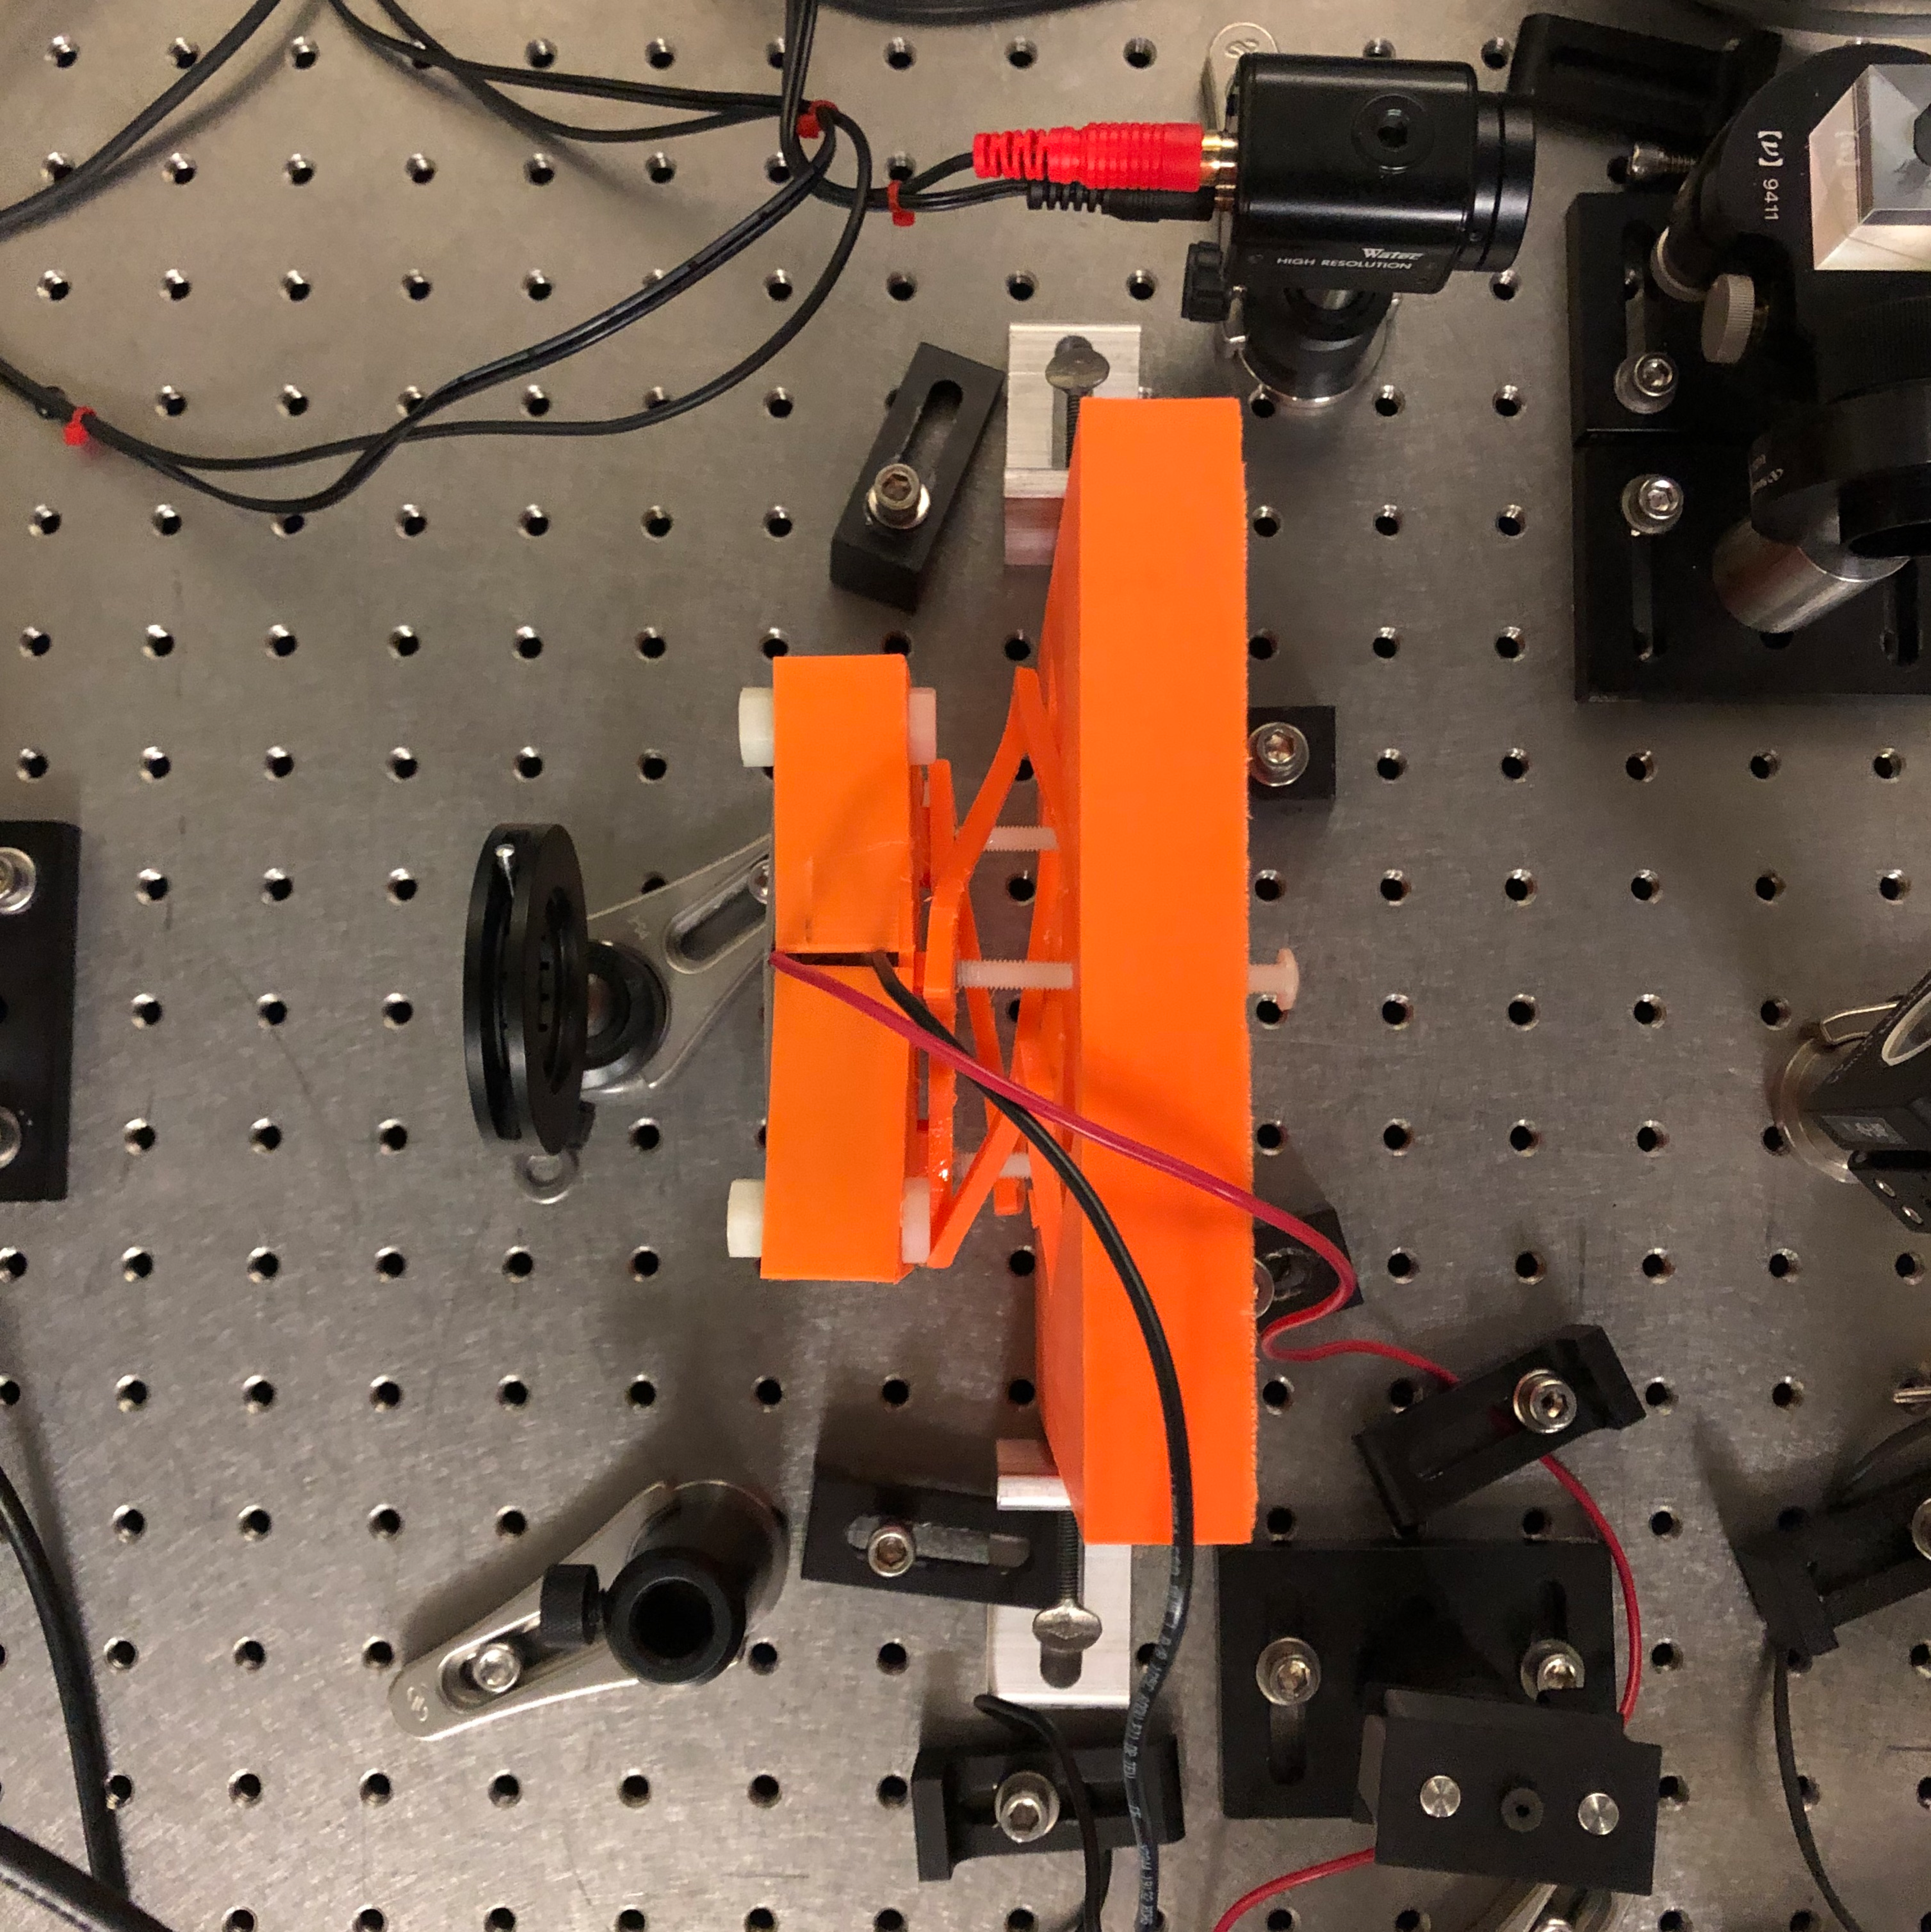
\includegraphics[width=.49\textwidth]{figs/ALGAAS/assemblies/assembly1/assembly1_insitu2.pdf}
		\phantomcaption\label{A1pt2pic}	
	\end{subcaptiongroup}
	\caption{Assembly 1 was constructed to meet the criteria of providing a non-conductive housing for the electrode / sample assembly while maintaining a fixed length spacing using parts 3d printed with polylactic acid (PLA).}
	\label{fig:assembly1bp}
\end{figure}
\FloatBarrier

\subsubsection*{Mount 1.2}
\begin{figure}[!ht]
	\begin{subcaptiongroup}
		\includegraphics[width=.5\textwidth]{figs/ALGAAS/assemblies/assembly1/assembly1_mod_front.pdf}
		\phantomcaption\label{A1pt3CAD}
		\includegraphics[width=.5\textwidth]{figs/ALGAAS/assemblies/assembly1/assembly1_mod_side.pdf}
		\phantomcaption\label{A1pt3pic}
	\end{subcaptiongroup}
	\caption{A modification implemented with the intention of reducing pitch dithering while still having control of DC YAW}
	\label{fig:assembly1mod}
\end{figure}

\newpage

\subsubsection*{Tests and commentary}

\begin{figure}[!ht]
    \begin{subcaptiongroup}
	    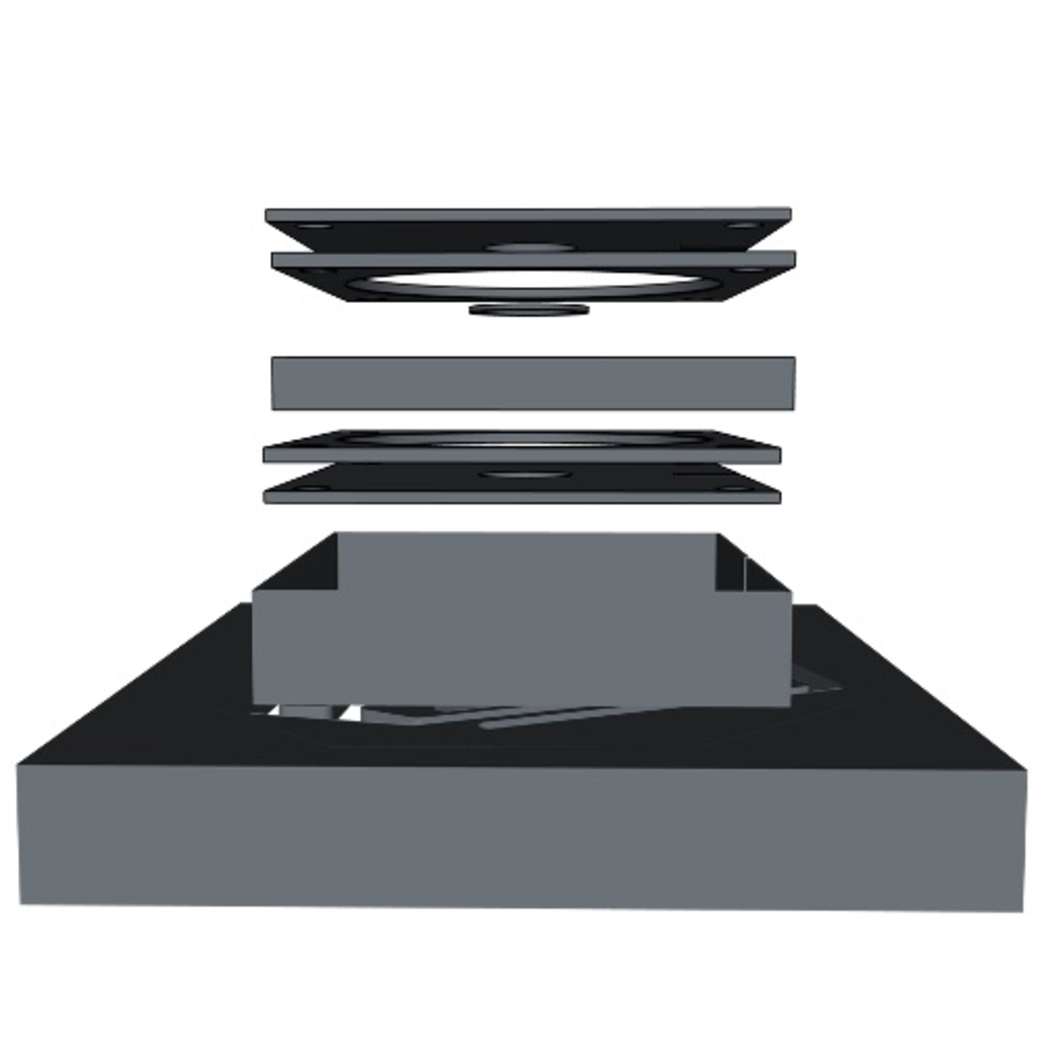
\includegraphics[width=.5\textwidth]{figs/ALGAAS/assemblies/assembly1/assembly1_dissassembled.pdf}
	    \phantomcaption\label{A1disassembled}
	    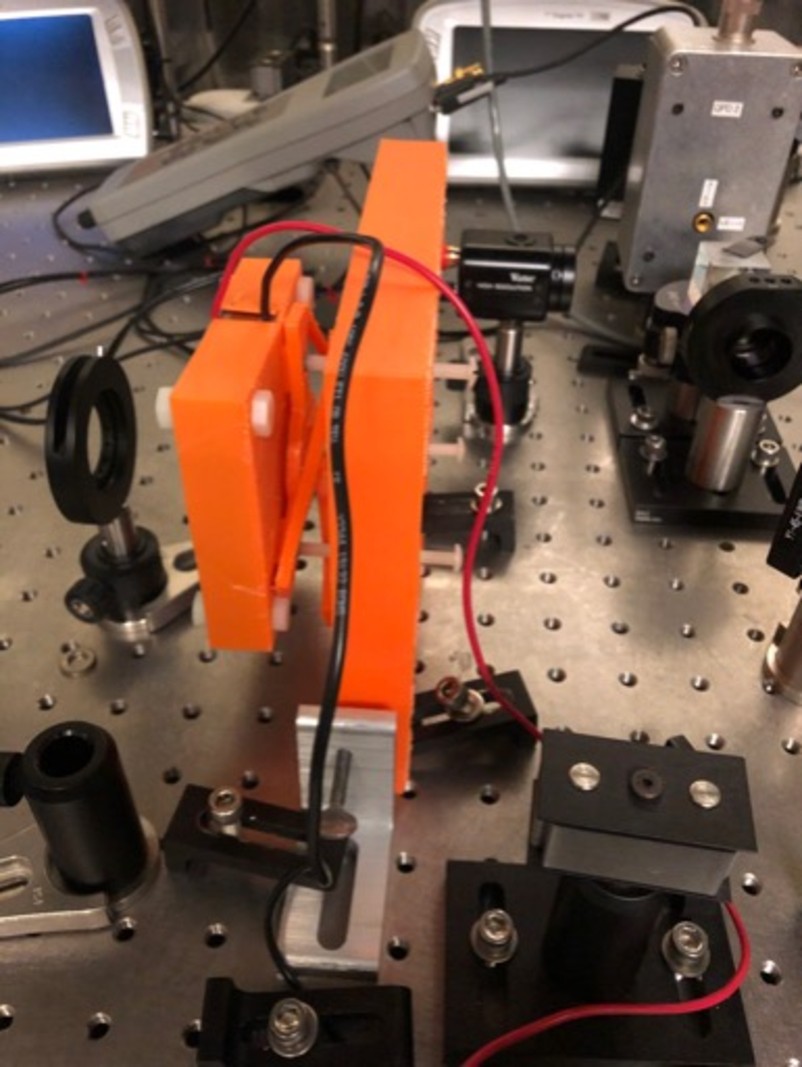
\includegraphics[width=.5\textwidth]{figs/ALGAAS/assemblies/assembly1/assembly1_flaw.pdf}
	    \phantomcaption\label{A1flaw}
    \end{subcaptiongroup}
    \caption{Assembly 1 was constructed to meet two criteria: the same solution of housing the sample and electrodes as Assembly 0, but also offer pitch / yaw control via an ortho-planar spring design (Brigham Young University).}
    \label{fig:A1pt0}
\end{figure}
\FloatBarrier


The construction revealed flaws; made most obvious when comparing to displacement noise of traditional optical mounts. Pitch and yaw control via the ortho-planar spring were prioritized to avoid metal springs and further mount pieces. The solution became unjustifiable when observing the the displacement noise coupling from the mount.

%%Re-run this calibration with adequate voltage normalization for a response unit [$m_\mathrm{pk} / [V / m]$]

\begin{figure}[H]
\centering
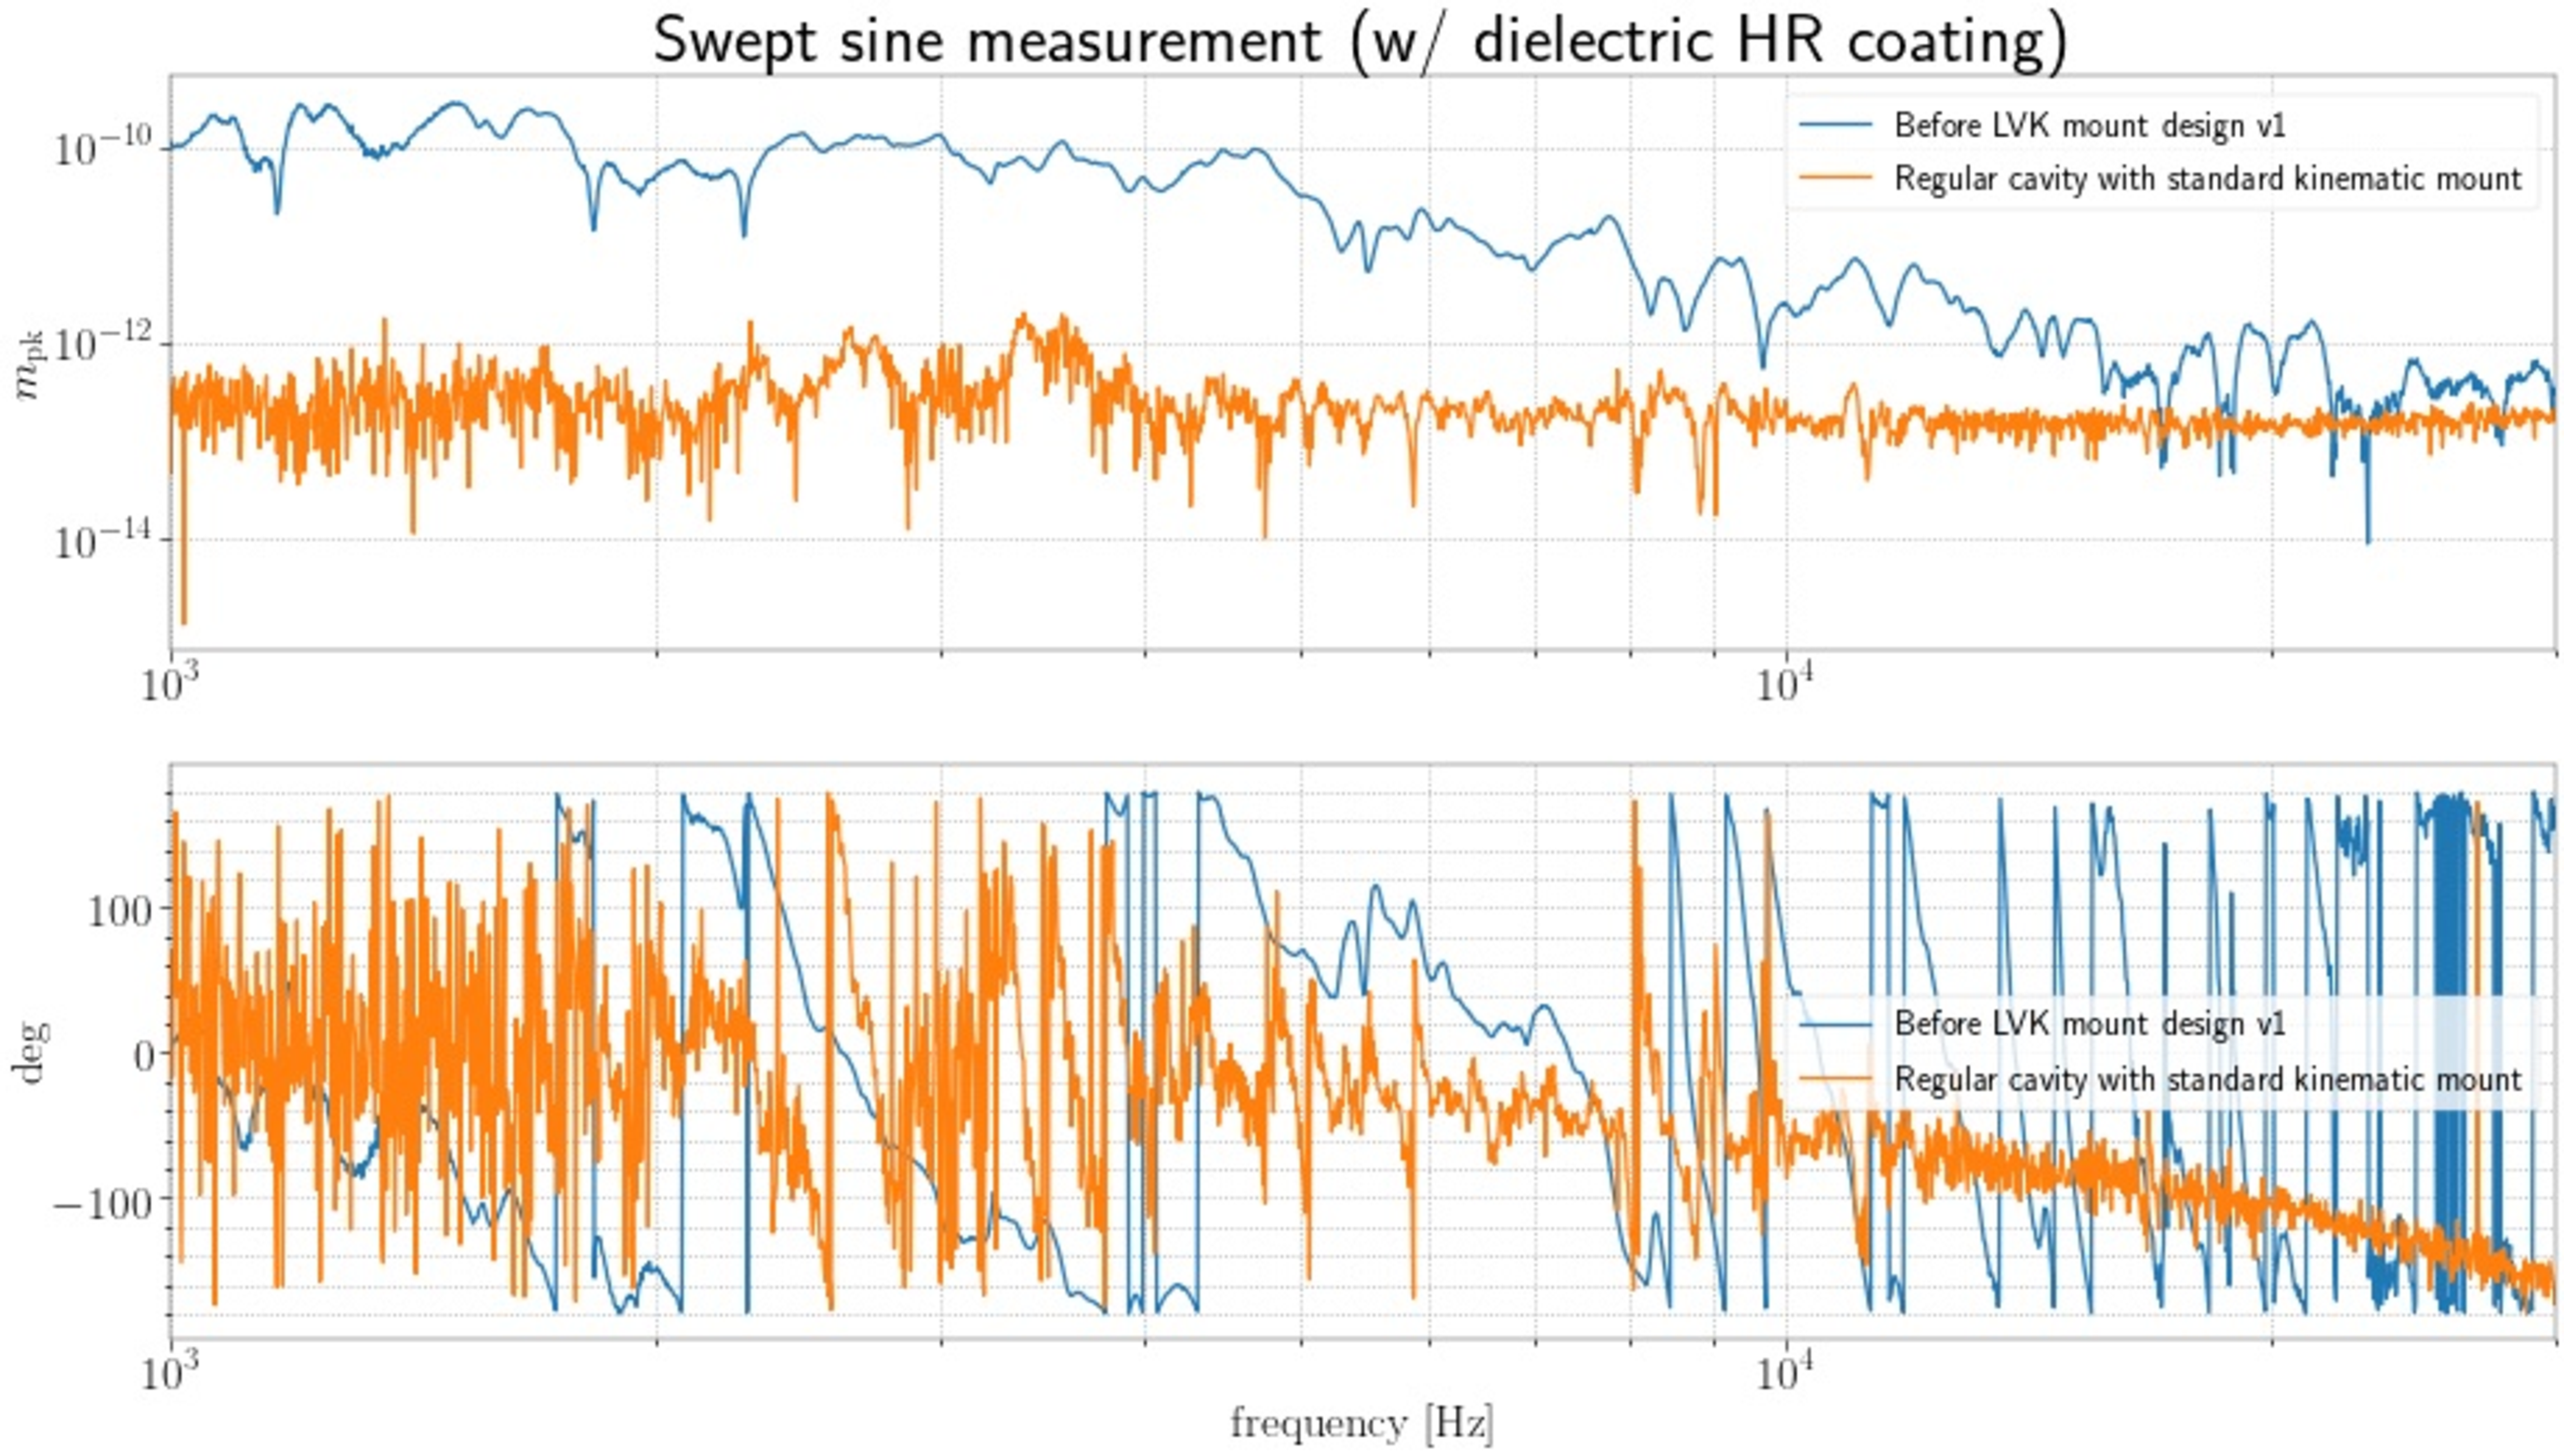
\includegraphics[width=\textwidth]{figs/ALGAAS/assemblies/assembly1/assembly1_2_compare_standmount.pdf}
\caption{Measured displacement spectra for Assembly 1.2 of the longitudinal pockels cell mount compared to the standard kinematic mount. Both measurements were recorded with the the CVI Melles-Griot (amorphous) mirror coating sample installed in the assembly.}
%%Units and legend labels need increase in font size. Remove Swept sine measurement title.
\label{fig:A12cmpkinmnt}
\end{figure}

\begin{figure}[H]
    \centering
    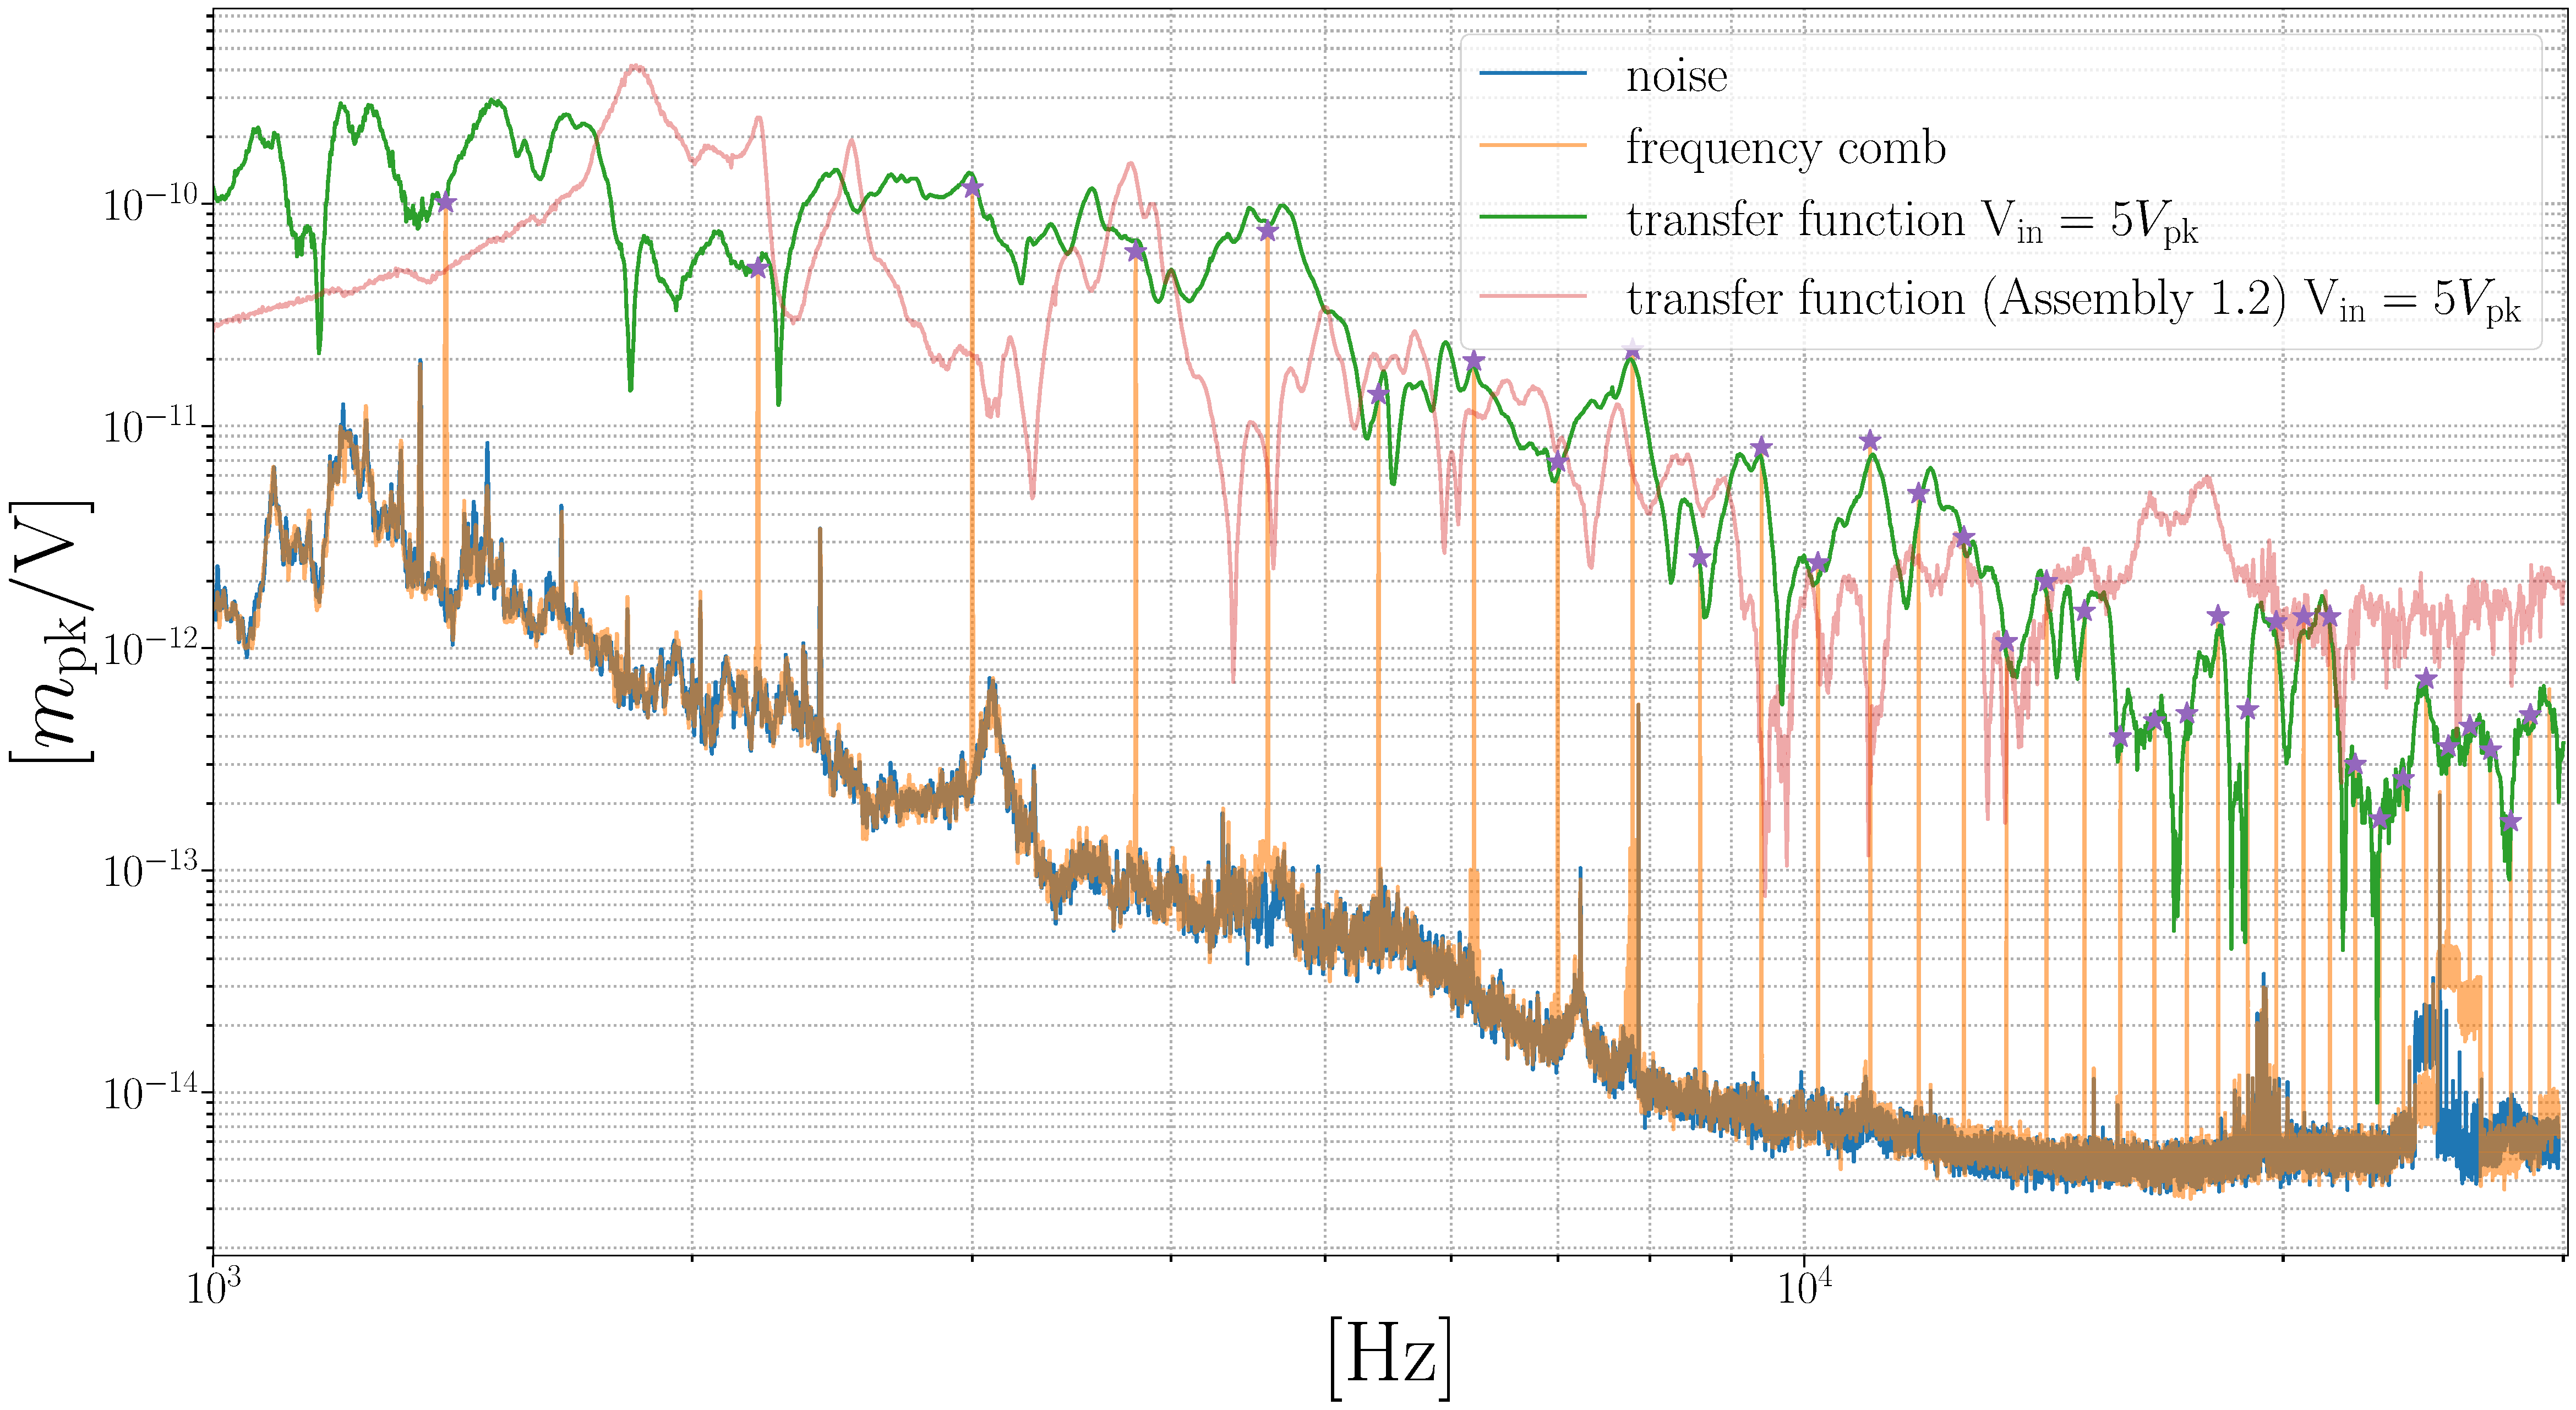
\includegraphics[width=.92\textwidth]{figs/ALGAAS/results_figs/assembly1/1_2_cvi_compare_tfwcmb.pdf}
    \caption{Assembly 1.2 and 1.3 transfer function measurement and separate noise displacement spectra measurement with a CVI Melles Griot flat mirror sample ($R \approx $ sample installed. Measurements were taken from 1kHz up to 30kHz on using a Stanford Research 785 spectrum analyzer.}
    \label{fig:assembly12and13displacementspectracvi}
\end{figure}


\newpage

\subsection{Assembly 2}
\subsubsection*{Model Params}
\begin{center}
\begin{tabular}{ |c|c|c|c|c|c| } 
\hline
$\mathrm{r}_{ap}$ [m] &  $\mathrm{t}_{cap}$ [m] & $\mathrm{r}_{el}$ [m] & $\mathrm{t}_{el}$ [m] & $\mathrm{r}_{opt}$ [m] & $\mathrm{t}_{opt}$ [m] \\
\hline
1.5e-3 & 12.7e-3 & N/A (rectangular) & 1.27e-3 & 12.7e-3 & 6.35e-3 \\ 
\hline
\end{tabular}
\end{center}

\subsubsection*{Electrodes}

\begin{figure}[H]
  \centering
  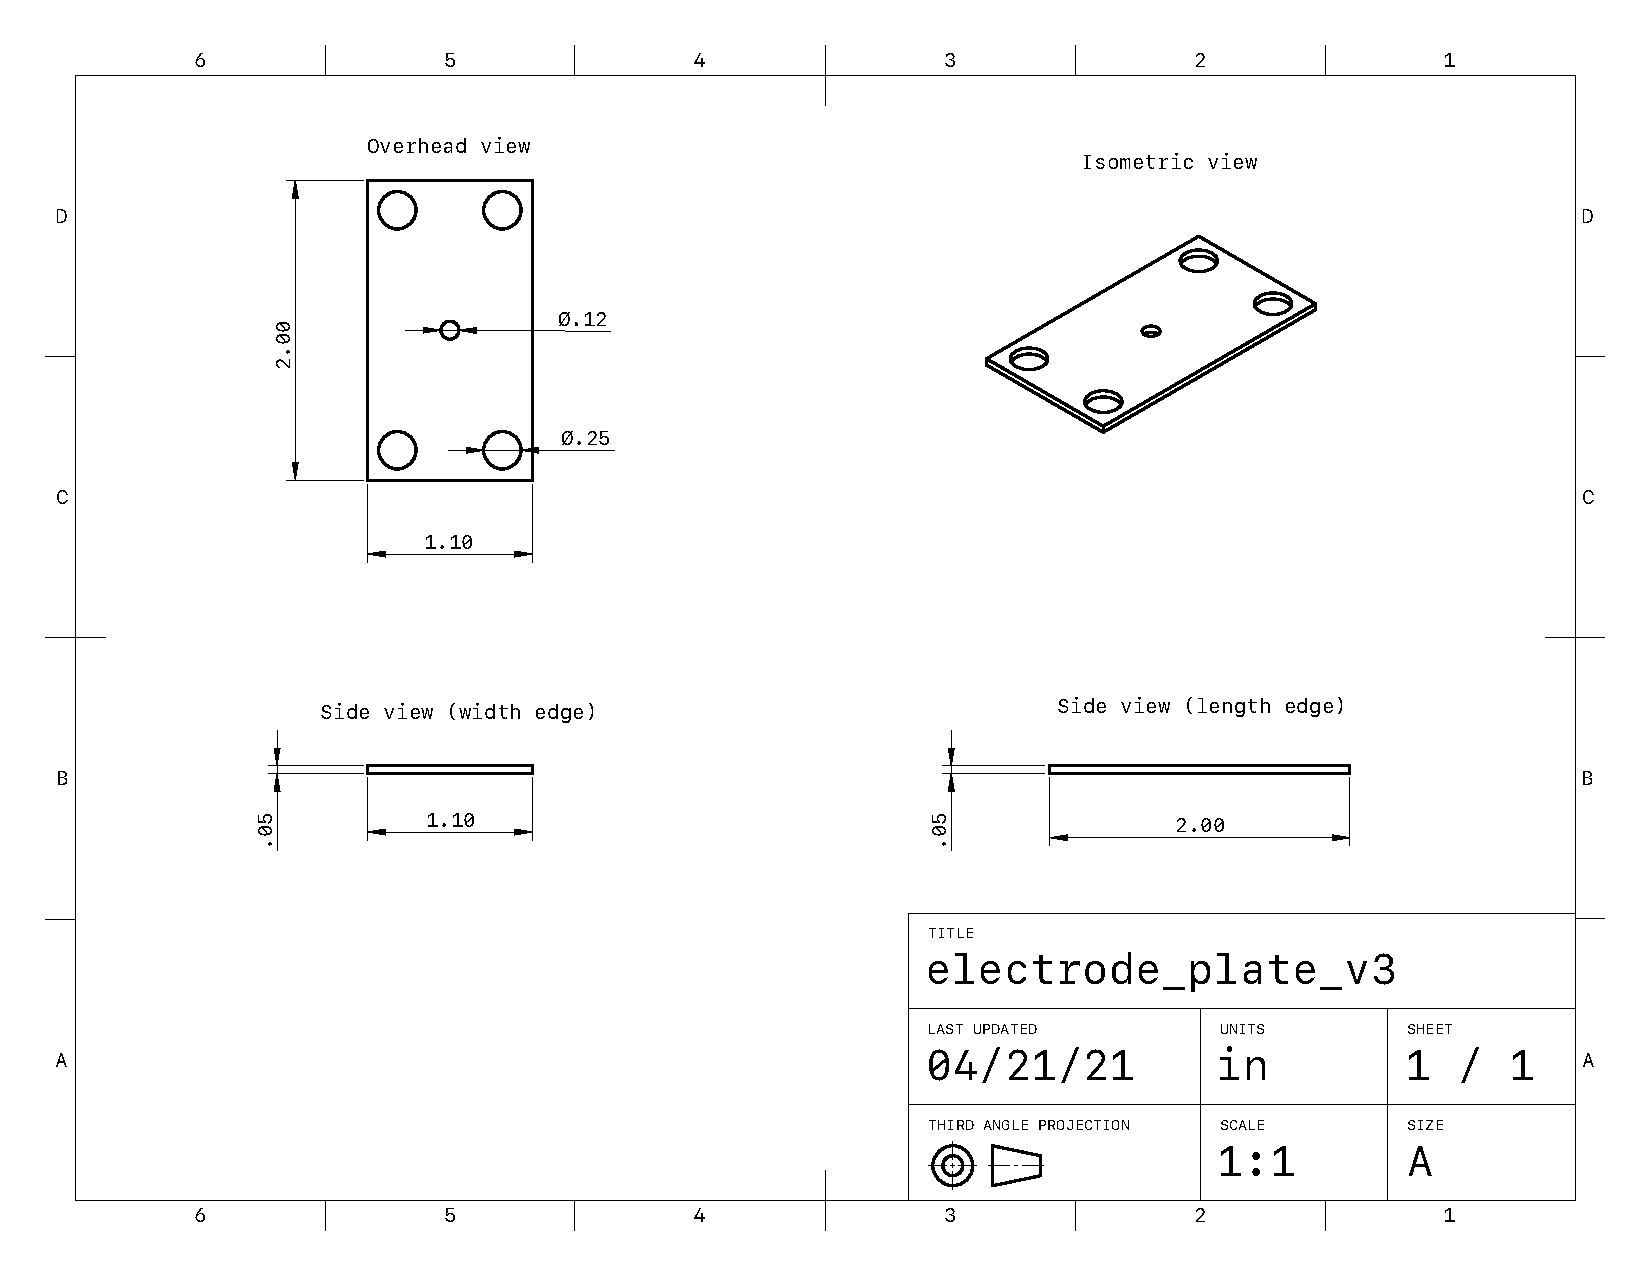
\includegraphics[width=\textwidth]{figs/ALGAAS/assemblies/assembly2/assembly2_electrode.pdf}
  \caption{Rectangular (.05"X1.1"X2") plates made of aluminum.}
\end{figure}

\newpage

\subsubsection*{Mount 2.0}
\begin{figure}[H]
	\centering
	\begin{subcaptiongroup}
		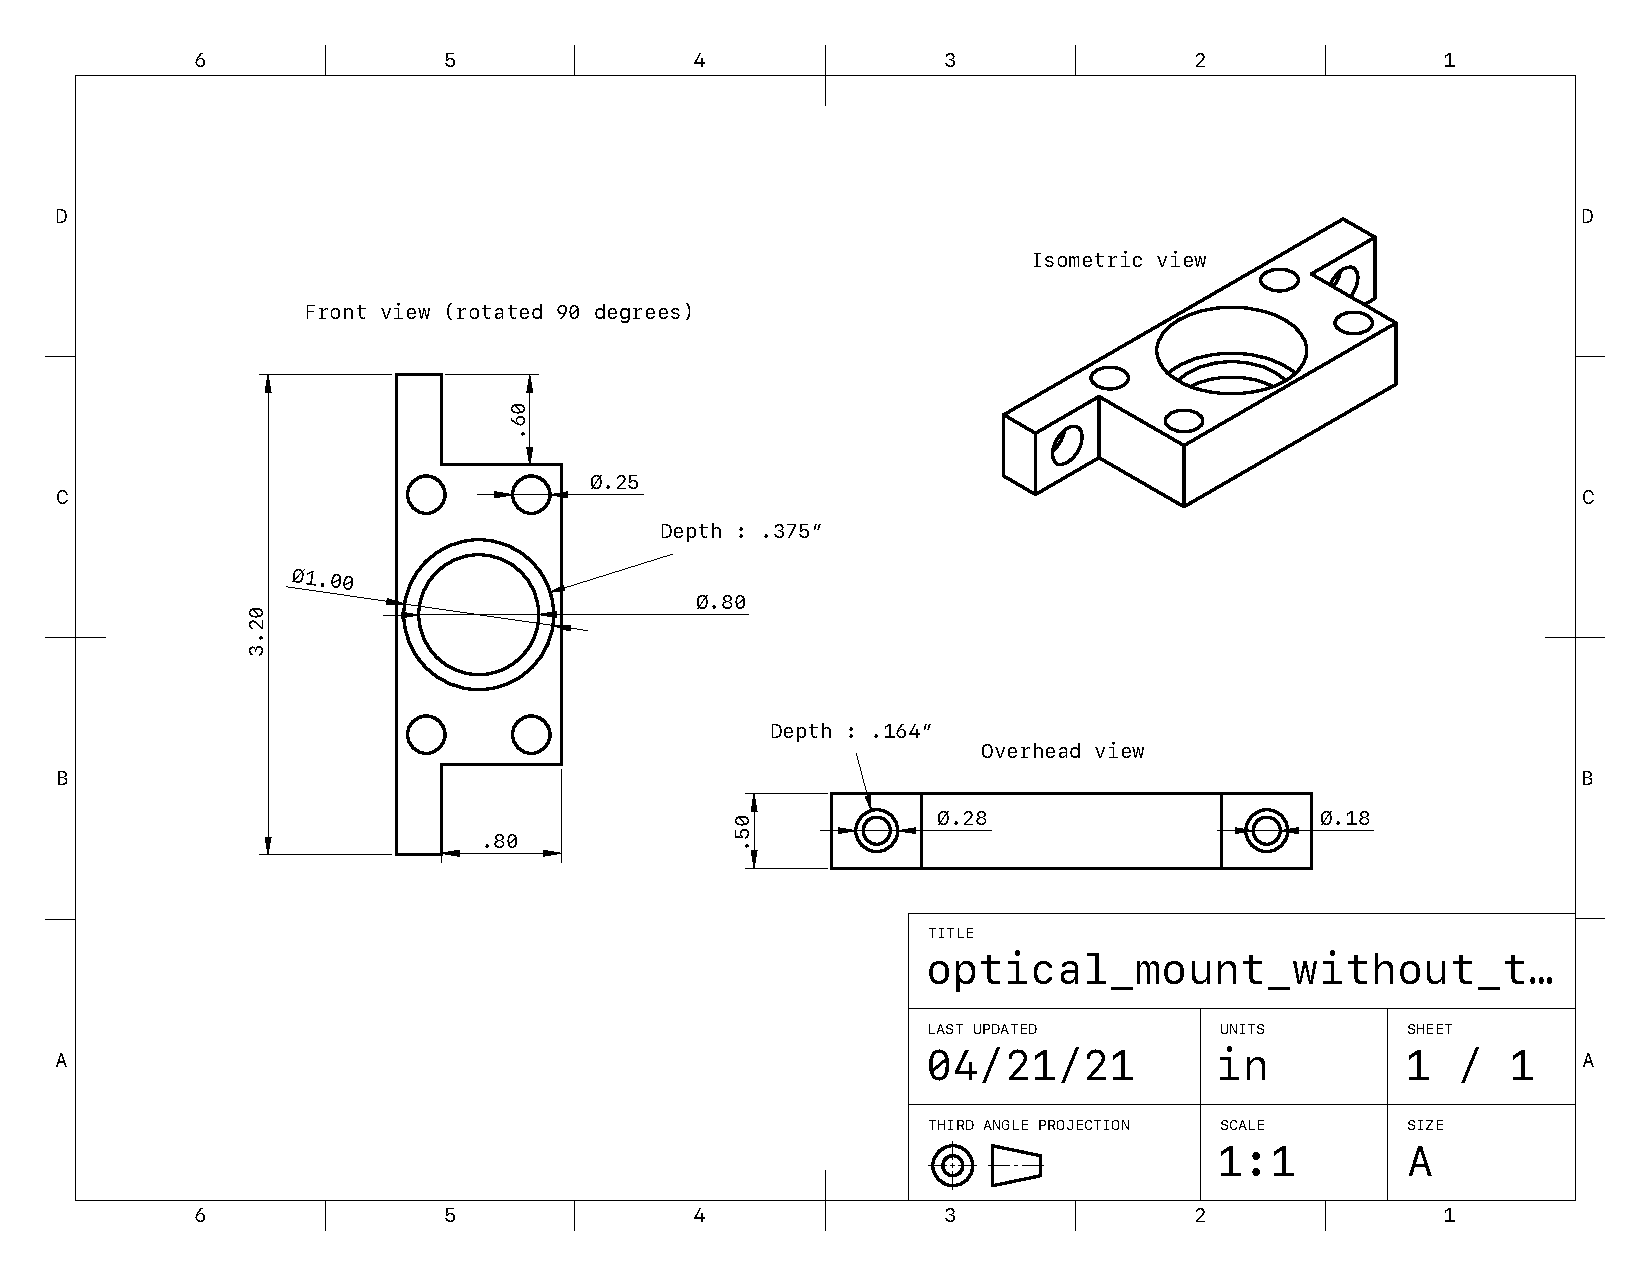
\includegraphics[width=.76\textwidth]{figs/ALGAAS/assemblies/assembly2/assembly2_PVC_mount.pdf}
		\phantomcaption\label{A2PVCmount}
		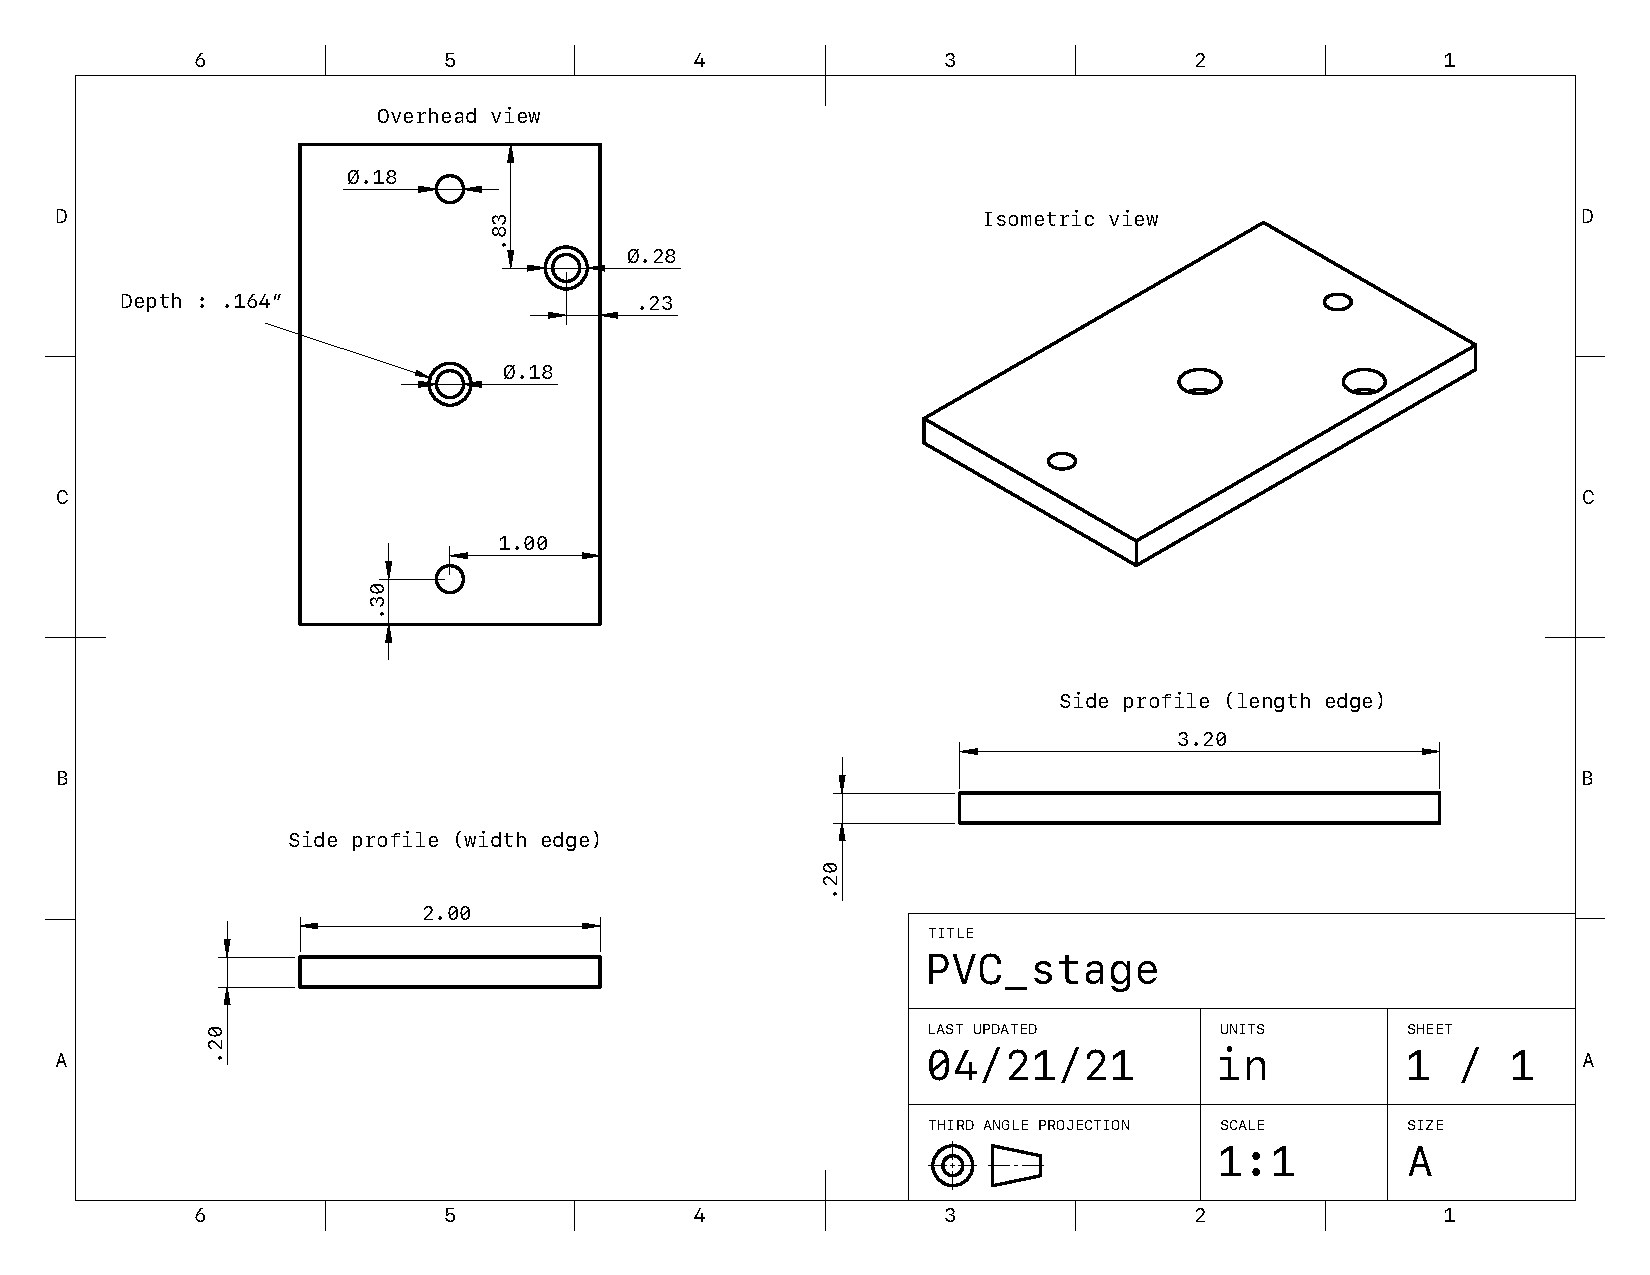
\includegraphics[width=.76\textwidth]{figs/ALGAAS/assemblies/assembly2/assembly2_PVC_stage.pdf}
		\phantomcaption\label{A2PVCstage}
	\end{subcaptiongroup}
	\caption{A design iteration of the assembly 2 mounts. Materials tried varied from PVC, PLA, and PETG. Quarter inch holes are bored in order to pass nylon screws holding electrode plates fixed to the mount.}
	\label{fig:assembly2bp}
\end{figure}
\FloatBarrier

\subsubsection*{Voltage drive tests}
With considerations after Assembly 1, a more monolithic optical mount design with a simple geometry was imagined. PLA material compliance factoring to the seen drive noise. To see if it could be due to the compliance of the assembly material or printing, we tested this assembly design against different infills of PLA, PETG, and a version machined from solid PVC. With this modification, came also a different plate geometry. The assumption is the region of interest of the injection would not be heavily influenced by the non-circular plate geometry where it matters.

% Some citations:
%\cite{PINTO2015635}

%\begin{figure}[!ht]
%	\begin{subcaptiongroup}
%		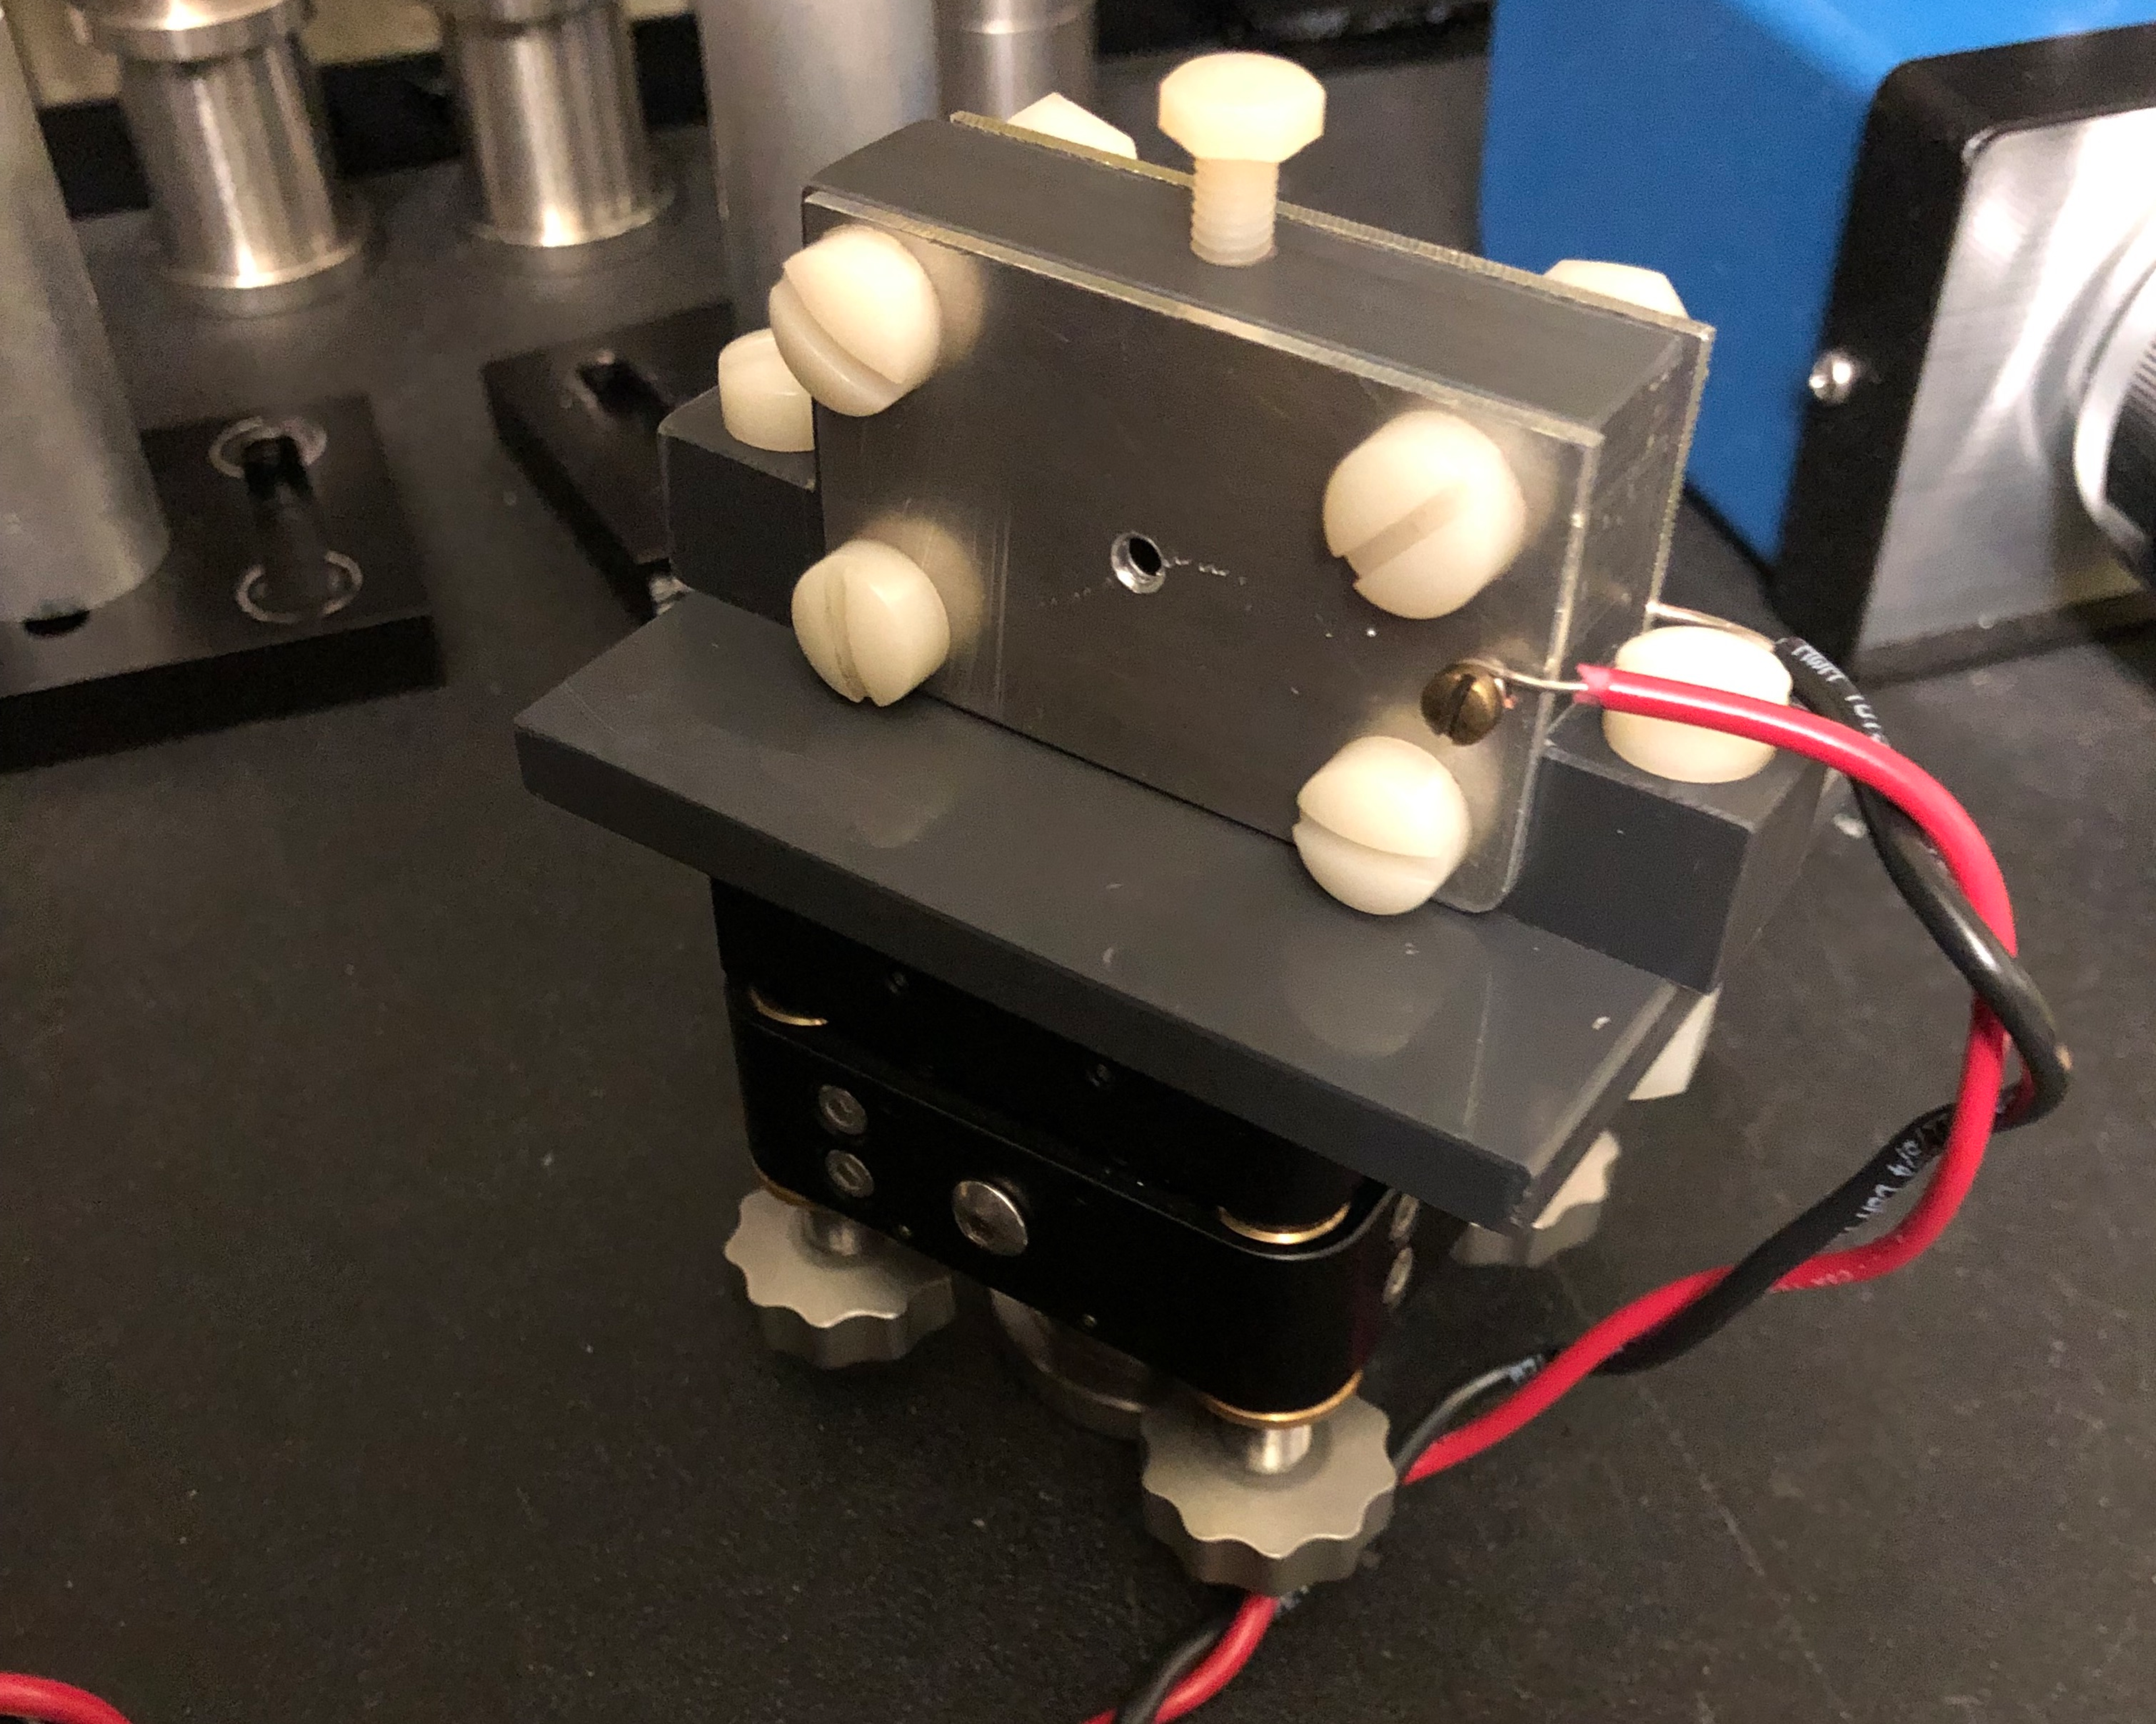
\includegraphics[width=.5\textwidth]{figs/ALGAAS/assemblies/assembly2/assembly2_PVC.pdf}
%		\phantomcaption\label{A2_PVC}
%		\includegraphics[width=.5\textwidth]{figs/ALGAAS/assemblies/assembly2/assembly2_PVC.pdf}
%		\phantomcaption\label{A2_PVC}
%    	\end{subcaptiongroup}
%    \caption{An iteration of assembly 2 comprised of a PVC mount with two rectangular (1.1"X2") plates with a central aperture of 3mm}
%    \label{fig:assembly2}
%\end{figure}

\begin{figure}[H]
    \includegraphics[width=\textwidth]{figs/ALGAAS/results_figs/assembly2/2_0_compare_1_1.pdf} 
    \caption{Assembly 2.0 transfer function measurements compared to Assembly 1.1, Measurements were taken from 1kHz up to 30kHz on using a Stanford Research 785 spectrum analyzer.}
    \label{fig:assembly2and1one}
\end{figure}


\begin{figure}[H]
    \includegraphics[width=\textwidth]{figs/ALGAAS/results_figs/assembly2/vary_da.pdf}
    \caption{The varied drive amplitudes input into the HVA to perform the following test}
    \label{fig:varyda}
\end{figure}

\begin{figure}[H]
    \includegraphics[width=\textwidth]{figs/ALGAAS/results_figs/assembly2/vv53.pdf} 
    \caption{Assembly 2.0 transfer function measurements with varied drive amplitudes indicated in ~\autoref{fig:varyda}.}
    \label{fig:vv53}
\end{figure}


\begin{figure}[H]
    \includegraphics[width=\textwidth]{figs/ALGAAS/results_figs/assembly2/vary_daao.pdf}
    \caption{The varied drive amplitudes and offsets input into the HVA to perform the following test}
    \label{fig:varydaao}
\end{figure}

\begin{figure}[H]
    \includegraphics[width=\textwidth]{figs/ALGAAS/results_figs/assembly2/vvao517.pdf} 
    \caption{Assembly 2.0 transfer function measurements with varied drive amplitudes and offsets indicated in ~\autoref{fig:varydaao}.}
    \label{fig:vvao517}
\end{figure}


\newpage

\subsection{Assembly 3 [MACOR] (blueprint)}
\subsubsection*{Model Params}
\begin{center}
\begin{tabular}{ |c|c|c|c|c|c| } 
\hline
$\mathrm{r}_{ap}$ [m] &  $\mathrm{t}_{cap}$ [m] & $\mathrm{r}_{el}$ [m] & $\mathrm{t}_{el}$ [m] & $\mathrm{r}_{opt}$ [m] & $\mathrm{t}_{opt}$ [m] \\
\hline
1.5e-3 & 6.94e-3 & 15.75e-3 & 9.66e-3 & 12.7e-3 & 6.35e-3 \\ 
\hline
\end{tabular}
\end{center}

\subsubsection*{Electrodes}
\begin{figure}[H]
  \centering
  \includegraphics[width=\textwidth]{figs/ALGAAS/assemblies/assembly3/electrode_3.pdf}
  \caption{Technical drawing of thick disk electrode plates made of copper.}
\end{figure}

\subsubsection*{Mount 3.0}

\begin{figure}[H]
\includegraphics[width=\textwidth]{figs/ALGAAS/assemblies/assembly3/MACOR_mount.pdf}
\caption{MACOR mount design constucted in Shapr3D}
\label{fig:macormountdesign}
\end{figure}

%\mbox{}
%\vfil

\newpage
\section{LaplacE code}

\subsection{laplace.py}
\begin{spacing}{1}
\begin{lstlisting}[frame=single, language=Python]
import numpy as np
import matplotlib.pyplot as plt
import h5py
from scipy.sparse import lil_matrix
from scipy.sparse import spdiags
import torch


# Computes Laplace's equation in cartesian and cylindrical coordinates
# For some related detailed documentation: Numerical recipies (3rd edition) 
  (Chapter 20 [Partial Differential Equations])


## Initialize fields

def init_coords(pdict):
    """ 
    Looks at params file to start implementing coordinate choices for simulation
    """
    if pdict['coords'] == 'cylindrical':
        if pdict['torch']:
            i_rho = torch.arange(pdict['origin'][0],pdict['N'][0])
            i_z = torch.arange(pdict['origin'][1],pdict['N'][1])
            rho_ = i_rho*torch.tensor(pdict['res'][0])
            z_ = i_z*torch.tensor(pdict['res'][1])
            rho, z = torch.meshgrid(rho_, z_, indexing='ij')
            invrho_ = 1/rho_
            invrho_[0] = 0
            invrho, z0 = torch.meshgrid(invrho_, z_, indexing='ij')
            
        else:
            i_rho = np.arange(pdict['origin'][0],pdict['N'][0])
            i_z  = np.arange(pdict['origin'][1],pdict['N'][1])                                          
            rho_ = i_rho*pdict['res'][0]google
            z_ = i_z*pdict['res'][1]
            rho = (rho_ * np.ones((pdict['N'][0],1)))
            rho = rho.reshape(pdict['N'][0]*pdict['N'][1],1)
            z  = (np.ones((pdict['N'][1],1)) * z_).T
            z = z.reshape(pdict['N'][0]*pdict['N'][1],1)
            invrho = 1/rho
            invrho[rho==0] = 0                                   # addresses inf elements
            
        coord_dict = {
            'coords' : {
                'rho' : rho, #np.round(rho,abs(int(np.log10(pdict['res'][0])))),
                'z' : z, #np.round(z,abs(int(np.log10(pdict['res'][0])))),
                'invrho' : invrho}, #np.round(invrho,abs(int(np.log10(pdict['res'][0]))))},
            'indices' : {
                'rho' : i_rho,
                'z' : i_z}
            }
        
    #elif pdict['coords'] == 'cartesian': 
    
    return coord_dict
    

def indx(icoord1, icoord2, N):
    """
    formalized lambda function reshaping potential (vectorizing V):
    indx = lambda i_rho, i_z : np.int32(i_rho + i_z*(N))
    """
    return np.int32(icoord1 + icoord2*N)


def idx_match(vec,N,step):
    """
    Acquire nearest matching ind(ex/ices) for queried location(s) in potential map
    """
    idx = np.int32(np.round(vec/step, decimals=0))
    idx = 1 if idx<1 else N if idx>N else idx
    return idx


def init_V(N):
    """
    Initialize (square) potential map
    """
    return np.zeros((N**2,1))
    

def build_lambd(i1, i2, N):
    """
    Constructs a matrix for a lambda function, which operates on all available indices in the simulation.
    Preallocates memory so that the indx function doesn't need to be used twice (reducing computations).
    """
    LAMBD = np.array([indx(i, i2, N) for i in i1])
    
    return LAMBD
        
    

def bc_set(pdict, BC, N, V):
    """
    Establishes simulation boundary conditions
    """
    #global R, d, step, idx, V, rho, z, bc0set
    
    #Plate bcs
    if pdict['coords'] == 'cylindrical':
        
        #Setting up the edge boundaries (for faster convergence)  
        if not bc0set:
            rho0 = False
            rhoend = np.interp(np.arange(0,N), np.array([0,N-1]),np.array([pdict['back_plate']['voltage'],pdict['front_plate']['voltage']])).reshape(N,1)
            z0 = pdict['back_plate']['voltage']
            zend = pdict['front_plate']['voltage']
            edge_vals =np.array(rho0, rhoend, z0, zend)
            V = bc_edge(pdict, edge_vals, V)
            bc0set = True
            
            
        #Set potentials
        for i in range(BC['cont']):
            V = set_pot(V,BC[i]['coords'],BC[i]['values'],LAMBD)
        
        # exponential boundary conditions
        V0 = 0
        R0 = 1
        V[idx(np.arange(0,N),N-1)] = V0  + np.exp(-step/R0)*(V[idx(np.arange(0,N), N-2)]-V0)
        V[idx(np.arange(0,N),0)] = V0 + np.exp(-step/R0)*(V[idx(np.arange(0,N),1)]-V0)
        V[idx(N-1,np.arange(0,N))]= V0 + np.exp(-step/R0)*(V[idx(N-2, np.arange(0,N))]-V0) 
                 
    return V
                 

                 

# Constructing the operator(s)
    
def build_lap(pdict, LAMBD, i_rho):
    """
    constructs first order structure of the laplace operator
    """
    if pdict['coords'] == 'cylindrical':
        
        op_shape = (pdict['N'][0]**2, pdict['N'][1]**2)
        
        if pdict['torch'] == True:
            idx_1 = LAMBD[0,1:-1]
            idx_2 = LAMBD[1,1:-1]
            idx_3 = LAMBD[0,:-2]
            idx_4 = LAMBD[0,2:]
            size_ = (pdict['N'][0]-2)**2
            idx_5 = LAMBD[1:-1,1:-1].reshape(size_)
            idx_6 = LAMBD[1:-1,:-2].reshape(size_)
            idx_7 = LAMBD[1:-1,2:].reshape(size_)
            idx_8 = LAMBD[:-2,1:-1].reshape(size_)
            idx_9 = LAMBD[2:,1:-1].reshape(size_)
            ones_1 = np.ones(idx_1.shape)
            ones_2 = np.ones(idx_5.shape)
            const_ = (np.ones((1,i_rho[1:-1].shape[0])).T*(((1/2)/(i_rho[1:-1])))).reshape(size_)
            lap1 = torch.sparse_coo_tensor(np.array([idx_1, idx_1]), -6*ones_1, op_shape, dtype=torch.float32)
            lap2 = torch.sparse_coo_tensor(np.array([idx_1, idx_2]), 4*ones_1, op_shape, dtype=torch.float32)
            lap3 = torch.sparse_coo_tensor(np.array([idx_1, idx_3]), ones_1, op_shape, dtype=torch.float32)
            lap4 = torch.sparse_coo_tensor(np.array([idx_1, idx_4]), ones_1, op_shape, dtype=torch.float32)
            lap5 = torch.sparse_coo_tensor(np.array([idx_5, idx_5]), -4*ones_2, op_shape, dtype=torch.float32)
            lap6 = torch.sparse_coo_tensor(np.array([idx_5, idx_6]), ones_2, op_shape, dtype=torch.float32)
            lap7 = torch.sparse_coo_tensor(np.array([idx_5, idx_7]), ones_2, op_shape, dtype=torch.float32)
            lap8 = torch.sparse_coo_tensor(np.array([idx_5, idx_8]), 1 - const_, op_shape, dtype=torch.float32)
            lap9 = torch.sparse_coo_tensor(np.array([idx_5, idx_9]), 1 + const_, op_shape, dtype=torch.float32)
            lap_ = lap1 + lap2 + lap3 + lap4 + lap5 + lap6 + lap7 + lap8 + lap9
            lap = lap_/(pdict['res'][0]**2)  
        else:
            lap = lil_matrix(op_shape,dtype=pdict['bitres'])
            lap[LAMBD[0,1:-1], LAMBD[0,1:-1]] = -6
            lap[LAMBD[0,1:-1], LAMBD[1,1:-1]] = 4
            lap[LAMBD[0,1:-1], LAMBD[0,:-2]] = 1
            lap[LAMBD[0,1:-1], LAMBD[0,2:]] = 1
            lap[LAMBD[1:-1,1:-1], LAMBD[1:-1,1:-1]] = -4
            lap[LAMBD[1:-1,1:-1], LAMBD[1:-1,:-2]] = 1
            lap[LAMBD[1:-1,1:-1], LAMBD[1:-1,2:]] = 1
            lap[LAMBD[1:-1,1:-1], LAMBD[:-2,1:-1]]= 1 - ((1/2)/(i_rho[1:-1]))
            lap[LAMBD[1:-1,1:-1], LAMBD[2:,1:-1]]= 1 + ((1/2)/(i_rho[1:-1]))
            lap = lap/(pdict['res'][0]**2)
        
    #elif pdict['coords'] == 'cartesian':
        
    return lap

def build_grad(pdict, LAMBD):
    """
    Gradient operators 
    """
    if pdict['coords'] == 'cylindrical': 
        if pdict['torch'] == True:
            
            idx1 = LAMBD[1:-1,:]
            idx2 = LAMBD[:-2,:]
            idx3 = LAMBD[2:,:]
            idx4 = LAMBD[:,1:-1]
            idx5 = LAMBD[:,:-2]
            idx6 = LAMBD[:,2:]
            
            gradrho1 = torch.sparse_coo_tensor(np.array([idx1, idx2]), -1/2, op_shape, dtype=pdict['bitres'])
            gradrho2 = torch.sparse_coo_tensor(np.array([idx1, idx3]), -1/2, op_shape, dtype=pdict['bitres'])
            GRADrho = (gradrho1+gradrho2)/pdict['res'][0]
            
            gradrhopos1 = torch.sparse_coo_tensor(np.array([idx1, idx1]), -1, op_shape, dtype=pdict['bitres'])
            gradrhopos2 = torch.sparse_coo_tensor(np.array([idx1, idx3]), -1, op_shape, dtype=pdict['bitres'])
            GRADrhopos = (gradrhopos1+gradrhopos2)/pdict['res'][0]
            
            gradrhoneg1 = torch.sparse_coo_tensor(np.array([idx1, idx2]), -1, op_shape, dtype=pdict['bitres'])
            gradrhoneg2 = torch.sparse_coo_tensor(np.array([idx1, idx1]), -1, op_shape, dtype=pdict['bitres'])
            GRADrhoneg = (gradrhoneg1+gradrhoneg2)/pdict['res'][0]
            
            gradz1 = torch.sparse_coo_tensor(np.array([idx4, idx5]), -1/2, op_shape, dtype=pdict['bitres'])
            gradz2 = torch.sparse_coo_tensor(np.array([idx4, idx6]), -1/2, op_shape, dtype=pdict['bitres'])
            GRADz = (gradz1+gradz2)/pdict['res'][1]
            
            gradzpos1 = torch.sparse_coo_tensor(np.array([idx4, idx4]), -1, op_shape, dtype=pdict['bitres'])
            gradzpos2 = torch.sparse_coo_tensor(np.array([idx4, idx6]), 1, op_shape, dtype=pdict['bitres'])
            GRADzpos = (gradzpos1 + gradzpos2)/pdict['res'][1]
            
            gradzpos1 = torch.sparse_coo_tensor(np.array([idx4, idx5]), -1, op_shape, dtype=pdict['bitres'])
            gradzpos2 = torch.sparse_coo_tensor(np.array([idx4, idx4]), 1, op_shape, dtype=pdict['bitres'])
            GRADzneg = (gradzpos1 + gradzpos2)/pdict['res'][1]
            
        else:
            
            init_sparmat = lambda shape, res : lil_matrix(shape, dtype = res)
            
            op_shape = (pdict['N'][0]**2, pdict['N'][1]**2)
            
            GRADrho = init_sparmat(op_shape, pdict['bitres'])
            GRADrho[LAMBD[1:-1,:], LAMBD[:-2,:]] = -1/2
            GRADrho[LAMBD[1:-1,:], LAMBD[2:,:]]= 1/2
            GRADrho = GRADrho/pdict['res'][0]

            GRADrhopos = init_sparmat(op_shape, pdict['bitres'])
            GRADrhopos[LAMBD[1:-1,:], LAMBD[1:-1,:]] = -1
            GRADrhopos[LAMBD[1:-1,:], LAMBD[2:,:]]= 1
            GRADrhopos = GRADrhopos/pdict['res'][0]

            GRADrhoneg = init_sparmat(op_shape, pdict['bitres'])
            GRADrhoneg[LAMBD[1:-1,:], LAMBD[:-2,:]] = -1
            GRADrhoneg[LAMBD[1:-1,:], LAMBD[1:-1,:]]= 1
            GRADrhoneg = GRADrhoneg/pdict['res'][0]

            GRADz= init_sparmat(op_shape, pdict['bitres'])
            GRADz[LAMBD[:,1:-1], LAMBD[:,:-2]] = -1/2
            GRADz[LAMBD[:,1:-1], LAMBD[:,2:]]= 1/2
            GRADz = GRADz/pdict['res'][1]

            GRADzpos= init_sparmat(op_shape, pdict['bitres'])
            GRADzpos[LAMBD[:,1:-1], LAMBD[:,1:-1]] = -1
            GRADzpos[LAMBD[:,1:-1], LAMBD[:,2:]]= 1
            GRADzpos = GRADzpos/pdict['res'][1]

            GRADzneg= init_sparmat(op_shape, pdict['bitres'])
            GRADzneg[LAMBD[:,1:-1], LAMBD[:,:-2]] = -1
            GRADzneg[LAMBD[:,1:-1], LAMBD[:,1:-1]]= 1
            GRADzneg = GRADzneg/pdict['res'][1]
        
        
    return GRADrho, GRADrhopos, GRADrhoneg, GRADz, GRADzpos, GRADzneg


def build_disp(pdict, LAMBD):
    """
    Displacement operators
    """
    
    if pdict['coords'] == 'cylindrical':
        DISPrhopos = lil_matrix((pdict['N'][0]**2, pdict['N'][1]**2),dtype=pdict['bitres'])
        DISPrhopos[LAMBD[1:,:], LAMBD[:-1,:]] = 1

        DISPrhoneg = lil_matrix((pdict['N'][0]**2, pdict['N'][1]**2),dtype=pdict['bitres'])
        DISPrhoneg[LAMBD[:-1,:], LAMBD[1:,:]] = 1

        DISPzpos = lil_matrix((pdict['N'][0]**2, pdict['N'][1]**2),dtype=pdict['bitres'])
        DISPzpos[LAMBD[:,1:], LAMBD[:,:-1]] = 1

        DISPzneg = lil_matrix((pdict['N'][0]**2, pdict['N'][1]**2),dtype=pdict['bitres'])
        DISPzneg[LAMBD[:,:-1], LAMBD[:,1:]] = 1
        
    return DISPrhopos, DISPrhoneg, DISPzpos, DISPzneg
             
def build_LAP(pdict, coord_dict, lap, grad, disp, chi_e):
    """
    full laplace operator (dielectric considerations)
    """
    if pdict['coords'] == 'cylindrical':
        GRADrho = grad[0]
        GRADrhopos = grad[1]
        GRADrhoneg = grad[2]
        GRADz = grad[3]
        GRADzpos = grad[4]
        GRADzneg = grad[5]
        
        DISPrhopos = disp[0]
        DISPrhoneg = disp[1]
        DISPzpos = disp[2]
        DISPzneg = disp[3]
    
        chi_e_half = chi_e/2

        CHI1 = spdiags((1/(1+chi_e_half)).T,0, pdict['N'][0]*pdict['N'][1], pdict['N'][0]*pdict['N'][1], format='lil')
        CHI2 = spdiags((chi_e_half*coord_dict['coords']['invrho']).T,0, pdict['N'][0]*pdict['N'][1], pdict['N'][0]*pdict['N'][1], format='lil')
        DNEG = spdiags(DISPrhoneg.dot(chi_e_half).T,0, pdict['N'][0]*pdict['N'][1], pdict['N'][0]*pdict['N'][1], format='lil')
        DPOS = spdiags(DISPrhopos.dot(chi_e_half).T,0, pdict['N'][0]*pdict['N'][1], pdict['N'][0]*pdict['N'][1], format='lil')
        ZNEG = spdiags(DISPzneg.dot(chi_e_half).T,0, pdict['N'][0]*pdict['N'][1], pdict['N'][0]*pdict['N'][1], format='lil')
        ZPOS = spdiags(DISPzpos.dot(chi_e_half).T,0, pdict['N'][0]*pdict['N'][1], pdict['N'][0]*pdict['N'][1], format='lil')
        LAP = lap + CHI1.dot(CHI2.dot(GRADrho) + (DNEG.dot(GRADrhopos) - DPOS.dot(GRADrhoneg))/pdict['res'][0] + (ZNEG.dot(GRADzpos) - ZPOS.dot(GRADzneg))/pdict['res'][1]) 
        
    #elif pdict['coords'] == 'cartesian':
        
    return LAP



def anal_sol(pdict):
    z_p1 = pdict['front_plate']['zpos']
    z_p2 = pdict['back_plate']['zpos']
    d_plates = z_p1 - z_p2
    V_p1 = pdict['front_plate']['voltage']
    V_p2 = pdict['back_plate']['voltage']
    V_diff = V_p1 - V_p2
    d_opt = pdict['optic']['thickness']
    d_sub = pdict['optic']['sub_thickness']
    d_coat = pdict['optic']['coat_thickness']
    d_air = pdict['cap_params']['d_air']
    z_opt = pdict['optic']['z_com']
    p1_2_opt  = z_p1 - (d_opt/2.0) - z_opt
    opt_2_p2 = z_opt - (d_opt/2.0) - z_p2
    eps_air = pdict['cap_params']['air_eps']
    eps_sub = pdict['optic']['sub_eps']   
    eps_coat = pdict['optic']['coat_eps']
    CoA = pdict['cap_params']['cap_div_area']
    cap_ratio = CoA
    air_ratio = d_air/eps_air
    sub_ratio = d_sub/eps_sub
    coat_ratio = d_coat/eps_coat
    V_air = cap_ratio*air_ratio*V_diff
    V_coat = cap_ratio*coat_ratio*V_diff
    V_sub = cap_ratio*sub_ratio*V_diff
    

    #E_front = V_diff/(p1_2_opt + opt_2_p2 + (d_opt-d_coat)/eps_sub + d_coat/eps_coat)
    #E_sub = V_diff/((p1_2_opt + opt_2_p2 + d_coat/eps_coat)*eps_sub + (d_opt-d_coat))
    #E_coat = V_diff/( (p1_2_opt + opt_2_p2 + (d_opt-(d_coat))/eps_sub)*eps_coat + d_coat)
    #E_back = E_front
    z_anal = z_p2+np.array([0, opt_2_p2, (opt_2_p2 + d_sub), (opt_2_p2 + d_sub + d_coat), (opt_2_p2 + d_sub + d_coat + opt_2_p2)])
    V_anal = np.array([V_p2, V_p2 + V_air, V_p2 + V_air + V_sub, V_p2 + V_air + V_sub + V_coat, V_p1])
    anal_dict = {
        'V_anal' : lambda z: np.interp(z, z_anal, V_anal)
        }
    return anal_dict


def pltxsect(loc_params, coord_dict, V): 
    if loc_params['cross_section_coord'] == 'z':
        rho_ = coord_dict['coords']['rho'] == np.around(loc_params['rho'], int(abs(np.log10(coord_dict['coords']['rho'][1]))))
        z_ = np.logical_and(coord_dict['coords']['z']<=loc_params['z1_bound'], coord_dict['coords']['z']>=loc_params['z2_bound'])
        plt.plot(coord_dict['coords']['z'][np.logical_and(rho_,z_)],V[np.logical_and(rho_, z_)])
    if loc_params['cross_section_coord'] == 'rho':
        z_ = coord_dict['coords']['z'] == np.around(loc_params['z'], int(abs(np.log10(coord_dict['coords']['z'][1]))))
        rho_ = np.logical_and(coord_dict['coords']['rho']<=loc_params['rho2_bound'], coord_dict['coords']['rho']>=loc_params['rho1_bound'])
        plt.plot(coord_dict['coords']['rho'][np.logical_and(rho_,z_)],V[np.logical_and(rho_, z_)])
\end{lstlisting}
\end{spacing}


\subsection{set\_params.py}
\begin{spacing}{1.2}
\begin{lstlisting}[frame=single, language=Python]
import numpy as np
## Setting parameters
pdict ={
    'coords' : 'cylindrical'             ,                        # coordinate system chosen for simulation box
    'assembly' : 1                       ,                        # Establish plate geometry / location and voltage based on assembly 
    'origin' : np.array([0,0])           ,                        # Origin of the simulation space / map
    'size' : np.array([.04, .04])        ,                        # Size of simulation box [m] 
    'res' : np.array([1,1])*1e-6         ,                        # relative resolution [coord1, coord2]
    'iters' : 100000                     ,                        # total number of time iterations
    'iter_step' : 0.1                    ,                        # time step
    'expbc' : False                      ,                        # Exponential boundary conditions?
    'bitres' : 'float32'                 ,                        # matrix element data type ('float32' vs 'float64')
    'in2m' : .0254                       ,                        # frequently used conversion
    'torch': True
}
    
pdict['res_exp'] = np.abs(np.log10(pdict['res'])).astype('int')
pdict['aspect'] = pdict['size'][0] == pdict['size'][1]
pdict['N'] = (pdict['size']*(1/pdict['res']) + 1).astype('int')   
    # number of points sampled 1 dimension of simulation box

# Sample parameters
pdict['optic'] =  {
        "diam" : 1.0*pdict['in2m'],
        "thickness" : .25*pdict['in2m'], 
        "z_com" : pdict['size'][1]/2,
        "sub_eps" : 3.82,                                        # dielectric constant for substrate (fused silica)
        "coat_eps" : 13.436,                                     # dielectric constant for coating material (AlGaAs / GaAs)
        "coat_thickness" : 9.5e-6     
}

pdict['optic']['sub_thickness'] = pdict['optic']['thickness'] - pdict['optic']['coat_thickness']

# CHOOSING ASSEMBLY CONFIGURATION
    # Parameters established to characterize the assembly configurations:
        # Front and back plate dimensions (usually disk diameters)
        # Central aperture diameter
        # Plate positioning along the beam axis with respect to simulation size center
        # Maximum AC voltage sent on respective plates

maxhva_settings = {
        "SVR350" : 210,                                         # [Vpk]
        "TREK2220" : 220,                                       # [Vpk]
        "TREK5/80" : 1000,                                      # [Vpk]
        "TREK10/10B-HS" : 1040                                  # [Vpk]
} 

if pdict['assembly'] == 0 or pdict['assembly'] == 1:
    # Setting front and back plate params (including spacing between
    # 	them and voltage on respective plates)
    # This assembly has an assortment of 3d printed spacer components
    pdict['HVA'] = "SVR350"
    pdict['mount_zdims'] = {
        "back_ring" : 1e-3,                                    # +/- 2e-4 [m]
        "sample_holder" : 9e-3,                                # +/- 2e-4 [m]
        "electrode_brace": 3e-3 ,                              # +/- 2e-4 [m]
        "electrode_backing": 2e-3                              # +/- 2e-4 [m]
    }
    pdict['front_plate'] = {
        "diam" : 3* pdict['in2m'],                             # diameter of plate [m]
        "hole_diam" : 3e-3,                                    # aperture diameter [m]
        "thickness" : 1.5e-3,
        "zpos" : pdict['size'][1]/2 + pdict['mount_zdims']["sample_holder"]/2,
	    # location of plate surface (com) [m]
        "voltage" : maxhva_settings[pdict['HVA']]                       # Voltage on front plate [V]
    }
    pdict['back_plate'] = {
        "diam" : 3*pdict['in2m'], 
        "hole_diam" : 3e-3,
        "thickness" : 1.5e-3, 
        "zpos" : pdict['size'][1]/2 - pdict['mount_zdims']["sample_holder"]/2,
        "voltage" : - maxhva_settings[pdict['HVA']]
    } 
elif pdict['assembly'] == 2 : 
    # Overall thickness was approximately .5 inches with a 
    #	.125 inch lip on one end and .125 gap on the other end of sample.
    # Once the sample was dropped into the mount with the 
    #	surface hugging the PVC lip, it was held down with a nylon set screw 
	(with a rubberized tip.)
    # This plate used is an aluminum rectangular plate 
    #	(will incorporate cartesian coordinates into program soon.)
    pdict['HVA'] = "SVR350"
    pdict['mount_zdims'] = {
        "sample_holder" : .5*pdict['in2m']
    }
    if pdict['coords'] == 'cartesian':
        pdict['front_plate'] = {
            "diam" : 0.02794,                                 # diameter of plate [m]
            "hole_diam" : 3e-3,                               # aperture diameter [m]
            "thickness" : 1.27e-3, 
            "zpos" : pdict['size'][1]/2 + pdict['mount_zdims']["sample_holder"]/2,    
		# location of plate surface (com) [m]
            "voltage" : maxhva_settings[pdict['HVA']]/2
		# Voltage on front plate [V] (MAX value for associated HVA)
        }
        pdict['back_plate'] = {
            "diam" : 0.02794,
            "hole_diam" : 3e-3,
            "thickness" : 1.27e-3, 
            "zpos" : pdict['size'][1]/2 - pdict['mount_zdims']["sample_holder"]/2,
            "voltage" : - maxhva_settings[pdict['HVA']]/2
        }
    elif pdict['coords'] == 'cylindrical':
        pdict['front_plate'] = {
            "diam" : 0.02794,                                 # diameter of plate [m]
            "hole_diam" : 3e-3,                               # aperture diameter [m]
            "thickness" : 1.27e-3, 
            "zpos" : pdict['size'][1]/2 + pdict['mount_zdims']["sample_holder"]/2,    
		# location of plate surface (com) [m]
            "voltage" : maxhva_settings[pdict['HVA']]/2                                  # Voltage on front plate [V]
        }
        pdict['back_plate'] = {
            "diam" : 0.02794,
            "hole_diam" : 3e-3,
            "thickness" : 1.27e-3, 
            "zpos" : pdict['size'][1]/2 - pdict['mount_zdims']["sample_holder"]/2,
            "voltage" : maxhva_settings[pdict['HVA']]/2  
        }
        
elif pdict['assembly'] == 3 :
    #Set front and back plate params
    pdict['HVA'] =  "TREK10/10B-HS"
    pdict['mount_zdims'] = {
        "total_zthickness" : 25.94e-3 ,                         # holds both sample and both electrodes [m]
        "sample_holder" : 6.94e-3                              # width of lip that separates sample from electrodes [m] 
    }
    pdict['front_plate'] = {
        "diam" : 31.5e-3,                                       # diameter of plate [m]
        "hole_diam" : 3e-3,                                  # aperture diameter [m]
        "thickness" : 9.66e-3, 
        "zpos" : pdict['size'][1]/2 + (pdict['mount_zdims']["sample_holder"]/2),      
	    # location of plate surface (com) [m]
        "voltage" : maxhva_settings[pdict['HVA']]/2                                     
	    # Voltage on front plate [V]
    }
    pdict['back_plate'] = {
        "diam" : 31.5e-3,
        "hole_diam" : 3e-3,
        "thickness" : 9.66e-3, 
        "zpos" : pdict['size'][1]/2 - (pdict['mount_zdims']["sample_holder"]/2),
        "voltage" : -maxhva_settings[pdict['HVA']]/2
    }
    
elif pdict['assembly'] == 4 :
    #Set front and back plate params
    pdict['mount_zdims'] = {
        "total_zthickness" : 25.94e-3 ,                         # holds both sample and both electrodes [m]
        "sample_holder" : 6.94e-3                              # width of lip that separates sample from electrodes [m] 
    }
    pdict['front_plate'] = {
        "diam" : 31.5e-3,                                       # diameter of plate [m]
        "hole_diam" : 3e-3,                                  # aperture diameter [m]
        "thickness" : 9.66e-3, 
        "zpos" : pdict['size'][1]/2 + (pdict['mount_zdims']["sample_holder"]/2),      
	    # location of plate surface (com) [m]
        "voltage" :  maxhva_settings[pdict['HVA']]/2                                      # Voltage on front plate [V]
    }
    pdict['back_plate'] = {
        "diam" : 31.5e-3,
        "hole_diam" : 3e-3,
        "thickness" : 9.66e-3, 
        "zpos" : pdict['size'][1]/2 - (pdict['mount_zdims']["sample_holder"]/2),
        "voltage" : - maxhva_settings[pdict['HVA']]/2 
    }
    
pdict['cap_params'] = {
        "area" : np.pi*((pdict['front_plate']['diam']/2.0)**2), 
        "d_air": (pdict['mount_zdims']['sample_holder']-pdict['optic']['thickness'])/2.0, 
        "air_eps" : 1.0006
    }

pdict['cap_params']['cap_div_area'] = (pdict['optic']['sub_eps']*pdict['optic']['coat_eps']*
    pdict['cap_params']['air_eps'])/((2.0*pdict['optic']['sub_eps']*pdict['optic']['coat_eps']*
    pdict['cap_params']['d_air']) + (pdict['optic']['sub_eps']*pdict['cap_params']['air_eps']*
    pdict['optic']['coat_thickness']) + (pdict['optic']['coat_eps']*
    pdict['cap_params']['air_eps']*(pdict ['optic']['sub_thickness'])))
pdict['cap_params']['capacitance'] = pdict['cap_params']['cap_div_area']*
    pdict['cap_params']['area']

# system location params / metadata
pdict['loc_params'] = {
    'center of optic' : {
        'cross_section_coord' : 'z',
        'rho' : 0,
        'z1_bound' : pdict['front_plate']['zpos'],
        'z2_bound' : pdict['back_plate']['zpos']
    },
    'edge of hole' : {
        'cross_section_coord' : 'z',
        'rho' : pdict['front_plate']['hole_diam'],
        'z1_bound' : pdict['front_plate']['zpos'],
        'z2_bound' : pdict['back_plate']['zpos']
    },
    'edge of optic' : {
        'cross_section_coord' : 'z',
        'rho' : pdict['optic']['diam'] /2,
        'z1_bound' : pdict['front_plate']['zpos'],
        'z2_bound' : pdict['back_plate']['zpos']
    },
    'edge of plate' : {
        'cross_section_coord' : 'z',
        'rho' : pdict['front_plate']['diam']/2,
        'z1_bound' : pdict['front_plate']['zpos'],
        'z2_bound' : pdict['back_plate']['zpos']
    },
    'halfway out on optic' : {
        'cross_section_coord' : 'z',
        'rho' : pdict['optic']['diam']/4,
        'z1_bound' : pdict['front_plate']['zpos'],
        'z2_bound' : pdict['back_plate']['zpos']
    },
    'front of plate' : {
        'cross_section_coord' : 'rho',
        'rho1_bound' : 0,
        'rho2_bound' : pdict['size'],
        'z' : pdict['back_plate']['zpos']
    },
    'front of optic' : {
        'cross_section_coord' : 'rho',
        'rho1_bound' : 0,
        'rho2_bound' : pdict['size'],
        'z' : pdict['optic']['z_com'] + pdict['optic']['thickness']/2
    },
    'middle of optic' : {
        'cross_section_coord' : 'rho',
        'rho1_bound' : 0,
        'rho2_bound' : pdict['size'],
        'z' : pdict['optic']['z_com']
    },
    'back of optic' : {
        'cross_section_coord' : 'rho',
        'rho1_bound' : 0,
        'rho2_bound' : pdict['size'],
        'z' : pdict['optic']['z_com'] - pdict['optic']['thickness']/2
    },
    'back plate' : {
        'cross_section_coord' : 'rho',
        'rho1_bound' : 0,
        'rho2_bound' : pdict['size'],
        'z' : pdict['back_plate']['zpos']
    }
}
\end{lstlisting}
\end{spacing}


\subsection{run.py}
The numerical recipe is written up fabulously in Chapter 20  of \cite{Press:2007} for any inquiring minds.
\begin{lstlisting}[frame=single, language=Python]
import set_params
import laplace
import matplotlib.pyplot as plt
import numpy as np
plt.style.use('stylelib/surftex')
#fig_exp_dirama = "../../../../dissertation/figs/ALGAAS/"
from matplotlib import cm
from matplotlib import rcParams
import time
import torch
\end{lstlisting}

\hypertarget{params-import}{%
\subsection{Params Import}\label{params-import}}

\begin{lstlisting}[frame=single, language=Python]
pdict = set_params.pdict
pdict
\end{lstlisting}

\begin{lstlisting}[frame=single, language=Python]
{'coords': 'cylindrical',
 'assembly': 1,
 'origin': array([0, 0]),
 'size': array([0.04, 0.04]),
 'res': array([0.0001, 0.0001]),
 'iters': 100000,
 'iter_step': 0.1,
 'expbc': False,
 'bitres': 'float32',
 'in2m': 0.0254,
 'res_exp': array([4, 4]),
 'aspect': True,
 'N': array([401, 401]),
 'optic': {'diam': 0.0254,
  'thickness': 0.00635,
  'z_com': 0.02,
  'sub_eps': 3.82,
  'coat_eps': 13.436,
  'coat_thickness': 9.5e-06,
  'sub_thickness': 0.0063405},
 'HVA': 'SVR350',
 'mount_zdims': {'back_ring': 0.001,
  'sample_holder': 0.009,
  'electrode_brace': 0.003,
  'electrode_backing': 0.002},
 'front_plate': {'diam': 0.07619999999999999,
  'hole_diam': 0.003,
  'thickness': 0.0015,
  'zpos': 0.0245,
  'voltage': 210},
 'back_plate': {'diam': 0.07619999999999999,
  'hole_diam': 0.003,
  'thickness': 0.0015,
  'zpos': 0.0155,
  'voltage': -210},
 'cap_params': {'area': 0.004560367311877479,
  'd_air': 0.0013249999999999998,
  'air_eps': 1.0006,
  'cap_div_area': 232.07592015102685,
  'capacitance': 1.0583514401306306},
 'loc_params': {'center of optic': {'cross_section_coord': 'z',
   'rho': 0,
   'z1_bound': 0.0245,
   'z2_bound': 0.0155},
  'edge of hole': {'cross_section_coord': 'z',
   'rho': 0.003,
   'z1_bound': 0.0245,
   'z2_bound': 0.0155},
  'edge of optic': {'cross_section_coord': 'z',
   'rho': 0.0127,
   'z1_bound': 0.0245,
   'z2_bound': 0.0155},
  'edge of plate': {'cross_section_coord': 'z',
   'rho': 0.038099999999999995,
   'z1_bound': 0.0245,
   'z2_bound': 0.0155},
  'halfway out on optic': {'cross_section_coord': 'z',
   'rho': 0.00635,
   'z1_bound': 0.0245,
   'z2_bound': 0.0155},
  'front of plate': {'cross_section_coord': 'rho',
   'rho1_bound': 0,
   'rho2_bound': array([0.04, 0.04]),
   'z': 0.0155},
  'front of optic': {'cross_section_coord': 'rho',
   'rho1_bound': 0,
   'rho2_bound': array([0.04, 0.04]),
   'z': 0.023175},
  'middle of optic': {'cross_section_coord': 'rho',
   'rho1_bound': 0,
   'rho2_bound': array([0.04, 0.04]),
   'z': 0.02},
  'back of optic': {'cross_section_coord': 'rho',
   'rho1_bound': 0,
   'rho2_bound': array([0.04, 0.04]),
   'z': 0.016825},
  'back plate': {'cross_section_coord': 'rho',
   'rho1_bound': 0,
   'rho2_bound': array([0.04, 0.04]),
   'z': 0.0155}}}
\end{lstlisting}

\hypertarget{initializing-coordinates-simulation-space}{%
\subsection{Initializing coordinates / simulation
space}\label{initializing-coordinates-simulation-space}}

\begin{lstlisting}[frame=single, language=Python]
# initialize coordinates
coord_dict = laplace.init_coords(pdict) 

# Imposing a square simulation space
N = pdict['N'][0]

# coord vecs
rho = coord_dict['coords']['rho']
z = coord_dict['coords']['z']
inv_rho = coord_dict['coords']['invrho']

#indices 
irho = coord_dict['indices']['rho']
iz = coord_dict['indices']['z']
\end{lstlisting}

\begin{lstlisting}[frame=single, language=Python]
/Users/dancvan/Documents/git/cylaplace/laplace.py:27: RuntimeWarning: divide by zero encountered in true_divide
  invrho = 1/rho
\end{lstlisting}

\hypertarget{potential-map-initialization-v-with-dielectric-tensor-initialization-chi_e}{%
\section{Potential map initialization (V) with Dielectric tensor
initialization
(chi\_e)}\label{potential-map-initialization-v-with-dielectric-tensor-initialization-chi_e}}

\begin{lstlisting}[frame=single, language=Python]
fV = laplace.anal_sol(pdict)
\end{lstlisting}

\begin{lstlisting}[frame=single, language=Python]
plt.plot(coord_dict['indices']['z']*1e-4,fV['V_anal'](coord_dict['indices']['z']*1e-4))
\end{lstlisting}

\begin{lstlisting}[frame=single, language=Python]
# intialize potential map, electric susceptibility, and LAMBD operator
V = laplace.init_V(N)
chi_e = laplace.init_V(N)
chi_e_sub = pdict['optic']['sub_eps']-1
chi_e_coat = pdict['optic']['coat_eps']-1
LAMBD = laplace.build_lambd(irho, iz, N)
\end{lstlisting}

\begin{lstlisting}[frame=single, language=Python]
# Translating (Dirichlet) boundary conditions to sim 

# Initial value 

## (For faster convergence) setting edge values

### Edge locations
r_max = (rho == max(rho))
r_min = (rho == min(rho))
z_max = (z == max(z))
z_min = (z == min(z))

# Boundary values 

## Plate potentials
fp = 'front_plate'
bp = 'back_plate'
loc_fp = np.logical_and(np.logical_and(rho>=pdict[fp]['hole_diam']/2,rho<=pdict[fp]['diam']/2),z == pdict[fp]['zpos'])
loc_bp = np.logical_and(np.logical_and(rho>=pdict[bp]['hole_diam']/2,rho<=pdict[bp]['diam']/2),z == pdict[bp]['zpos'])
#bc_fp = laplace.BC_dict([[pdict[fp]['hole_diam']/2, pdict[fp]['diam']/2], pdict[fp]['zpos']],pdict[fp]['voltage'],fp, LAMBD)
#bc_bp = laplace.BC_dict([[pdict[bp]['hole_diam']/2, pdict[bp]['diam']/2], pdict[bp]['zpos']],pdict[fp]['voltage'],bp, LAMBD)

# Exponential boundary conditions
exp_rend  = rho==(max(rho)-pdict['res'][0])

exp_z0 = z==(min(z)+pdict['res'][1])

exp_zend = z==(max(z)-pdict['res'][1])

# Setting sample dielectric
loc_sub = np.logical_and(np.abs(z - pdict['optic']['z_com']) < np.round((pdict['optic']['thickness']/2),pdict['res_exp'][1]), (rho<np.round((pdict['optic']['diam']/2),pdict['res_exp'][0])))
loc_coat1 = np.logical_and((z==np.round(pdict['loc_params']['front of optic']['z'],pdict['res_exp'][1])), (rho < np.round((pdict['optic']['diam']/2), pdict['res_exp'][0])))
loc_coat2 = np.logical_and((z==np.round((pdict['loc_params']['front of optic']['z']-pdict['res'][1]),pdict['res_exp'][1])), (rho < (np.round(pdict['optic']['diam']/2, pdict['res_exp'][0]))))
\end{lstlisting}

\begin{lstlisting}[frame=single, language=Python]
## Initialize BCs

#### Set susceptibility
chi_e[loc_sub] = chi_e_sub
chi_e[loc_coat1] = chi_e_coat
chi_e[loc_coat2] = chi_e_coat

## Electro-static conditions

### Electrode plates
V[loc_fp] = pdict[fp]['voltage']
V[loc_bp] = pdict[bp]['voltage']

#### Boundary values

#### Edge for faster convergance
V[z_min] = pdict['back_plate']['voltage']
V[z_max] = pdict['front_plate']['voltage']
V[r_max] = np.interp(np.arange(0,pdict['N'][0]), np.array([0,pdict['N'][0]-1]), np.array([pdict['back_plate']['voltage'], pdict['front_plate']['voltage']]))

### Exponential (Dirichlet) boundary conditions
V_exp = lambda V_0, R_0, V , R : V_0 + np.exp(-R/R_0)*(V - V_0) 
V_char = 0
R_char = 1.0

#rho=rho_max
V[r_max] = V_exp(V_char, R_char, V[exp_rend], pdict['res'][0])
#z=z_min
V[z_min] = V_exp(V_char, R_char, V[exp_z0], pdict['res'][1])
#z=z_max
V[z_max] = V_exp(V_char, R_char, V[exp_zend], pdict['res'][1])
\end{lstlisting}

\begin{lstlisting}[frame=single, language=Python]
#### Build operators
lap = laplace.build_lap(pdict, LAMBD, irho)
grad = laplace.build_grad(pdict, LAMBD)
disp = laplace.build_disp(pdict, LAMBD)
LAP = laplace.build_LAP(pdict, coord_dict, lap, grad, disp, chi_e)
\end{lstlisting}

\begin{lstlisting}[frame=single, language=Python]
t = time.time() 
#### run sim
for itr in range(0, pdict['iters']):
    
    V = V + (pdict['res'][0]*pdict['res'][0]*pdict['iter_step']*LAP.dot(V))
    
    ## Re-applying exponential condition
    #rho=rho_max
    V[r_max] = V_exp(V_char, R_char, V[exp_rend], pdict['res'][0])
    #z=z_min
    V[z_min] = V_exp(V_char, R_char, V[exp_z0], pdict['res'][1])
    #z=z_max
    V[z_max] = V_exp(V_char, R_char, V[exp_zend], pdict['res'][1])
    
    ### Re-apply Electro-static condition
    V[loc_fp] = pdict[fp]['voltage']
    V[loc_bp] = pdict[bp]['voltage']
elapsed = time.time() - t
print(elapsed)
\end{lstlisting}

\begin{lstlisting}
84.81229615211487
\end{lstlisting}

\begin{lstlisting}[frame=single, language=Python]
fig = plt.figure(figsize = (18.5,21))
ax = plt.axes(projection='3d') 
surf = ax.plot_surface(rho.reshape(N,N), z.reshape(N,N),V.reshape(N,N),rstride=1,cstride=1,cmap=cm.inferno,alpha=1,linewidth=10,rasterized=True)
fig.tight_layout()
ax.view_init(20,210)
ax.set_xlabel('r [m]')
ax.set_ylabel('z [m]')
ax.set_zlabel('[V]')
fig.colorbar(surf, shrink=0.4, aspect=20, pad=-0.025)
axes_width = fig.get_size_inches()[1]*(fig.subplotpars.right-fig.subplotpars.left)
right =1.095
left =-.15
fig.subplots_adjust(left=left,right=right) 
fig.set_size_inches((fig.get_size_inches()[0],axes_width/(right-left)))
ax.tick_params(axis='both', pad=15)
axes_height = fig.get_size_inches()[1]*(fig.subplotpars.top-fig.subplotpars.bottom)
top = 1.15
bottom=-.09
fig.subplots_adjust(top=top,bottom=bottom)             
fig.set_size_inches((fig.get_size_inches()[0],axes_height/(top-bottom)))
#fig.savefig(fig_exp_dir + 'assembly1_sim.pdf', dpi=300, format='pdf')
\end{lstlisting}

\begin{lstlisting}[frame=single, language=Python]
# Plotting potential and field profiles
laplace.pltxsect(pdict['loc_params']['halfway out on optic'], coord_dict, V)
plt.plot(coord_dict['indices']['z']*1e-4,fV['V_anal'](coord_dict['indices']['z']*1e-4))

## Comparison to analytical solutions
\end{lstlisting}




\section{Calibration code}\label{sec:calibrationcode}
%The calibration math for this measurement explicitly starts with what I
call \(\alpha(f)\) which is a vector of complex numbers that represents
the transfer function \(\mathrm{CH2}(f)/\mathrm{CH1}(f)\) where:

\[\mathrm{CH1}(f) = \mathrm{Source}(f)\] and
\[\mathrm{CH2}(f) = \frac{\mathrm{S}(f)* signal(f)}{1-\mathrm{OLG}(f)}\]

Where \[\mathrm{OLG}(f) = \mathrm{A}(f)* \mathrm{S}(f)\]

and \(signal(f)\) is the demodulated output from
\(\mathrm{RFPD}_\mathrm{refl}\) and \(\mathrm{S}(f)\) is the transfer
function of the frequency stabilization servo.

From here we solve for signal(f):

\[signal(f) = \mathrm{CH2}(f) * \mathrm{A}_{1}(f) * \mathrm{A}_2* \frac{(1-\mathrm{OLG}(f))}{\mathrm{OLG}(f)}\]

Where \(\mathrm{A}_{1}(f)\) informs the frequency dependent drive sent
to the laser PZT to keep the cavity locked and \(\mathrm{A}_2\) is the
laser frequency detuning factor {[}Hz/V{]} (can be estimated from
measuring PDH).

Currently \(signal(f)\) provides a frequency noise spectra which then
can be converted into a displacement spectra with the following
relation:

\[\frac{\Delta f}{f_\mathrm{laser}} = \frac{\Delta L}{L_\mathrm{cav}}\]

This allows us to imagine the frequency noise spectra as a length noise
spectra due to the drive on the electrodes:

\[signal(f) = \alpha(f)* \mathrm{Source}(f) * \mathrm{A}_{1}(f) * \mathrm{A}_2* \frac{(1-\mathrm{OLG}(f))}{\mathrm{OLG}(f)} * \frac{L_\mathrm{cav}}{f_\mathrm{laser}}\hspace{35pt} [m_\mathrm{pk}]\]

And for the measurement normalized by the drive voltage on the
electrodes:

\[\frac{signal(f)}{\mathrm{Source}(f) * \mathrm{G}(f)} = \frac{\alpha(f)}{\mathrm{G}(f)} * \mathrm{A}_{1}(f) * \mathrm{A}_2* \frac{(1-\mathrm{OLG}(f))}{\mathrm{OLG}(f)} * \frac{L_\mathrm{cav}}{f_\mathrm{laser}}\hspace{35pt} \bigg[\frac{m_\mathrm{pk}}{V_\mathrm{pk}}\bigg]\]
\#\# Noise or single frequency drive measurement : \(n(f)\) The
calibration math for this measurement is essentially equivalent to the
transfer function measurement above. The only difference is:

\[\mathrm{CH1}(f) = \frac{\mathrm{S}(f)* signal(f)}{1-\mathrm{OLG}(f)}\]

and

\[signal(f) = \mathrm{CH1}(f) * \mathrm{A}_{1}(f) * \mathrm{A}_2* \frac{(1-\mathrm{OLG}(f))}{\mathrm{OLG}(f)} * \frac{L_\mathrm{cav}}{f_\mathrm{laser}}\]

Where \(signal(f)\) in this measurement represents the free running
cavity displacement noise with the exception of a single frequency if it
is not a noise measurement.

If \(\mathrm{CH1}(f)\) is in \(\frac{V_\mathrm{rms}}{\sqrt{Hz}}\) then
signal(f) will be in \(\frac{m_\mathrm{rms}}{\sqrt{Hz}}\)

or

If \(\mathrm{CH1}(f)\) is in \(V_\mathrm{pk}\) then signal(f) will be in
\(m_\mathrm{pk}\) \#\# Calibration code

\subsubsection{Import packages}\label{import-packages}

If it fails the first time try installing the following to a separate
conda enviornment: {/pydependencies/eo\_calibrate.yml}

\begin{lstlisting}[frame=single, language=Python]
import glob
import numpy as np
import matplotlib.pyplot as plt
from matplotlib import rc
import os
import h5py

plt_style_dir = 'pydependencies/stylelib/'

if os.path.isdir(plt_style_dir) == True:
    plt.style.use(plt_style_dir + 'pptsize')  # This just sets a python figure style (you can adjust it to your preferences)
\end{lstlisting}

\subsubsection{Frequently used
functions:}\label{frequently-used-functions}

\begin{lstlisting}[frame=single, language=Python]
def concat_vecs(directory):
    """
    Takes a directory filled with spectra measurements (from SR785) to be
    concatenated to a single vector. The output of the function is (frequency
    vector, amplitude vector)
    """
    txtcounter = len(glob.glob1(directory,"*.TXT"))
    freq = np.zeros((801,txtcounter))
    freq1 = np.zeros((801,txtcounter))
    vpk = np.zeros((801,txtcounter))

    columns = range(0,txtcounter)
    fff = 0
    vpkn = 0
    ##  import and measurements
    for i in columns:
        data = np.loadtxt(directory + str(i).zfill(2) + '.TXT')
        freq[:,i] = data[:,0]
        vpk[:,i] = data[:,1]
        if i == columns[0]:
            fff = freq[:,i]
            vpkn = vpk[:,i]
        elif i == columns[-1]:
            fff = np.append(fff,freq[:,i])
            vpkn=np.append(vpkn,vpk[:,i])
        else:
            fff = np.append(fff, freq[:,i][:-1])
            vpkn = np.append(vpkn, vpk[:,i][:-1])
    return fff, vpkn

def gen_concat_vecs(directory):
    """
    Takes a directory filled with spectra measurements (from SR785) to be
    concatenated to a single vector. The output of the function is (frequency
    vector, amplitude vector)
    """
    txtcounter = len(glob.glob1(directory,"*.TXT"))
    columns = range(0,txtcounter)

    data = np.loadtxt(directory + str(0).zfill(2) + '.TXT')
    master_freq = data[:,0]
    master_data = data[:,1]

    for i in columns:
        if i < columns[-1]:
            data = np.loadtxt(directory + str(i).zfill(2) + '.TXT')
            data1 = np.loadtxt(directory + str(i+1).zfill(2) + '.TXT')
            xy, xind, yind = np.intersect1d(data[:,0], data1[:,0], \
            return_indices=True)

            if sum(yind>400) != 0:
                xy2, xind2, yind2 = np.intersect1d(master_freq, data1[390:,0],\
                return_indices=True)
                master_freq = np.append(master_freq[:(xind2[0]-11)], \
                data1[390:,0])
                master_data = np.append(master_data[:(xind2[0]-11)], \
                data1[390:,1])

            else:
                if len(xy) != 0:
                    master_freq = np.append(master_freq, data1[yind[-1]+1:,0])
                    master_data = np.append(master_data, data1[yind[-1]+1:,1])
                else:
                    master_freq = np.append(master_freq, data1[:,0])
                    master_data = np.append(master_data, data1[:,1])

    return master_freq, master_data

def transfer_function(amplitude, phase):
    """
    Takes frequency response data (amplitude and phase) combines it into a
    transfer function : Ae^(i*phi)
    """
    return 10**(amplitude/20)* np.exp(1j*(phase/180)*np.pi)

def phase_wrap(phase_array, type='deg'):
    """
    Wraps phase from -180 -> +180 degrees if type == 'rad' then it wraps from
    -pi -> pi
    """
    if type == 'deg':
        fin_phase_array = (phase_array + 180) % (2 * 180) - 180
    if type == 'rad':
        fin_phase_array = (phase_array + np.pi) % (2 * np.pi) - np.pi
    return fin_phase_array

def function_transfer(freq,tf_in):
    """
    Converts transfer function back to amplitude and phase data (frequency, amplitude [dB], phase [deg])
    """
    db = 20*np.log10(abs(tf_in))
    deg = np.angle(tf_in, deg=True)
    return freq, db, deg

def tf_import(tf_path):
    """
    Takes a directory containing amplitude and phase data (dB and deg) and
    imports the data and outputs (frequency, amplitude, phase)
    """
    db = np.loadtxt(tf_path + 'db.TXT')
    deg = np.loadtxt(tf_path + 'deg.TXT')
    ff = db[:,0]
    return ff, db[:,1], deg[:,1]

def tf_interpolate(new_freq, tf_tuple):
    """

    """
    new_db = np.interp(new_freq, tf_tuple[0], tf_tuple[1])
    new_deg = np.interp(new_freq, tf_tuple[0], tf_tuple[2])
    return new_freq, new_db, new_deg

def bode_plt(tf_tuple, save_path, lbl, title, ylbl='dB'):
    ff = tf_tuple[0]
    db = tf_tuple[1]
    deg = tf_tuple[2]
    bode_fig = plt.figure()
    plt.subplot(211)
    if not ylbl=='dB':
        plt.loglog(ff, db, label=lbl)
    else:
        plt.semilogx(ff,db, label = lbl)
    plt.xlim(ff[0], ff[-1])
    plt.ylabel(ylbl)
    plt.legend()
    plt.title(title.replace('_', '\_'))
    plt.subplot(212)
    plt.semilogx(ff,deg, label = lbl)
    plt.xlim(ff[0], ff[-1])
    plt.legend()
    plt.xlabel('Frequency [Hz]')
    plt.ylabel('phase [deg]')
    plt.savefig(save_path + '/' + title + '.png', dpi=300,bbox_inches='tight')
    plt.close()
    return bode_fig

def h5_import(dir):
    return h5py.File(dir + '/data.hdf5', 'r')

def printname(name):
    print(name)

def h5_peek(h5_file):
    if type(h5_file) == str:
        h5_data = h5_import(h5_file)
    else:
        h5_data = h5_file

    return h5_data.visit(printname)

def qkh5plt(h5_file,meas,lbl,axis,yax='log',lgnd_size=30,peek=False):
    """
    Plotting tool that allows you to quickly plot any one of the traces from an
    h5 file.

    h5_file : Can be an already open h5 file or a directory to an h5 file

    meas : The measurement you wish to select from the options in the h5 file

    axis : needs to inherit axis from already established figure

    lbl : Label we want to tag onto the requested dataset

    yax : can swap between a logrithmic and linear yaxis

    lgnd_size : size of legend font
    """

    if type(h5_file) == str:
        h5_data = h5_import(h5_file)
    else:
        h5_data = h5_file

    if peek == True:
        h5_peek(h5_file)

    if yax == 'log':
        axis.loglog(h5_data['freq'][:],h5_data[meas][:],label=lbl)
    elif yax == 'lin':
        axis.semilogx(h5_data['freq'][:],h5_data[meas][:],label=lbl)

    axis.legend(prop={'size':lgnd_size})
    plt.xlim(h5_data['freq'][0],h5_data['freq'][-1])

\end{lstlisting}

\subsubsection{Input variables}\label{input-variables}

\begin{lstlisting}[frame=single, language=Python]
meas_data_dir = 'measurements/swept/algaas/08_13_2021/meas1/'                                # directory where the uncalibrated data lives
date = '08_13_2021'                                                              # date when measurement was taken ("mm_dd_yyyy")
final_dir = 'results/'                                                           # directory where the final data will live
meas_type = 'swept'                                                              # type of measurement taken tag (i.e. noise, swept)
spectra_type = 'pk'                                                              # spectra type (i.e. pk, rms)
sample = 'algaas'                                                                # sample tag (i.e. algaas, atfilms, sio2tao5, etc.)
xtradir = 'meas1'                                                                # this label helps distinguish between measurements taken in a given day
cav_length = .165                                                                # recorded length of cavity
inp_voltage_swept = 4.65                                                         # voltage sent from SR785 to HVA connected to electrodes
plot_saving = False                                                              # generate and save .png files for intermediate calibration functions
model = False                                                                    # boolean that decides whether or not the model estimate should be plotted with calibrated data
\end{lstlisting}

\begin{lstlisting}[frame=single, language=Python]
labl = date + '_' + meas_type + '_'  + spectra_type + '_' + sample               # label of the directory containing all the figures and .h5 file
if xtradir != 'none':                                                            # adjusted label if an extra directory was used
    labl = date + '_' + meas_type + '_' + spectra_type + '_' + xtradir +  \
    '_' + sample
new_final_dir = final_dir + '/' + labl


if os.path.isdir(new_final_dir) == False:                                        # generates the directory containing the results if it doesn't already exist
    os.mkdir(new_final_dir)
\end{lstlisting}

\subsubsection{Data import}\label{data-import}

\begin{lstlisting}[frame=single, language=Python]
#HVA and OLG directory search
HVA_common_dir = 'measurements/HVASVR_tf/'                             # HVA and OLG directories
OLG_common_dir = 'measurements/OLG/'
HVA_dir = HVA_common_dir + 'HVACH3_plus_pomona/' + date + '/'
#OLG_dir = OLG_common_dir + date + '/'
OLG_dir = OLG_common_dir + sample + '/' + date + '/'


if xtradir != 'none' and meas_type != 'noise':
    HVA_dir = HVA_dir + xtradir + '/'
    OLG_dir = OLG_dir + xtradir + '/'

HVA = tf_import(HVA_dir)                                                     # import the HVA and OLG data
OLG = tf_import(OLG_dir)
#If the data is a swept frequency measurement
if meas_type == 'swept':                                                     # import HVA CH1 transfer function data for transfer function measurement
    HVA_CH1_dir = HVA_common_dir + 'HVACH1/' + date + '/'
    #HVA_CH1_dir = HVA_common_dir + 'HVACH1_w_LPF/' + date + '/'
    if xtradir != 'none':
        HVA_CH1_dir = HVA_CH1_dir + xtradir + '/'

    electrode_type = 'disk'                                                  # import low pass measurement from resistor / electrode capacitence
    if sample == 'sio2ta2o5' or sample == 'atfilms':
        Electcap_dir = 'measurements/electrode_capacitence/' + \
        electrode_type + '/' + sample + '/03_29_2021/'
    if sample == 'atfilms':
        Electcap_dir = 'measurements/electrode_capacitence/' + \
        electrode_type + '/' + sample + '/06_04_2021/'
    if sample == 'algaas':
        Electcap_dir = 'measurements/electrode_capacitence/' + \
        electrode_type + '/' + sample + '/03_10_2021/'

    meas_swep = tf_import(meas_data_dir)                                     # import transfer function measurement
    if plot_saving == True:                                                  # plot uncalibrated transfer function measurement if requested
        bode_plt(meas_swep, new_final_dir, date.replace("_", "\_"), \
        'Pockels_effect_frequency_response_uncalibrated_dB')

    swept_tf = transfer_function(meas_swep[1], meas_swep[2])                 # combine amplitude and phase

    HVA_CH1 = tf_import(HVA_CH1_dir)                                         # HVA CH1 import and interpolation (interpolate to transfer function frequency vector)
    HVA_CH1_inter = tf_interpolate(meas_swep[0], HVA_CH1)
    HVA_CH1_tf = transfer_function(HVA_CH1_inter[1], HVA_CH1_inter[2])

    #Electrode capacitence transfer function import and interpolation
    ECAP = tf_import(Electcap_dir)                                           # Import and interpolate LPF measurement (part of frequency dependent drive to electrodes)
    ECAP_inter = tf_interpolate(meas_swep[0], ECAP)
    ECAP_tf = transfer_function(ECAP_inter[1], ECAP_inter[2])

    #interpolate related tfs
    HVA_inter = tf_interpolate(meas_swep[0], HVA)                            # HVA CH3 and OLG interpolation
    OLG_inter = tf_interpolate(meas_swep[0], OLG)

else:                                                                        # if the measurement is not a transfer function (spectra measurement)
    spectra = gen_concat_vecs(meas_data_dir)                                 # changed from concat_vecs to gen_concat_vecs (07-25-2021)
    #interpolate related tfs
    HVA_inter = tf_interpolate(spectra[0], HVA)                              # HVA CH3 and OLG interpolation
    OLG_inter = tf_interpolate(spectra[0], OLG)
    if plot_saving == True:
        #Spectra plotting
        plt.loglog(spectra[0], spectra[1], label=labl.replace("_","\_"))
        plt.legend()
        plt.xlabel('frequency [Hz]')
        #plt.xlim([spectra[0][0],spectra[0][-1]])
        if spectra_type == 'pk':
            plt.ylabel('$$V_\mathrm{pk}$$')
        elif spectra_type == 'rms':
            plt.ylabel('$$V_\mathrm{rms}$$')
        plt.savefig(new_final_dir + '/v_spectra_' + labl + '.png',dpi=300, \
        bbox_inches='tight')
        plt.close()
        
        
if plot_saving == True:                                                      # plot and HVACH3 and OLG if requested
    #HVA plotting
    bode_plt(HVA, new_final_dir, 'HVA.75\_total\_gain', 'HVACH3+pomona')
    #OLG plotting
    bode_plt(OLG, new_final_dir , date.replace('_', '\_'), 'OLG' )
\end{lstlisting}

\subsubsection{Build calibration
function}\label{build-calibration-function}

\begin{lstlisting}[frame=single, language=Python]
HVA_tf = transfer_function(HVA_inter[1], HVA_inter[2])                       # combine amplitude and phase of HVACH3 and OLG
OLG_tf = transfer_function(OLG_inter[1], OLG_inter[2])

if meas_type == 'swept':
    volt_divider = False                                                     # Voltage divider if you want a smaller normalization factor
    if volt_divider == True:                                                 # Voltage divider with r_1 as the first resistor and r_2 as the resistor connected to ground
        r_1 = 100000
        r_2 = 50
        pom_vdivider = (r_2)/(r_1+r_2)

        swept_tf = swept_tf*pom_vdivider
    else:
        pom_vdivider = 1

    stf_unnorm = swept_tf*inp_voltage_swept                                  # Unnormalized transfer function measurement

    s_unnorm = [meas_swep[0], abs(stf_unnorm), np.angle(stf_unnorm,  \
    deg=True)]                                                               # Unnormalized transfer function in triad format

    if plot_saving == True:                                                  # Plot voltage spectra for transfer function measurement if requested
        bode_plt(s_unnorm, new_final_dir, date.replace('_','\_'), \
        'Pockels_effect_frequency_response_vspectra', \
        ylbl='$V_\mathrm{pk}$')

    v_direct = inp_voltage_swept*HVA_CH1_tf*ECAP_tf                          # This is the voltage directly across the coating for all measured frequencies (with phase information)
    vdirec = [meas_swep[0], abs(v_direct), np.angle(v_direct,deg=True)]      # Frequency dependent injection voltage (transfer function triad)
    if plot_saving==True:                                                    # Plot frequency dependent injection voltage if requested
        bode_plt(vdirec, new_final_dir, date.replace('_','\_'), \
        'Potential difference across electrodes', ylbl='$V_\mathrm{pk}$')


#laserV2Hz = 2.0e6
#laserV2Hz = 1.4706e6                                                        # measurement from elog 831 (05-24-2021)
laserV2Hz = 1.748e6                                                          # Laser PZT response acquired from PDH measurement
HzpV = HVA_tf*laserV2Hz                                                      # Actuation function A(f) = A_1(f)*A_2(f)

CLG = 1/(1-OLG_tf)                                                           # Closed loop gain
CAL = OLG_tf*CLG                                                             # Loop gain calibration factor
#CALVpHz=CAL/HzpV                                                            # Calibrated voltage to frequency
CALHzpV=HzpV/CAL                                                             # Calibration factor using A(f) and OLG(f)

if meas_type == 'swept':                                                     # Calibrate data
    freq_noise = CALHzpV*stf_unnorm
else:
    freq_noise = abs(CALHzpV)*spectra[1]

if plot_saving == True and meas_type != 'swept':                             # if plotting spectra measurement this is plotting and saving the frequency noise if requested
    plt.loglog(spectra[0],freq_noise, label= date.replace('_', '\_'), \
    linewidth=3)
    #plt.xlim([spectra[0][0], spectra[0][-1]])
    plt.legend()
    plt.xlabel('Frequency [Hz]')
    plt.ylabel('$$\mathrm{Hz}_\mathrm{pk}$$')
    plt.title("Laser frequency noise from measured voltage noise")
    plt.savefig(new_final_dir + '/Hz' + '_spectra_' + labl + '.png', \
    dpi=300, bbox_inches='tight')
    plt.close()
\end{lstlisting}

\subsubsection{Cavity params}\label{cavity-params}

\begin{lstlisting}[frame=single, language=Python]
c = 299792458                                                                # Cavity parameters
lamb =1.064e-6
nu = c/lamb
Lcav = cav_length
\end{lstlisting}

\subsubsection{Calibrate voltage to
displacement}\label{calibrate-voltage-to-displacement}

\begin{lstlisting}[frame=single, language=Python]
#Displacement spect
displac_spect = freq_noise*Lcav/nu                                           # Calibrate to displacement spectra
if meas_type == 'swept':
    disp_spect_norm = displac_spect/v_direct                                 # Displacement spectra normalized by the frequency dependent injection (leaves us with mpk/Vpk)

model_freq = 10000                                                           # Model estimate
marty_estimate = 3.8e-16                                                     # mpk/[V*m]
Efield_strength_estimate = 4648                                              # [V/m] (changed from 6350 to 4648 on 07-13-2021)

#Displacement spectra
if  meas_type == 'swept':                                                    # Organizing and plotting displacement spectra
    displac_spect_unnorm = [meas_swep[0], abs(displac_spect), \
    np.angle(displac_spect, deg=True)]
    displac_spect_norm = [meas_swep[0], abs(disp_spect_norm), \
    np.angle(disp_spect_norm, deg=True)]
    final_fig = bode_plt(displac_spect_unnorm, new_final_dir, \
    date.replace('_','\_'), \
    'Displacement spectra for AlGaAs Pockels effect measurement', \
    ylbl='Displacement [$\mathrm{m}_\mathrm{pk}$]')
else:
    final_fig = plt.loglog(spectra[0],abs(displac_spect),color='m', \
    label=labl, linewidth=3)
    plt.xlabel('frequency [Hz]')
    #plt.xlim([spectra[0][0], spectra[0][-1]])
    #plt.ylabel('$V_\mathrm{{}}$'.format(spectra_type))

if model == True and meas_type != 'swept':                                   # If model estimate is requested, will plot model estimate with data
    plt.axhline(y=marty_estimate*Efield_strength_estimate,linestyle='--', \
    color='k', label='Marty estimate')
    #plt.xlim([spectra[0][0], spectra[0][-1]])
    plt.legend()
    plt.xlabel('Frequency [Hz]')
    if spectra_type == 'pk':
        plt.ylabel('Displacement [$\mathrm{m}_\mathrm{pk}$]')
    if spectra_type == 'rms':
        plt.ylabel('Displacement [$\mathrm{m}_\mathrm{rms}$]')
    plt.title("Displacement spectra for AlGaAs Pockels effect measurement")
    plt.savefig(new_final_dir + '/' + 'pockels_displacement_spectra' + \
    labl + '.png',dpi=300,bbox_inches='tight')
\end{lstlisting}

\subsubsection{Save raw data, calibration functions, calibrated
displacement function, and other
metadata}\label{save-raw-data-calibration-functions-calibrated-displacement-function-and-other-metadata}

\begin{lstlisting}[frame=single, language=Python]
with h5py.File(new_final_dir + "/data.hdf5", "a") as f:                      # Store raw / calibrated data along with metadata in data directory

    #Raw data
    raw = f.create_group("raw")
    hva_save = f.create_group("raw/hva")                                     # where hva data will be saved
    hva_save_ch3 = f.create_group("raw/hva/ch3+pomona")
    if meas_type == 'swept':
        freq = f.create_dataset("freq", data=meas_swep[0])                   # common frequency vector
        hva_save_ch1 = f.create_group("raw/hva/ch1")
        hva_save_ch1.attrs['dir'] = HVA_CH1_dir
        pomona_vdiv=f.create_dataset("pomona_vdivider",data=pom_vdivider)    # Voltage divider factor
        trans_func = f.create_group("raw/meas_freq_resp")
        meas_db = f.create_dataset("raw/meas_freq_resp/db", \
        data=meas_swep[1])
        meas_deg = f.create_dataset("raw/meas_freq_resp/deg", \
        data=meas_swep[2])
        trans_func.attrs['dir'] = meas_data_dir
        direc_volt = f.create_group("raw/vdirect")                           # the Vpk voltage and phase information of the signal directly sent to the electrodes
    else:
        freq = f.create_dataset("freq", data=spectra[0])                     # common frequency vector
        vdata_save = f.create_dataset("raw/v_spect", data=spectra[1])
        vdata_save.attrs['units'] = spectra_type
        vdata_save.attrs['dir'] = meas_data_dir                              # where error signal spectra will be saved
    cav_length = f.create_dataset("cav_length", data=Lcav)
    laser_freq = f.create_dataset("laser_freq", data=nu)
    laserPZTresp = f.create_dataset("laserV2Hz", data=laserV2Hz )
    hva_save_ch3.attrs['dir'] = HVA_dir
    olg_save = f.create_group("raw/olg")                                     # where olg data will be saved
    cal_save = f.create_group("raw/cal")                                     # easily accessible loop calibration factor data
    olg_save.attrs['dir'] = OLG_dir
    if meas_type == 'swept':
        hvadb_save_ch1 = f.create_dataset("raw/hva/ch1/db",data=HVA_CH1[1])
        hvadeg_save_ch1 = f.create_dataset("raw/hva/ch1/deg", \
        data=HVA_CH1[2])
        vdirec_db = f.create_dataset("raw/vdirect/db", data=vdirec[1])
        vdirec_deg = f.create_dataset("raw/vdirect/deg", data=vdirec[2])
    hvadb_save_ch3 = f.create_dataset("raw/hva/ch3+pomona/db", \
    data=HVA_inter[1])
    hvadeg_save_ch3 = f.create_dataset("raw/hva/ch3+pomona/deg", \
    data=HVA_inter[2])
    olgdb_save = f.create_dataset("raw/olg/db", data=OLG_inter[1])
    olgdeg_save = f.create_dataset("raw/olg/deg", data=OLG_inter[2])
    calgain_save = f.create_dataset("raw/cal/gain", data=abs(CAL))
    caldeg_save = f.create_dataset("raw/cal/deg", data=np.angle(CAL, \
    deg=True))


    #Calibrated data
    calibra = f.create_group("calibrated")
    hvatf_save = f.create_group("calibrated/hva")
    hvach3tf_save = f.create_dataset("calibrated/hva/ch3+pomona",\
    data=HVA_tf)
    olgtf_save = f.create_dataset("calibrated/olg",data=OLG_tf)
    freqnoise_save = f.create_dataset("calibrated/HzpV",data=CALHzpV)
    if meas_type == 'swept':
        hvach1tf_save = f.create_dataset("calibrated/hva/ch1",\
        data=HVA_CH1_tf)
        displacement_spect = f.create_dataset("calibrated/disp_spect_unnorm"\
        , data=displac_spect_unnorm[1])
        phase_resp1 = f.create_dataset("calibrated/phase_resp_unnorm", \
        data=displac_spect_unnorm[2])
        displacement_spect_norm = \
        f.create_dataset("calibrated/disp_spect_norm", \
        data=displac_spect_norm[1])
        displacement_spect_norm.attrs['units'] = 'm' + spectra_type + '/Vpk'
        phase_resp2 = f.create_dataset("calibrated/phase_resp_norm", \
        data=displac_spect_norm[2])

    else:
        displacement_spect = f.create_dataset("calibrated/disp_spect",\
        data=displac_spect)
    displacement_spect.attrs['units'] = spectra_type
    displacement_spect.attrs['meas_type'] = meas_type
    f.close()
\end{lstlisting}


\begin{spacing}{1.2}
\lstinputlisting[frame=single, language=Python]{code/measurements/rawtf/calib.py}
\end{spacing}


